% Options for packages loaded elsewhere
\PassOptionsToPackage{unicode}{hyperref}
\PassOptionsToPackage{hyphens}{url}
%
\documentclass[
  graybox,natbib,nospthms]{svmono}
\usepackage{amsmath,amssymb}
\usepackage{lmodern}
\usepackage{ifxetex,ifluatex}
\ifnum 0\ifxetex 1\fi\ifluatex 1\fi=0 % if pdftex
  \usepackage[T1]{fontenc}
  \usepackage[utf8]{inputenc}
  \usepackage{textcomp} % provide euro and other symbols
\else % if luatex or xetex
  \usepackage{unicode-math}
  \defaultfontfeatures{Scale=MatchLowercase}
  \defaultfontfeatures[\rmfamily]{Ligatures=TeX,Scale=1}
  \setmonofont[Scale=0.7]{Source Code Pro}
\fi
% Use upquote if available, for straight quotes in verbatim environments
\IfFileExists{upquote.sty}{\usepackage{upquote}}{}
\IfFileExists{microtype.sty}{% use microtype if available
  \usepackage[]{microtype}
  \UseMicrotypeSet[protrusion]{basicmath} % disable protrusion for tt fonts
}{}
\makeatletter
\@ifundefined{KOMAClassName}{% if non-KOMA class
  \IfFileExists{parskip.sty}{%
    \usepackage{parskip}
  }{% else
    \setlength{\parindent}{0pt}
    \setlength{\parskip}{6pt plus 2pt minus 1pt}}
}{% if KOMA class
  \KOMAoptions{parskip=half}}
\makeatother
\usepackage{xcolor}
\IfFileExists{xurl.sty}{\usepackage{xurl}}{} % add URL line breaks if available
\IfFileExists{bookmark.sty}{\usepackage{bookmark}}{\usepackage{hyperref}}
\hypersetup{
  pdftitle={Spatial sampling and resampling for Machine Learning},
  pdfauthor={Tom Hengl, Leandro Parente and Ichsani Wheeler},
  hidelinks,
  pdfcreator={LaTeX via pandoc}}
\urlstyle{same} % disable monospaced font for URLs
\usepackage[paperwidth=18.90cm, paperheight=24.58cm, top=2.1cm, bottom=2.1cm, inner=2cm, outer=2cm]{geometry}
\usepackage{color}
\usepackage{fancyvrb}
\newcommand{\VerbBar}{|}
\newcommand{\VERB}{\Verb[commandchars=\\\{\}]}
\DefineVerbatimEnvironment{Highlighting}{Verbatim}{commandchars=\\\{\}}
% Add ',fontsize=\small' for more characters per line
\usepackage{framed}
\definecolor{shadecolor}{RGB}{248,248,248}
\newenvironment{Shaded}{\begin{snugshade}}{\end{snugshade}}
\newcommand{\AlertTok}[1]{\textcolor[rgb]{0.33,0.33,0.33}{#1}}
\newcommand{\AnnotationTok}[1]{\textcolor[rgb]{0.37,0.37,0.37}{\textbf{\textit{#1}}}}
\newcommand{\AttributeTok}[1]{\textcolor[rgb]{0.61,0.61,0.61}{#1}}
\newcommand{\BaseNTok}[1]{\textcolor[rgb]{0.06,0.06,0.06}{#1}}
\newcommand{\BuiltInTok}[1]{#1}
\newcommand{\CharTok}[1]{\textcolor[rgb]{0.5,0.5,0.5}{#1}}
\newcommand{\CommentTok}[1]{\textcolor[rgb]{0.37,0.37,0.37}{\textit{#1}}}
\newcommand{\CommentVarTok}[1]{\textcolor[rgb]{0.37,0.37,0.37}{\textbf{\textit{#1}}}}
\newcommand{\ConstantTok}[1]{\textcolor[rgb]{0,0,0}{#1}}
\newcommand{\ControlFlowTok}[1]{\textcolor[rgb]{0.27,0.27,0.27}{\textbf{#1}}}
\newcommand{\DataTypeTok}[1]{\textcolor[rgb]{0.27,0.27,0.27}{#1}}
\newcommand{\DecValTok}[1]{\textcolor[rgb]{0.06,0.06,0.06}{#1}}
\newcommand{\DocumentationTok}[1]{\textcolor[rgb]{0.37,0.37,0.37}{\textbf{\textit{#1}}}}
\newcommand{\ErrorTok}[1]{\textcolor[rgb]{0.14,0.14,0.14}{\textbf{#1}}}
\newcommand{\ExtensionTok}[1]{#1}
\newcommand{\FloatTok}[1]{\textcolor[rgb]{0.06,0.06,0.06}{#1}}
\newcommand{\FunctionTok}[1]{\textcolor[rgb]{0,0,0}{#1}}
\newcommand{\ImportTok}[1]{#1}
\newcommand{\InformationTok}[1]{\textcolor[rgb]{0.37,0.37,0.37}{\textbf{\textit{#1}}}}
\newcommand{\KeywordTok}[1]{\textcolor[rgb]{0.27,0.27,0.27}{\textbf{#1}}}
\newcommand{\NormalTok}[1]{#1}
\newcommand{\OperatorTok}[1]{\textcolor[rgb]{0.43,0.43,0.43}{\textbf{#1}}}
\newcommand{\OtherTok}[1]{\textcolor[rgb]{0.37,0.37,0.37}{#1}}
\newcommand{\PreprocessorTok}[1]{\textcolor[rgb]{0.37,0.37,0.37}{\textit{#1}}}
\newcommand{\RegionMarkerTok}[1]{#1}
\newcommand{\SpecialCharTok}[1]{\textcolor[rgb]{0,0,0}{#1}}
\newcommand{\SpecialStringTok}[1]{\textcolor[rgb]{0.5,0.5,0.5}{#1}}
\newcommand{\StringTok}[1]{\textcolor[rgb]{0.5,0.5,0.5}{#1}}
\newcommand{\VariableTok}[1]{\textcolor[rgb]{0,0,0}{#1}}
\newcommand{\VerbatimStringTok}[1]{\textcolor[rgb]{0.5,0.5,0.5}{#1}}
\newcommand{\WarningTok}[1]{\textcolor[rgb]{0.37,0.37,0.37}{\textbf{\textit{#1}}}}
\usepackage{longtable,booktabs,array}
\usepackage{calc} % for calculating minipage widths
% Correct order of tables after \paragraph or \subparagraph
\usepackage{etoolbox}
\makeatletter
\patchcmd\longtable{\par}{\if@noskipsec\mbox{}\fi\par}{}{}
\makeatother
% Allow footnotes in longtable head/foot
\IfFileExists{footnotehyper.sty}{\usepackage{footnotehyper}}{\usepackage{footnote}}
\makesavenoteenv{longtable}
\usepackage{graphicx}
\makeatletter
\def\maxwidth{\ifdim\Gin@nat@width>\linewidth\linewidth\else\Gin@nat@width\fi}
\def\maxheight{\ifdim\Gin@nat@height>\textheight\textheight\else\Gin@nat@height\fi}
\makeatother
% Scale images if necessary, so that they will not overflow the page
% margins by default, and it is still possible to overwrite the defaults
% using explicit options in \includegraphics[width, height, ...]{}
\setkeys{Gin}{width=\maxwidth,height=\maxheight,keepaspectratio}
% Set default figure placement to htbp
\makeatletter
\def\fps@figure{htbp}
\makeatother
\setlength{\emergencystretch}{3em} % prevent overfull lines
\providecommand{\tightlist}{%
  \setlength{\itemsep}{0pt}\setlength{\parskip}{0pt}}
\setcounter{secnumdepth}{5}
\usepackage{amsmath} % if desired
\usepackage{unicode-math}
%\setmathfont{latinmodern-math.otf}
\usepackage{float}
\usepackage{color}
\usepackage{fancyvrb}
\usepackage{longtable}
\usepackage{svg}
\usepackage{booktabs}
\usepackage{graphicx}
\providecommand{\tightlist}{\setlength{\itemsep}{0pt}\setlength{\parskip}{0pt}}
%\usepackage[includemp,
%            paperwidth=18.90cm,
%            paperheight=24.58cm,
%            top=2.170cm,
%            bottom=3.510cm,
%            inner=2.1835cm,
%            outer=2.1835cm,
%            marginparwidth=4cm,
%            marginparsep=0.4cm]{geometry}

% Margin paragraphs:
%\setlength{\marginparwidth}{1.8cm}
%\setlength{\marginparsep}{4pt}

\usepackage[hyphens]{url}
\usepackage{hyperref}

% Place links in parens
\renewcommand{\href}[2]{#2 (\url{#1})}
% Use auto ref for internal links
\let\oldhyperlink=\hyperlink
\renewcommand{\hyperlink}[2]{\autoref{#1}}
\def\chapterautorefname{Chapter}
\def\sectionautorefname{Section}
\def\subsectionautorefname{Section}
\def\subsubsectionautorefname{Section}

\setlength{\emergencystretch}{3em}  % prevent overfull lines
\vbadness=10000 % suppress underfull \vbox
\hbadness=10000 % suppress underfull \vbox
\hfuzz=10pt

\usepackage{framed,color}
\definecolor{shadecolor}{RGB}{231,231,231}

\renewcommand{\textfraction}{0.05}
\renewcommand{\topfraction}{0.8}
\renewcommand{\bottomfraction}{0.8}
\renewcommand{\floatpagefraction}{0.75}

\renewenvironment{quote}{\begin{VF}}{\end{VF}}
\let\oldhref\href
\renewcommand{\href}[2]{#2\footnote{\url{#1}}}

\let\BeginKnitrBlock\begin \let\EndKnitrBlock\end

\ifxetex
  \usepackage{letltxmacro}
  \setlength{\XeTeXLinkMargin}{1pt}
  \LetLtxMacro\SavedIncludeGraphics\includegraphics
  \def\includegraphics#1#{% #1 catches optional stuff (star/opt. arg.)
    \IncludeGraphicsAux{#1}%
  }%
  \newcommand*{\IncludeGraphicsAux}[2]{%
    \XeTeXLinkBox{%
      \SavedIncludeGraphics#1{#2}%
    }%
  }%
\fi

\makeatletter
\newenvironment{kframe}{%
\medskip{}
\setlength{\fboxsep}{.8em}
 \def\at@end@of@kframe{}%
 \ifinner\ifhmode%
  \def\at@end@of@kframe{\end{minipage}}%
  \begin{minipage}{\columnwidth}%
 \fi\fi%
 \def\FrameCommand##1{\hskip\@totalleftmargin \hskip-\fboxsep
 \colorbox{shadecolor}{##1}\hskip-\fboxsep
     % There is no \\@totalrightmargin, so:
     \hskip-\linewidth \hskip-\@totalleftmargin \hskip\columnwidth}%
 \MakeFramed {\advance\hsize-\width
   \@totalleftmargin\z@ \linewidth\hsize
   \@setminipage}}%
 {\par\unskip\endMakeFramed%
 \at@end@of@kframe}
\makeatother

\makeatletter
\@ifundefined{Shaded}{
}{\renewenvironment{Shaded}{\begin{kframe}}{\end{kframe}}}
\makeatother

\newenvironment{rmdblock}[1]
  {
  % \begin{itemize}
  % \renewcommand{\labelitemi}{
  %   \raisebox{-.7\height}[0pt][0pt]{
  %     {\setkeys{Gin}{width=3em,keepaspectratio}\includegraphics{images/#1}}
  %   }
  % }
  % \setlength{\fboxsep}{10em}
  \begin{kframe}
  % \item
  }
  {
  \end{kframe}
  % \end{itemize}
  }
\newenvironment{rmdnote}
  {\begin{rmdblock}{note}}
  {\end{rmdblock}}
\newenvironment{rmdcaution}
  {\begin{rmdblock}{caution}}
  {\end{rmdblock}}
\newenvironment{rmdimportant}
  {\begin{rmdblock}{important}}
  {\end{rmdblock}}
\newenvironment{rmdtip}
  {\begin{rmdblock}{tip}}
  {\end{rmdblock}}
\newenvironment{rmdwarning}
  {\begin{rmdblock}{warning}}
  {\end{rmdblock}}

\usepackage{makeidx}
\makeindex
\ifluatex
  \usepackage{selnolig}  % disable illegal ligatures
\fi
\usepackage[]{natbib}
\bibliographystyle{spbasic}

\title{Spatial sampling and resampling for Machine Learning}
\author{Tom Hengl, Leandro Parente and Ichsani Wheeler}
\date{}

\begin{document}
\maketitle

%\cleardoublepage\newpage\thispagestyle{empty}\null
%\cleardoublepage\newpage\thispagestyle{empty}\null
%\cleardoublepage\newpage
\thispagestyle{empty}
\begin{center}
% \includegraphics{images/dedication.pdf}
\end{center}

\setlength{\abovedisplayskip}{-5pt}
\setlength{\abovedisplayshortskip}{-5pt}

{
\setcounter{tocdepth}{1}
\tableofcontents
}
\hypertarget{introduction}{%
\chapter*{Introduction}\label{introduction}}
\addcontentsline{toc}{chapter}{Introduction}

\hypertarget{overview}{%
\section*{Overview}\label{overview}}
\addcontentsline{toc}{section}{Overview}

\href{https://opengeohub.github.io/spatial-sampling-ml/}{\includegraphics[width=2.60417in,height=\textheight]{cover.png}} This \href{https://opengeohub.github.io/spatial-sampling-ml/}{Rmarkdown tutorial} provides practical instructions, illustrated with sample
dataset, on how to generate and evaluate sampling plans using your own data.
The specific focus is put on preparing sampling designs for predictive mapping,
running analysis and interpretation on existing point data and planning 2nd and 3rd
round sampling (based on initial models). A similar tutorial focusing on \href{https://opengeohub.github.io/spatial-prediction-eml/}{Spatial
and spatiotemporal interpolation using Ensemble Machine Learning} is also available.

We use several key R packages and existing tutorials including:

\begin{itemize}
\tightlist
\item
  \href{https://github.com/edzer/sp}{sp} package,
\item
  \href{https://github.com/pierreroudier/clhs}{clhs} package,
\item
  \href{https://mlr.mlr-org.com/}{mlr} package,
\item
  \href{https://github.com/imbs-hl/ranger/}{ranger} package,
\item
  \href{https://github.com/benjilu/forestError}{forestError} package,
\end{itemize}

Other packages of interest for producing spatial sampling:

\begin{itemize}
\tightlist
\item
  \href{https://github.com/jlisic/SamplingBigData}{SamplingBigData} package,
\item
  \href{https://keen-swartz-3146c4.netlify.app/pointpatterns.html\#spatial-sampling-and-simulating-a-point-process}{sf} package,
\item
  \href{https://spatstat.org/}{spatstat} package(s),
\end{itemize}

For an introduction to Spatial Data Science and Machine Learning with R we recommend studying first:

\begin{itemize}
\tightlist
\item
  Baddeley, A., Rubak, E. and Turner, R.: \textbf{\href{https://spatstat.org/}{``Spatial Point Patterns: Methodology and Applications with R''}};\\
\item
  Becker, M. et al.: \textbf{\href{https://mlr3book.mlr-org.com/}{``mlr3 book''}};\\
\item
  Irizarry, R.A.: \textbf{\href{https://rafalab.github.io/dsbook/}{``Introduction to Data Science: Data Analysis and Prediction Algorithms with R''}};\\
\item
  Molnar, C.: \textbf{\href{https://christophm.github.io/interpretable-ml-book/}{``Interpretable Machine Learning: A Guide for Making Black Box Models Explainable''}};\\
\item
  Lovelace, R., Nowosad, J. and Muenchow, J.: \textbf{\href{https://geocompr.robinlovelace.net/}{``Geocomputation with R''}};\\
\item
  Pebesma, E. and Bivand, R: \textbf{\href{https://keen-swartz-3146c4.netlify.app/}{``Spatial Data Science: with applications in R''}};
\end{itemize}

If you are looking for a more gentle introduction to spatial sampling methods in R
please refer to \citet{Bivand2013Springer}, \citet{baddeley2015spatial}, \citet{BRUS2019464} and \citet{Brus2021sampling}.
The \emph{``Spatial sampling with R''} book by Dick Brus and R code examples are
available via \url{https://github.com/DickBrus/SpatialSamplingwithR}.

For an introduction to \textbf{Predictive Soil Mapping} using R refer to \url{https://soilmapper.org}.

Machine Learning in \textbf{python} with resampling can be best implemented via the \href{https://scikit-learn.org/stable/}{scikit-learn library},
which matches in functionality what is available via the mlr package in R.

To install the most recent \textbf{landmap}, \textbf{ranger}, \textbf{forestError} and \textbf{clhs} packages from Github use:

\begin{Shaded}
\begin{Highlighting}[]
\FunctionTok{library}\NormalTok{(devtools)}
\NormalTok{devtools}\SpecialCharTok{::}\FunctionTok{install\_github}\NormalTok{(}\StringTok{"envirometrix/landmap"}\NormalTok{)}
\NormalTok{devtools}\SpecialCharTok{::}\FunctionTok{install\_github}\NormalTok{(}\StringTok{"imbs{-}hl/ranger"}\NormalTok{)}
\NormalTok{devtools}\SpecialCharTok{::}\FunctionTok{install\_github}\NormalTok{(}\StringTok{"benjilu/forestError"}\NormalTok{)}
\NormalTok{devtools}\SpecialCharTok{::}\FunctionTok{install\_github}\NormalTok{(}\StringTok{"pierreroudier/clhs"}\NormalTok{)}
\end{Highlighting}
\end{Shaded}

\hypertarget{license}{%
\section*{License}\label{license}}
\addcontentsline{toc}{section}{License}

\href{http://creativecommons.org/licenses/by-sa/4.0/}{}

This work is licensed under a \href{http://creativecommons.org/licenses/by-sa/4.0/}{Creative Commons Attribution-ShareAlike 4.0 International License}.

\hypertarget{acknowledgements}{%
\section*{Acknowledgements}\label{acknowledgements}}
\addcontentsline{toc}{section}{Acknowledgements}

\includegraphics{tex/R_logo.svg.png} This tutorial is based on the \textbf{\href{https://r4ds.had.co.nz/}{``R for Data Science''}} book by Hadley Wickham and contributors.

\textbf{\href{https://openlandmap.org}{OpenLandMap}} is a collaborative effort and many people
have contributed data, software, fixes and improvements via pull request. \href{https://opengeohub.org}{OpenGeoHub}
is an independent not-for-profit research foundation promoting Open Source and Open Data solutions.
\textbf{\href{https://envirometrix.nl}{EnvirometriX Ltd.}} is the commercial branch of the group
responsible for designing soil sampling designs for the \textbf{\href{https://agricaptureco2.eu/}{AgriCapture}} and similar soil monitoring projects.

\href{https://envirometrix.nl}{}

\textbf{\href{https://agricaptureco2.eu/}{AgriCaptureCO2}} receives funding from the European Union's Horizon 2020 research and innovation programme under grant agreement no. \textbf{\href{https://cordis.europa.eu/project/id/101004282}{101004282}}.

\hypertarget{generating-spatial-sampling}{%
\chapter{Generating spatial sampling}\label{generating-spatial-sampling}}

You are reading the work-in-progress Spatial Sampling and Resampling for Machine Learning. This chapter is currently draft version, a peer-review publication is pending. You can find the polished first edition at \url{https://opengeohub.github.io/spatial-sampling-ml/}.

\hypertarget{spatial-sampling}{%
\section{Spatial sampling}\label{spatial-sampling}}

Sampling in statistics is done for the purpose of estimating population
parameters and/or for testing of experiments. If Observations and
Measurements (O\&M) are collected in space i.e.~as geographical variables
this is referred to as \textbf{spatial sampling} and is often materialized as
\textbf{a point map} with points representing locations of planned or
implemented O\&M. Preparing a spatial sampling plan is a type of \textbf{design
of experiment} and hence it is important to do it right to avoid any
potential bias.

Spatial sampling or producing and implementing sampling designs are
common in various fields including physical geography, soil science,
geology, vegetation science, ecology and similar. Imagine an area that
potentially has problems with soil pollution by heavy metals. If we
collect enough samples, we can overlay points vs covariate layers, then
train spatial interpolation / spatial prediction models and produce
predictions of the target variable. For example, to map soil pollution
by heavy metals or soil organic carbon stock, we can collect soil
samples on e.g.~a few hundred predefined locations, then take the
samples to the lab, measure individual values and then interpolate them
to produce a map of concentrations. This is one of the most common
methods of interest of \textbf{geostatistics} where e.g.~various \href{http://www.leg.ufpr.br/geor/}{kriging methods}
are used to produce predictions of the target variable (see e.g.
\citet{Bivand2013Springer}).

There are many sampling design algorithms that can be used to spatial
sampling locations. In principle, all spatial sampling approaches can be
grouped based on the following four aspects:

\begin{enumerate}
\def\labelenumi{\arabic{enumi}.}
\item
  \emph{How objective is it?} Here two groups exist:

  \begin{enumerate}
  \def\labelenumii{\alph{enumii}.}
  \item
    Objective sampling designs which are either \href{https://towardsdatascience.com/an-introduction-to-probability-sampling-methods-7a936e486b5}{\textbf{\emph{probability
    sampling}}}
    or some experimental designs from spatial statistics;
  \item
    Subjective or \textbf{convenience sampling} which means that the
    inclusion probabilities are unknown and are often based on
    convenience e.g.~distance to roads / accessibility;
  \end{enumerate}
\item
  \emph{How much identically distributed is it}? Here at least three groups
  exist:

  \begin{enumerate}
  \def\labelenumii{\alph{enumii}.}
  \item
    \textbf{\href{https://xzhu0027.gitbook.io/blog/ml-system/sys-ml-index/learning-from-non-iid-data}{Independent Identically Distributed (IID)}}
    sampling designs,
  \item
    Clustered sampling i.e.~non-equal probability sampling,
  \item
    Censored sampling,
  \end{enumerate}
\item
  \emph{Is it based on geographical or feature space?} Here at least three
  groups exist:

  \begin{enumerate}
  \def\labelenumii{\alph{enumii}.}
  \item
    Geographical sampling i.e.~taking into account only geographical dimensions + time;
  \item
    \textbf{Feature-space sampling} i.e.~taking into account only distribution of points in feature space;
  \item
    Hybrid sampling i.e.~taking both feature and geographical space into account;
  \end{enumerate}
\item
  \emph{How optimized is it?} Here at least two groups exist:

  \begin{enumerate}
  \def\labelenumii{\alph{enumii}.}
  \item
    \textbf{Optimized sampling} so that the target optimization criteria
    reaches minimum / maximum i.e.~it can be proven as being optimized,
  \item
    \emph{Unoptimized sampling}, when either optimization criteria can not be tested or is unknown,
  \end{enumerate}
\end{enumerate}

Doing sampling using objective sampling designs is important as it
allows us to test hypotheses and produce \textbf{unbiased estimation} of
population parameters or similar. Many spatial statisticians argue that
only previously prepared, strictly followed randomized probability
sampling can be used to provide an unbiased estimate of the accuracy of
the spatial predictions \citep{Brus2021sampling}. In the case
of probability sampling, calculation of population parameters is derived
mathematically i.e.~that estimation process is unbiased and independent
of the spatial properties of the target variable (e.g.~spatial
dependence structure and/or statistical distribution). For example, if
we generate sampling locations using \textbf{Simple Random Sampling (SRS)},
this sampling design has the following properties:

\begin{enumerate}
\def\labelenumi{\arabic{enumi}.}
\tightlist
\item
  It is an IID with each spatial location with exactly the same
  \textbf{inclusion probability},
\item
  It is symmetrical in geographical space meaning that about the same
  number of points can be found in each quadrant of the study area,
\item
  It can be used to derive population parameters (e.g.~mean) and these
  measures are per definition unbiased,
\item
  Any random subset of the SRS is also a SRS,
\end{enumerate}

SRS is in principle both objective sampling and IID sampling and can be
easily generated provided some polygon map representing the study area.
Two other somewhat more complex sampling algorithms with similar
properties as SRS are for example different versions of tessellated
sampling. The \textbf{generalized random tessellation stratified (GRTS)
design} was for example used in the USA to produce sampling locations
for the purpose of \href{https://pubs.usgs.gov/ds/801/}{geochemical mapping};
a \textbf{multi-stage stratified random sampling} design was used to produce \href{https://esdac.jrc.ec.europa.eu/projects/lucas}{LUCAS soil monitoring
network of points}.

Large point datasets representing observations and/or measurements
\emph{in-situ} can be used to generate maps by fitting regression and
classification models using e.g.~Machine Learning algorithms, then
applying those models to predict values at all pixels. This is referred
to as \href{https://soilmapper.org}{\textbf{\emph{Predictive Mapping}}}. In reality,
many point datasets we use in Machine Learning for predictive mapping do
not have ideal properties i.e.~are neither IID nor are probabilities of
inclusion known. Many are in fact \textbf{purposive} and/or \textbf{\href{https://methods.sagepub.com/reference/encyclopedia-of-survey-research-methods/n105.xml}{convenience sampling}}
and hence potentially over-represent some geographic features, are
potentially censored and can lead to significant bias in estimation.

\hypertarget{response-surface-designs}{%
\section{Response surface designs}\label{response-surface-designs}}

If the objective of modeling is to build regression models (correlating
the target variable with a number of spatial layers representing e.g.
soil forming factors), then we are looking at the problem in statistics
known as the \textbf{\href{https://en.wikipedia.org/wiki/Response_surface_methodology}{response-surface experimental designs}}.
Consider the following case of one target variable (\(Y\)) and one
covariate variable (\(X\)). Assuming that the two are correlated linearly
(i.e.~\(Y = b_0 + b_1 \cdot X\)), one can easily prove that the optimal
experimental design is to: (a) determine min and max of \(X\), then put half
of the point at \(X_{min}\) and the other half at \(X_{max}\) \citep{Hengl2004AJSR}. This design is called the
\textbf{\href{https://en.wikipedia.org/wiki/Optimal_design\#D-optimality}{D1 optimal design}} and
indeed it looks relatively simple to implement. The problem is that it
is the optimal design ONLY if the relationship between \(Y\) and \(X\) is
perfectly linear. If the relationship is maybe close to quadratic than
the D1 design is much worse than for example the D2 design \citep{Hengl2004AJSR}.

\begin{figure}

{\centering 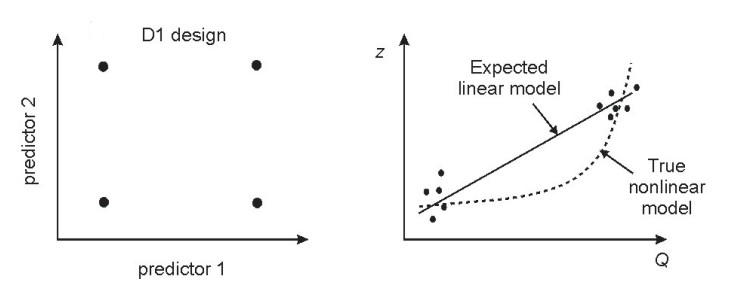
\includegraphics[width=0.9\linewidth]{./img/Fig_D1_design_scheme} 

}

\caption{Example of D1 design: (left) D1 design in 2D feature space, (right) D1 design is optimal only for linear model, if the model is curvilinear, it is in fact the worse design than simple random sampling.}\label{fig:scheme-d1}
\end{figure}

In practice we may not know what is the nature of the relationship
between \(Y\) and \(X\), i.e.~we do not wish to take a risk and produce
biased estimation. Hence we can assume that it could be a curvilinear
relationship and so we need to sample uniformly in the feature space.

\hypertarget{spatial-sampling-algorithms-of-interest}{%
\section{Spatial sampling algorithms of interest}\label{spatial-sampling-algorithms-of-interest}}

This chapter reviews some common approaches for preparing point samples for a
study area that you are visiting for the first time and/or no previous samples or
models are available. We focus on the following spatial sampling methods:

\begin{itemize}
\tightlist
\item
  Subjective or convenience sampling,
\item
  Simple Random Sampling (\textbf{SRS}) \citep{Bivand2013Springer, Brus2021sampling},
\item
  Latin Hypercube Sampling (\textbf{LHS}) and its variants e.g.~Conditioned LHS \citep{minasny2006conditioned, Malone2019PeerJ},
\item
  Feature Space Coverage Sampling (\textbf{FSCS}) \citep{Goerg2013} and fuzzy k-means clustering \citep{hastie2009elements},
\item
  2nd round sampling \citep{stumpf2017uncertainty},
\end{itemize}

Our interest in this tutorials is in producing predictions (maps) of the target
variable by employing regression / correlation between the target variable and
multitude of features (raster layers), and where various Machine Learning techniques
are used for training and prediction.

Once we collect enough training points in an area we can overlay points and GIS
layers to produce a \textbf{regression matrix} or \textbf{classification matrix}, and
which can then be used to generate spatial predictions i.e.~produce maps. As a
state-of-the-art we use the mlr framework for Ensemble Machine Learning as the key
Machine Learning framework for predictive mapping. For an introduction to Ensemble
Machine Learning for Predictive Mapping please refer to \href{https://gitlab.com/openlandmap/spatial-predictions-using-eml}{this tutorial}.

\hypertarget{ebergotzen-dataset}{%
\section{Ebergotzen dataset}\label{ebergotzen-dataset}}

To test various sampling and mapping algorithms, we can use the Ebergotzen
dataset available also via the \textbf{plotKML} package \citep{hengl2015plotkml}:

\begin{Shaded}
\begin{Highlighting}[]
\FunctionTok{set.seed}\NormalTok{(}\DecValTok{100}\NormalTok{)}
\FunctionTok{library}\NormalTok{(plotKML)}
\FunctionTok{library}\NormalTok{(sp)}
\FunctionTok{library}\NormalTok{(viridis)}
\CommentTok{\#\textgreater{} Loading required package: viridisLite}
\FunctionTok{library}\NormalTok{(raster)}
\FunctionTok{library}\NormalTok{(ggplot2)}
\FunctionTok{data}\NormalTok{(}\StringTok{"eberg\_grid25"}\NormalTok{)}
\FunctionTok{gridded}\NormalTok{(eberg\_grid25) }\OtherTok{\textless{}{-}} \ErrorTok{\textasciitilde{}}\NormalTok{x}\SpecialCharTok{+}\NormalTok{y}
\FunctionTok{proj4string}\NormalTok{(eberg\_grid25) }\OtherTok{\textless{}{-}} \FunctionTok{CRS}\NormalTok{(}\StringTok{"+init=epsg:31467"}\NormalTok{)}
\end{Highlighting}
\end{Shaded}

This dataset is described in detail in \citet{Bohner2008Hamburg}. It is a soil survey
dataset with ground observations and measurements of soil properties including soil
types. The study area is a perfect square 10×10 km in size.

We have previously derived number of additional DEM parameters directly using SAGA GIS
\citep{Conrad2015} and which we can add to the list of covariates:

\begin{Shaded}
\begin{Highlighting}[]
\NormalTok{eberg\_grid25 }\OtherTok{=} \FunctionTok{cbind}\NormalTok{(eberg\_grid25, }\FunctionTok{readRDS}\NormalTok{(}\StringTok{"./extdata/eberg\_dtm\_25m.rds"}\NormalTok{))}
\FunctionTok{names}\NormalTok{(eberg\_grid25)}
\CommentTok{\#\textgreater{}  [1] "DEMTOPx"        "HBTSOLx"        "TWITOPx"        "NVILANx"       }
\CommentTok{\#\textgreater{}  [5] "eberg\_dscurv"   "eberg\_hshade"   "eberg\_lsfactor" "eberg\_pcurv"   }
\CommentTok{\#\textgreater{}  [9] "eberg\_slope"    "eberg\_stwi"     "eberg\_twi"      "eberg\_vdepth"  }
\CommentTok{\#\textgreater{} [13] "PMTZONES"}
\end{Highlighting}
\end{Shaded}

so a total of 11 layers at 25-m spatial resolution, from which two layers
(\texttt{HBTSOLx} and \texttt{PMTZONES}) are factors representing soil units and parent material
units. Next, for further analysis, and to reduce data overlap, we can convert all
primary variables to (numeric) principal components using:

\begin{Shaded}
\begin{Highlighting}[]
\NormalTok{eberg\_spc }\OtherTok{=}\NormalTok{ landmap}\SpecialCharTok{::}\FunctionTok{spc}\NormalTok{(eberg\_grid25[}\SpecialCharTok{{-}}\FunctionTok{c}\NormalTok{(}\DecValTok{2}\NormalTok{,}\DecValTok{3}\NormalTok{)])}
\CommentTok{\#\textgreater{} Converting PMTZONES to indicators...}
\CommentTok{\#\textgreater{} Converting covariates to principal components...}
\end{Highlighting}
\end{Shaded}

which gives the a total of 14 PCs. The patterns in the PC components reflect
a complex combination of terrain variables, lithological discontinuities (\texttt{PMTZONES})
and surface vegetation (\texttt{NVILANx}):

\begin{Shaded}
\begin{Highlighting}[]
\FunctionTok{spplot}\NormalTok{(eberg\_spc}\SpecialCharTok{@}\NormalTok{predicted[}\DecValTok{1}\SpecialCharTok{:}\DecValTok{3}\NormalTok{], }\AttributeTok{col.regions=}\NormalTok{SAGA\_pal[[}\DecValTok{1}\NormalTok{]])}
\end{Highlighting}
\end{Shaded}

\begin{figure}

{\centering \includegraphics[width=1\linewidth]{./img/Fig_PCA_components_Ebergotzen} 

}

\caption{Principal Components derived using Ebergotzen dataset.}\label{fig:plot-spc}
\end{figure}

\hypertarget{simple-random-sampling}{%
\section{Simple Random Sampling}\label{simple-random-sampling}}

To generate a SRS with e.g.~100 points we can use the \textbf{sp} package \texttt{spsample} method:

\begin{Shaded}
\begin{Highlighting}[]
\NormalTok{rnd }\OtherTok{\textless{}{-}} \FunctionTok{spsample}\NormalTok{(eberg\_grid25[}\DecValTok{1}\NormalTok{], }\AttributeTok{type=}\StringTok{"random"}\NormalTok{, }\AttributeTok{n=}\DecValTok{100}\NormalTok{)}
\end{Highlighting}
\end{Shaded}

\begin{Shaded}
\begin{Highlighting}[]
\FunctionTok{plot}\NormalTok{(}\FunctionTok{raster}\NormalTok{(eberg\_spc}\SpecialCharTok{@}\NormalTok{predicted[}\DecValTok{1}\NormalTok{]), }\AttributeTok{col=}\NormalTok{SAGA\_pal[[}\DecValTok{1}\NormalTok{]])}
\FunctionTok{points}\NormalTok{(rnd, }\AttributeTok{pch=}\StringTok{"+"}\NormalTok{)}
\end{Highlighting}
\end{Shaded}

\begin{figure}

{\centering 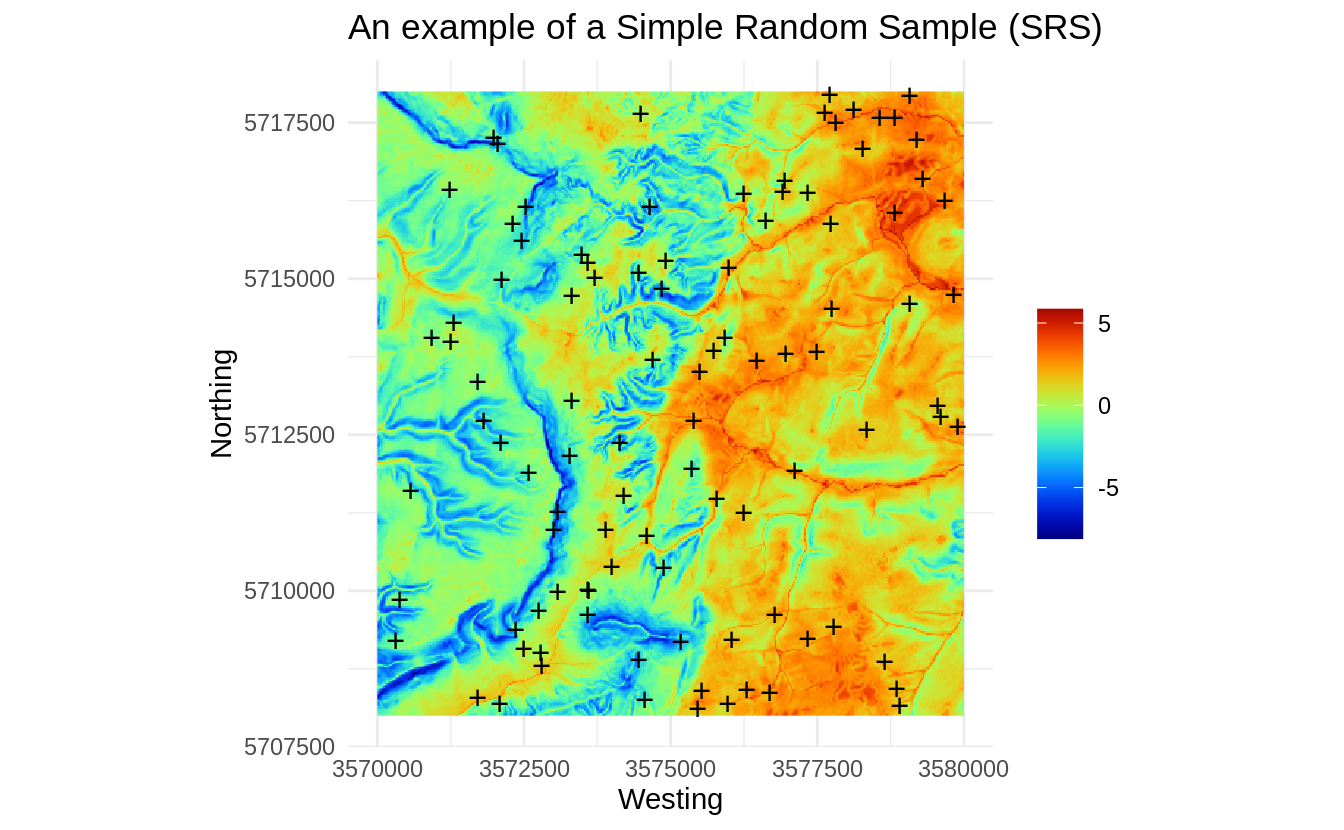
\includegraphics[width=0.8\linewidth]{sampling_files/figure-latex/eberg-srs-1} 

}

\caption{An example of a Simple Random Sample (SRS).}\label{fig:eberg-srs}
\end{figure}

This sample is generated purely based on the spatial domain, the feature space
is completely ignored / not taken into account, hence we can check how well do
these points represent the feature space using a density plot:

\begin{Shaded}
\begin{Highlighting}[]
\NormalTok{ov.rnd }\OtherTok{=}\NormalTok{ sp}\SpecialCharTok{::}\FunctionTok{over}\NormalTok{(rnd, eberg\_spc}\SpecialCharTok{@}\NormalTok{predicted[,}\DecValTok{1}\SpecialCharTok{:}\DecValTok{2}\NormalTok{])}
\FunctionTok{library}\NormalTok{(hexbin)}
\FunctionTok{library}\NormalTok{(grid)}
\NormalTok{reds }\OtherTok{=} \FunctionTok{colorRampPalette}\NormalTok{(RColorBrewer}\SpecialCharTok{::}\FunctionTok{brewer.pal}\NormalTok{(}\DecValTok{9}\NormalTok{, }\StringTok{"YlOrRd"}\NormalTok{)[}\SpecialCharTok{{-}}\DecValTok{1}\NormalTok{])}
\NormalTok{hb }\OtherTok{\textless{}{-}} \FunctionTok{hexbin}\NormalTok{(eberg\_spc}\SpecialCharTok{@}\NormalTok{predicted}\SpecialCharTok{@}\NormalTok{data[,}\DecValTok{1}\SpecialCharTok{:}\DecValTok{2}\NormalTok{], }\AttributeTok{xbins=}\DecValTok{60}\NormalTok{)}
\NormalTok{p }\OtherTok{\textless{}{-}} \FunctionTok{plot}\NormalTok{(hb, }\AttributeTok{colramp =}\NormalTok{ reds, }\AttributeTok{main=}\StringTok{\textquotesingle{}PCA Ebergotzen SRS\textquotesingle{}}\NormalTok{)}
\FunctionTok{pushHexport}\NormalTok{(p}\SpecialCharTok{$}\NormalTok{plot.vp)}
\FunctionTok{grid.points}\NormalTok{(ov.rnd[,}\DecValTok{1}\NormalTok{], ov.rnd[,}\DecValTok{2}\NormalTok{], }\AttributeTok{pch=}\StringTok{"+"}\NormalTok{)}
\end{Highlighting}
\end{Shaded}

\begin{figure}

{\centering 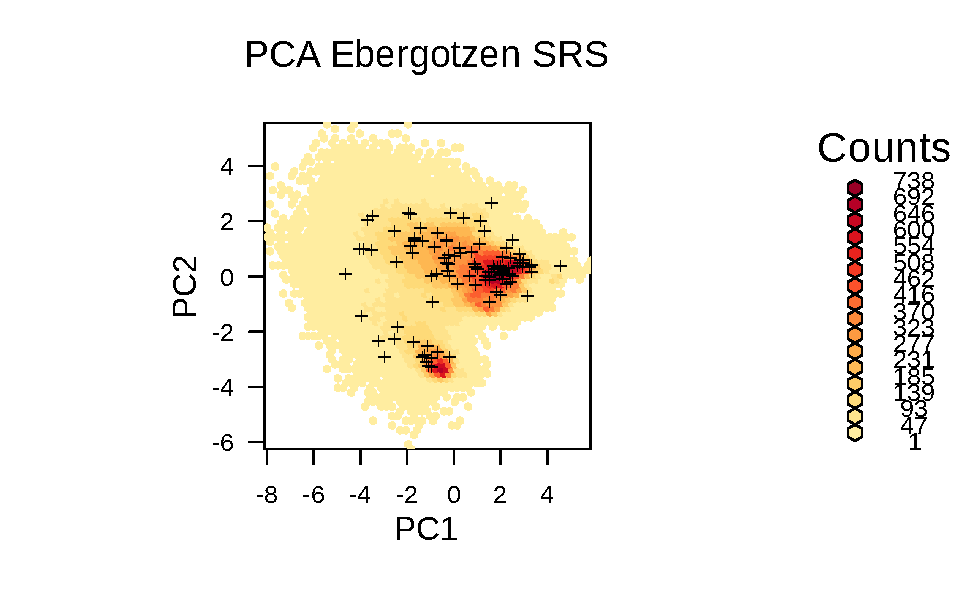
\includegraphics[width=0.8\linewidth]{sampling_files/figure-latex/eberg-fs-1} 

}

\caption{Distribution of the SRS points from the previous example in the feature space.}\label{fig:eberg-fs}
\end{figure}

Visually, we do not directly see from Fig. \ref{fig:eberg-fs} that the generated SRS
maybe misses some important feature space, however if we zoom in, then we can notice that some
parts of feature space (in this specific randomization) with high density are somewhat
under-represented. Imagine if we reduce number of sampling points then we run
even higher risk of missing some areas in the feature space by using SRS.

Next, we are interested in evaluating the occurrence probability of the SRS points
based on the PCA components. To derive the occurrence probability we can use
the \textbf{maxlike} package method \citep{Royle2012}:

\begin{Shaded}
\begin{Highlighting}[]
\NormalTok{fm.cov }\OtherTok{\textless{}{-}}\NormalTok{ stats}\SpecialCharTok{::}\FunctionTok{as.formula}\NormalTok{(}\FunctionTok{paste}\NormalTok{(}\StringTok{"\textasciitilde{}"}\NormalTok{, }\FunctionTok{paste}\NormalTok{(}\FunctionTok{names}\NormalTok{(eberg\_spc}\SpecialCharTok{@}\NormalTok{predicted[}\DecValTok{1}\SpecialCharTok{:}\DecValTok{4}\NormalTok{]), }\AttributeTok{collapse=}\StringTok{"+"}\NormalTok{)))}
\NormalTok{ml }\OtherTok{\textless{}{-}}\NormalTok{ maxlike}\SpecialCharTok{::}\FunctionTok{maxlike}\NormalTok{(}\AttributeTok{formula=}\NormalTok{fm.cov, }\AttributeTok{rasters=}\NormalTok{raster}\SpecialCharTok{::}\FunctionTok{stack}\NormalTok{(eberg\_spc}\SpecialCharTok{@}\NormalTok{predicted[}\DecValTok{1}\SpecialCharTok{:}\DecValTok{4}\NormalTok{]), }
                       \AttributeTok{points=}\NormalTok{rnd}\SpecialCharTok{@}\NormalTok{coords, }\AttributeTok{method=}\StringTok{"BFGS"}\NormalTok{, }\AttributeTok{removeDuplicates=}\ConstantTok{TRUE}\NormalTok{, }\AttributeTok{savedata=}\ConstantTok{TRUE}\NormalTok{)}
\NormalTok{ml.prob }\OtherTok{\textless{}{-}} \FunctionTok{predict}\NormalTok{(ml)}
\end{Highlighting}
\end{Shaded}

\begin{Shaded}
\begin{Highlighting}[]
\FunctionTok{plot}\NormalTok{(ml.prob)}
\FunctionTok{points}\NormalTok{(rnd}\SpecialCharTok{@}\NormalTok{coords, }\AttributeTok{pch=}\StringTok{"+"}\NormalTok{)}
\end{Highlighting}
\end{Shaded}

\begin{figure}

{\centering 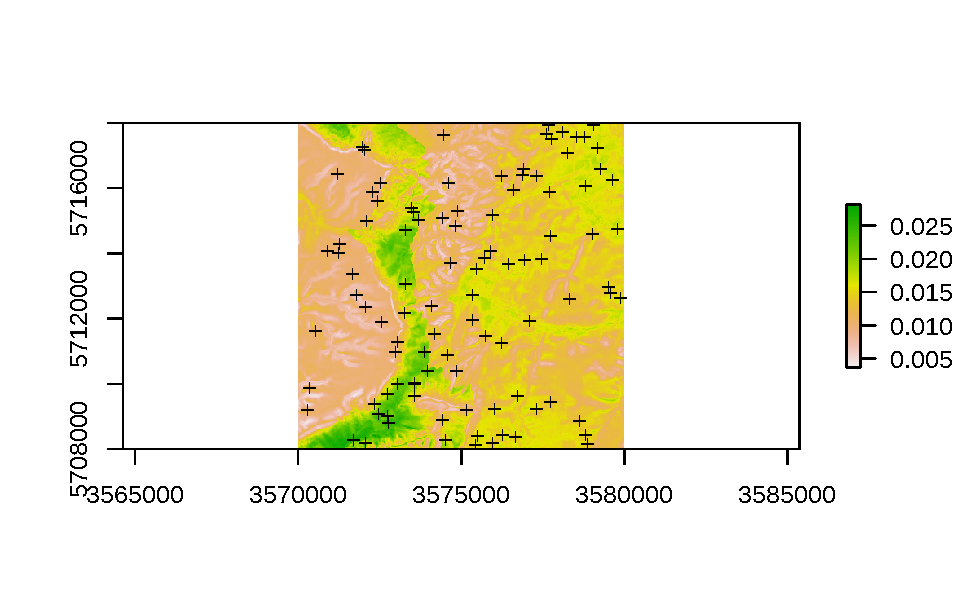
\includegraphics[width=0.8\linewidth]{sampling_files/figure-latex/eberg-maxlike-1} 

}

\caption{Occurrence probability for SRS derived using the maxlike package.}\label{fig:eberg-maxlike}
\end{figure}

Note: for the sake of reducing the computing intensity we focus on the first four PCs.
In practice, feature space analysis can be quite computational and we recommend using
parallelized versions within an High Performance Computing environments to run such analysis.

Fig. \ref{fig:eberg-maxlike} shows that, by accident, some parts of the feature
space might be somewhat under-represented (areas with low probability of occurrence on the map).
Note however that occurrence probability for this dataset is overall \emph{very low} (\textless0.05),
indicating that distribution of points is not much correlated with the features.
This specific SRS is thus probably satisfactory also for feature space analysis:
the SRS points do not seem to group (which would in this case be by accident) and
hence maxlike gives very low probability of occurrence.

We can repeat SRS many times and then see if the clustering of points gets more
problematic, but as you can image, in practice for large number of samples it is
a good chance that all features would get well represented also in the feature
space even though we did not include feature space variables in the production of the
sampling plan.

We can now also load the actual points collected for the Ebergotzen case study:

\begin{Shaded}
\begin{Highlighting}[]
\FunctionTok{data}\NormalTok{(eberg)}
\NormalTok{eberg.xy }\OtherTok{\textless{}{-}}\NormalTok{ eberg[,}\FunctionTok{c}\NormalTok{(}\StringTok{"X"}\NormalTok{,}\StringTok{"Y"}\NormalTok{)]}
\FunctionTok{coordinates}\NormalTok{(eberg.xy) }\OtherTok{\textless{}{-}} \ErrorTok{\textasciitilde{}}\NormalTok{X}\SpecialCharTok{+}\NormalTok{Y}
\FunctionTok{proj4string}\NormalTok{(eberg.xy) }\OtherTok{\textless{}{-}} \FunctionTok{CRS}\NormalTok{(}\StringTok{"+init=epsg:31467"}\NormalTok{)}
\NormalTok{ov.xy }\OtherTok{=}\NormalTok{ sp}\SpecialCharTok{::}\FunctionTok{over}\NormalTok{(eberg.xy, eberg\_grid25[}\DecValTok{1}\NormalTok{])}
\NormalTok{eberg.xy }\OtherTok{=}\NormalTok{ eberg.xy[}\SpecialCharTok{!}\FunctionTok{is.na}\NormalTok{(ov.xy}\SpecialCharTok{$}\NormalTok{DEMTOPx),]}
\NormalTok{sel }\OtherTok{\textless{}{-}} \FunctionTok{sample.int}\NormalTok{(}\FunctionTok{length}\NormalTok{(eberg.xy), }\DecValTok{100}\NormalTok{)}
\NormalTok{eberg.smp }\OtherTok{=}\NormalTok{ eberg.xy[sel,]}
\end{Highlighting}
\end{Shaded}

To quickly estimate spread of points in geographical and feature spaces, we can
also use the function \texttt{spsample.prob} that calls both the kernel density function
from the \textbf{\href{https://rdrr.io/cran/spatstat.core/man/density.ppp.html}{spatstat}} package, and derives the probability of occurrence using the
\textbf{\href{https://rdrr.io/github/rbchan/maxlike/man/maxlike-package.html}{maxlike}} package:

\begin{Shaded}
\begin{Highlighting}[]
\NormalTok{iprob }\OtherTok{\textless{}{-}}\NormalTok{ landmap}\SpecialCharTok{::}\FunctionTok{spsample.prob}\NormalTok{(eberg.smp, eberg\_spc}\SpecialCharTok{@}\NormalTok{predicted[}\DecValTok{1}\SpecialCharTok{:}\DecValTok{4}\NormalTok{])}
\CommentTok{\#\textgreater{} Deriving kernel density map using sigma 1010 ...}
\CommentTok{\#\textgreater{} Deriving inclusion probabilities using MaxLike analysis...}
\end{Highlighting}
\end{Shaded}

In this specific case, the actual sampling points are much more clustered, so if we plot
the two occurrence probability maps derived using maxlike next to each other (actual vs SRS) we get:

\begin{Shaded}
\begin{Highlighting}[]
\NormalTok{op }\OtherTok{\textless{}{-}} \FunctionTok{par}\NormalTok{(}\AttributeTok{mfrow=}\FunctionTok{c}\NormalTok{(}\DecValTok{1}\NormalTok{,}\DecValTok{2}\NormalTok{))}
\FunctionTok{plot}\NormalTok{(}\FunctionTok{raster}\NormalTok{(iprob}\SpecialCharTok{$}\NormalTok{maxlike), }\AttributeTok{zlim=}\FunctionTok{c}\NormalTok{(}\DecValTok{0}\NormalTok{,}\DecValTok{1}\NormalTok{))}
\FunctionTok{points}\NormalTok{(eberg.smp}\SpecialCharTok{@}\NormalTok{coords, }\AttributeTok{pch=}\StringTok{"+"}\NormalTok{)}
\FunctionTok{plot}\NormalTok{(ml.prob, }\AttributeTok{zlim=}\FunctionTok{c}\NormalTok{(}\DecValTok{0}\NormalTok{,}\DecValTok{1}\NormalTok{))}
\FunctionTok{points}\NormalTok{(rnd}\SpecialCharTok{@}\NormalTok{coords, }\AttributeTok{pch=}\StringTok{"+"}\NormalTok{)}
\FunctionTok{par}\NormalTok{(op)}
\end{Highlighting}
\end{Shaded}

\begin{figure}

{\centering 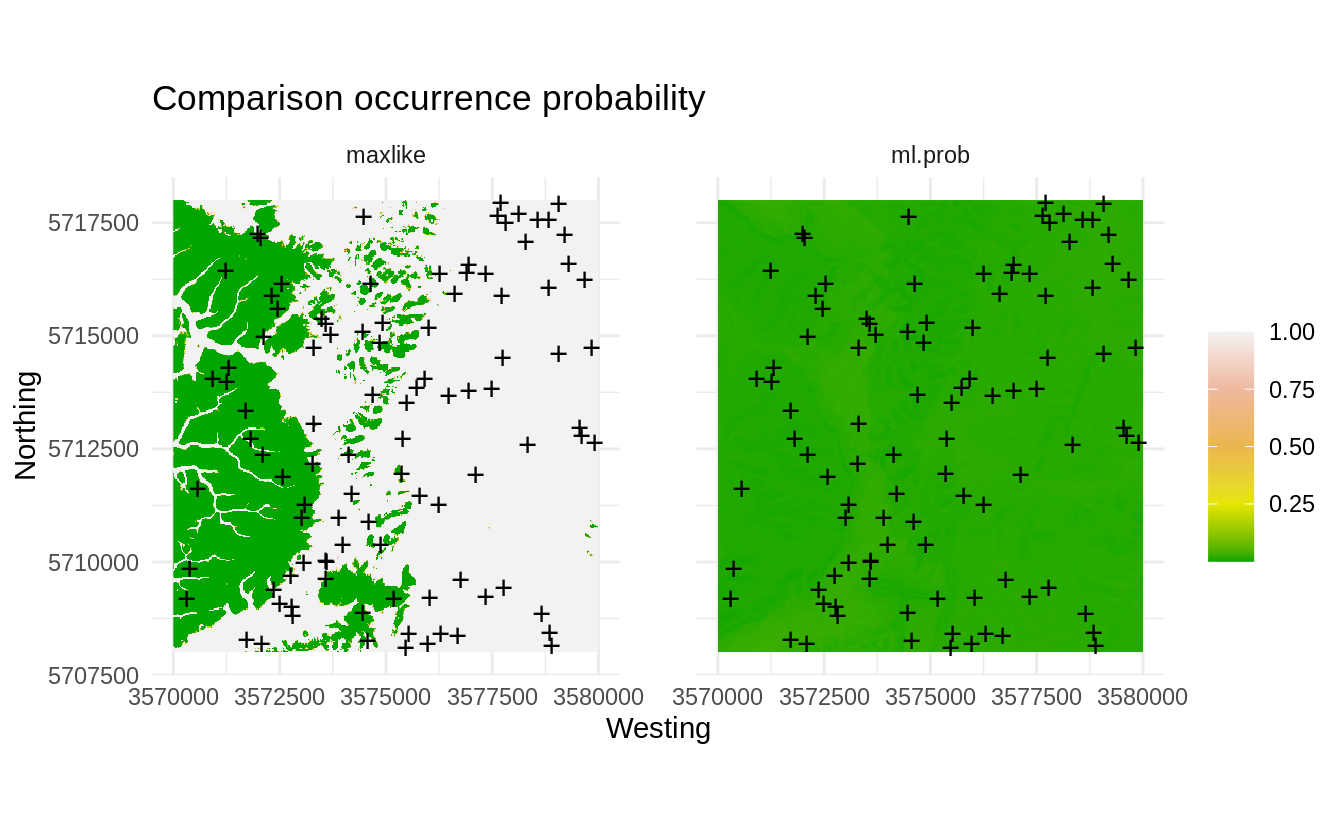
\includegraphics[width=1\linewidth]{sampling_files/figure-latex/eberg-maxlike2-1} 

}

\caption{Comparison occurrence probability for actual and SRS samples derived using the maxlike package.}\label{fig:eberg-maxlike2}
\end{figure}

The map on the left clearly indicates that most of the sampling points are
basically preferentially located in the plain area, while the hillands are
systematically under-sampled. This we can also cross-check by reading the
description of the dataset in \citet{Bohner2008Hamburg}:

\begin{itemize}
\tightlist
\item
  the Ebergotzen soil survey points focus on agricultural land only,\\
\item
  no objective sampling design has been used, hence some points are clustered,
\end{itemize}

This is also clearly visible from the \emph{feature map} plot where one part of the feature
space seem to be completely omitted from sampling:

\begin{Shaded}
\begin{Highlighting}[]
\NormalTok{ov2.rnd }\OtherTok{=}\NormalTok{ sp}\SpecialCharTok{::}\FunctionTok{over}\NormalTok{(eberg.smp, eberg\_spc}\SpecialCharTok{@}\NormalTok{predicted[,}\DecValTok{1}\SpecialCharTok{:}\DecValTok{2}\NormalTok{])}
\NormalTok{p }\OtherTok{\textless{}{-}} \FunctionTok{plot}\NormalTok{(hb, }\AttributeTok{colramp =}\NormalTok{ reds, }\AttributeTok{main=}\StringTok{\textquotesingle{}PCA Ebergotzen actual\textquotesingle{}}\NormalTok{)}
\FunctionTok{pushHexport}\NormalTok{(p}\SpecialCharTok{$}\NormalTok{plot.vp)}
\FunctionTok{grid.points}\NormalTok{(ov2.rnd[,}\DecValTok{1}\NormalTok{], ov2.rnd[,}\DecValTok{2}\NormalTok{], }\AttributeTok{pch=}\StringTok{"+"}\NormalTok{)}
\end{Highlighting}
\end{Shaded}

\begin{figure}

{\centering 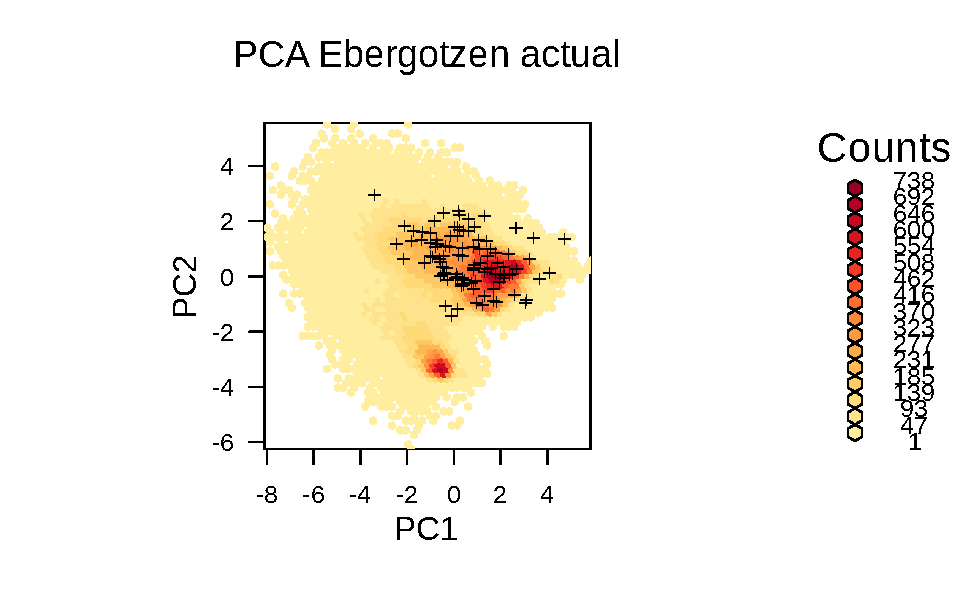
\includegraphics[width=0.8\linewidth]{sampling_files/figure-latex/eberg-fs2-1} 

}

\caption{Distribution of the actual survey points from the previous example displayed in the feature space.}\label{fig:eberg-fs2}
\end{figure}

\hypertarget{latin-hypercube-sampling}{%
\section{Latin Hypercube Sampling}\label{latin-hypercube-sampling}}

In the previous example we have shown how to implement SRS and then also evaluate it
against feature layers. Often SRS represent very well feature space so it can be
directly used for Machine Learning and with a guarantee of not making too much bias\\
in predictions. To avoid, however, risk of missing out some parts of the feature space,
and also to try to optimize allocation of points, we can generate a sample using the
\textbf{\href{https://en.wikipedia.org/wiki/Latin_hypercube_sampling}{Latin Hypercube Sampling}} (LHS) method. In a nutshell, LHS methods are based on
dividing the \textbf{Cumulative Density Function} (CDF) into \emph{n} equal partitions, and
then choosing a random data point in each partition, consequently:

\begin{itemize}
\tightlist
\item
  CDF of LHS samples matches the CDF of population (hence unbiased representation),\\
\item
  Extrapolation in the feature space should be minimized,
\end{itemize}

Latin Hypercube and sampling optimization using LHS is explained in detail in \citet{minasny2006conditioned}
and \citet{shields2016generalization}. For \citet{brus2015balanced}, LHS is just a special case
of \textbf{\href{http://www.antongrafstrom.se/balancedsampling/}{balanced sampling}} i.e.~sampling based on allocation in feature space.
The \href{https://github.com/bertcarnell/lhs}{lhs package} also contains numerous examples of
how to implement LHS for (non-spatial) data.

Here we use an implementation of the LHS available in the \textbf{clhs} package \citep{Roudier2011}:

\begin{Shaded}
\begin{Highlighting}[]
\FunctionTok{library}\NormalTok{(clhs)}
\NormalTok{rnd.lhs }\OtherTok{=}\NormalTok{ clhs}\SpecialCharTok{::}\FunctionTok{clhs}\NormalTok{(eberg\_spc}\SpecialCharTok{@}\NormalTok{predicted[}\DecValTok{1}\SpecialCharTok{:}\DecValTok{4}\NormalTok{], }\AttributeTok{size=}\DecValTok{100}\NormalTok{, }\AttributeTok{iter=}\DecValTok{100}\NormalTok{, }\AttributeTok{progress=}\ConstantTok{FALSE}\NormalTok{)}
\end{Highlighting}
\end{Shaded}

This actually implements the so-called \emph{``Conditional LHS''} \citep{minasny2006conditioned},
and can get quite computational for large stack of rasters, hence we manually limit the
number of iterations to 100.

We can plot the LHS sampling plan:

\begin{Shaded}
\begin{Highlighting}[]
\FunctionTok{plot}\NormalTok{(}\FunctionTok{raster}\NormalTok{(eberg\_spc}\SpecialCharTok{@}\NormalTok{predicted[}\DecValTok{1}\NormalTok{]), }\AttributeTok{col=}\NormalTok{SAGA\_pal[[}\DecValTok{1}\NormalTok{]])}
\FunctionTok{points}\NormalTok{(rnd.lhs}\SpecialCharTok{@}\NormalTok{coords, }\AttributeTok{pch=}\StringTok{"+"}\NormalTok{)}
\end{Highlighting}
\end{Shaded}

\begin{figure}

{\centering 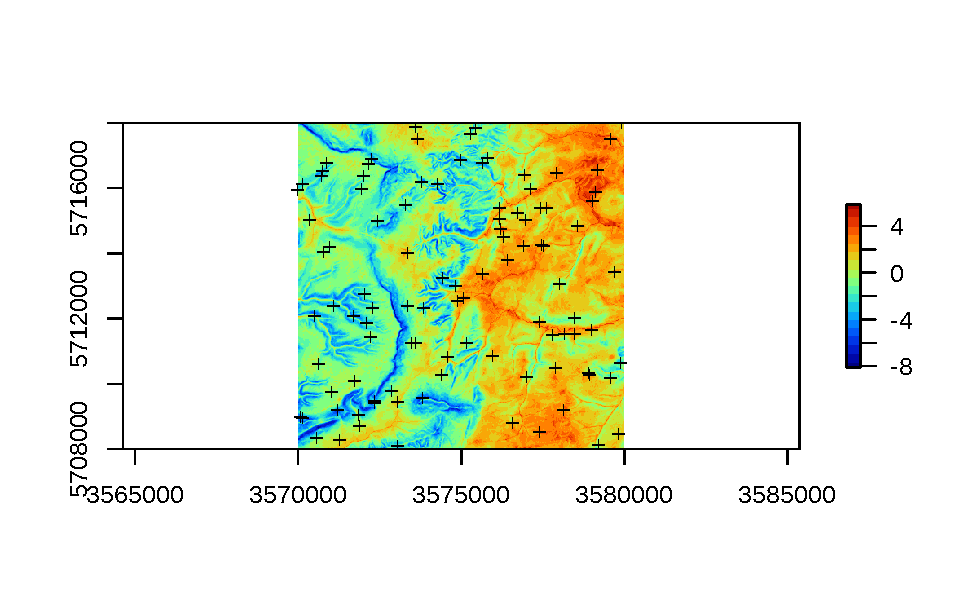
\includegraphics[width=0.8\linewidth]{sampling_files/figure-latex/eberg-clhs-1} 

}

\caption{An example of a Latin Hypercube Sample (LHS).}\label{fig:eberg-clhs}
\end{figure}

\begin{Shaded}
\begin{Highlighting}[]
\NormalTok{p }\OtherTok{\textless{}{-}} \FunctionTok{plot}\NormalTok{(hb, }\AttributeTok{colramp =}\NormalTok{ reds, }\AttributeTok{main=}\StringTok{\textquotesingle{}PCA Ebergotzen LHS\textquotesingle{}}\NormalTok{)}
\FunctionTok{pushHexport}\NormalTok{(p}\SpecialCharTok{$}\NormalTok{plot.vp)}
\FunctionTok{grid.points}\NormalTok{(rnd.lhs}\SpecialCharTok{$}\NormalTok{PC1, rnd.lhs}\SpecialCharTok{$}\NormalTok{PC2, }\AttributeTok{pch=}\StringTok{"+"}\NormalTok{)}
\end{Highlighting}
\end{Shaded}

\begin{figure}

{\centering 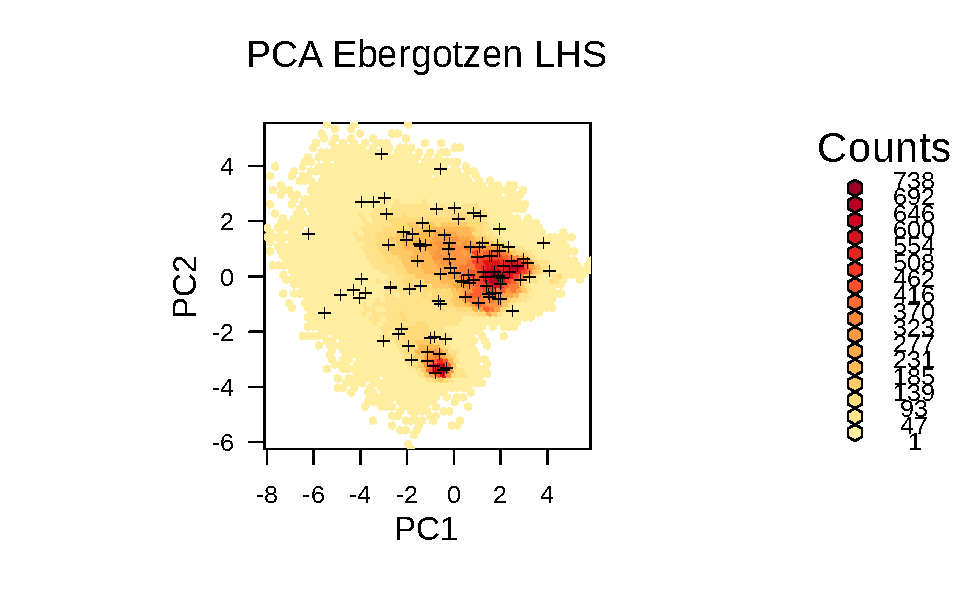
\includegraphics[width=0.8\linewidth]{sampling_files/figure-latex/eberg-lhs2-1} 

}

\caption{Distribution of the LHS points from the previous example displayed in the feature space.}\label{fig:eberg-lhs2}
\end{figure}

Although in principle we might not see any difference in the point pattern between
SRS and LHS, the feature space plot clearly shows that LHS covers systematically
feature space map, i.e.~we would have a relatively low risk of missing out some
important features as compared to Fig. \ref{fig:eberg-fs2}.

Thus the main advantages of the LHS are:

\begin{itemize}
\tightlist
\item
  it ensures that feature space is represented systematically i.e.~it is optimized
  for Machine Learning using the specific feature layers;\\
\item
  it is an \textbf{\href{https://xzhu0027.gitbook.io/blog/ml-system/sys-ml-index/learning-from-non-iid-data}{Independent Identically Distributed (IID)}} sampling design;\\
\item
  thanks to the \textbf{clhs} package, also the survey costs raster layer can be integrated to still
  keep systematic spread, but reduce survey costs as much as possible \citep{roudier2012conditioned};
\end{itemize}

\hypertarget{feature-space-coverage-sampling}{%
\section{Feature Space Coverage Sampling}\label{feature-space-coverage-sampling}}

The \textbf{Feature Space Coverage Sampling} (FSCS) is described in detail in \citet{BRUS2019464}.
In a nutshell, FSCS aims at optimal coverage of the feature space which is achieved
by minimizing the average distance of the population units (raster cells) to the
nearest sampling units in the feature space represented by the raster layers \citep{ma2020comparison}.

To produce FSCS point sample we can use function \texttt{kmeanspp} of package \textbf{LICORS} \citep{Goerg2013}.
First we partition the feature space cube to e.g.~100 clusters. We then select raster cells
with the shortest scaled Euclidean distance in covariate-space to the centers of
the clusters as the sampling units:

\begin{Shaded}
\begin{Highlighting}[]
\FunctionTok{library}\NormalTok{(LICORS)}
\FunctionTok{library}\NormalTok{(fields)}
\NormalTok{fscs.clust }\OtherTok{\textless{}{-}} \FunctionTok{kmeanspp}\NormalTok{(eberg\_spc}\SpecialCharTok{@}\NormalTok{predicted}\SpecialCharTok{@}\NormalTok{data[,}\DecValTok{1}\SpecialCharTok{:}\DecValTok{4}\NormalTok{], }\AttributeTok{k=}\DecValTok{100}\NormalTok{, }\AttributeTok{iter.max=}\DecValTok{100}\NormalTok{)}
\NormalTok{D }\OtherTok{\textless{}{-}}\NormalTok{ fields}\SpecialCharTok{::}\FunctionTok{rdist}\NormalTok{(}\AttributeTok{x1 =}\NormalTok{ fscs.clust}\SpecialCharTok{$}\NormalTok{centers, }\AttributeTok{x2 =}\NormalTok{ eberg\_spc}\SpecialCharTok{@}\NormalTok{predicted}\SpecialCharTok{@}\NormalTok{data[,}\DecValTok{1}\SpecialCharTok{:}\DecValTok{4}\NormalTok{])}
\NormalTok{units }\OtherTok{\textless{}{-}} \FunctionTok{apply}\NormalTok{(D, }\AttributeTok{MARGIN =} \DecValTok{1}\NormalTok{, }\AttributeTok{FUN =}\NormalTok{ which.min)}
\NormalTok{rnd.fscs }\OtherTok{\textless{}{-}}\NormalTok{ eberg\_spc}\SpecialCharTok{@}\NormalTok{predicted}\SpecialCharTok{@}\NormalTok{coords[units,]}
\end{Highlighting}
\end{Shaded}

Note: the k-means++ algorithm is of most interest for small sample sizes: \emph{``for large
sample sizes the extra time needed for computing the initial centers can become
substantial and may not outweigh the larger number of starts that can be afforded
with the usual k-means algorithm for the same computing time''} \citep{Brus2021sampling}.
The \texttt{kmeanspp} algorithm from the LICORS package is unfortunately quite computational
and is in principle not recommended for large grids / to generate large number of
samples. Instead, we recommend clustering feature space using the \texttt{h2o.kmeans} function
from the \href{https://docs.h2o.ai/h2o/latest-stable/h2o-docs/data-science/k-means.html}{h2o
package},
which is also suitable for larger datasets with computing running in parallel:

\begin{Shaded}
\begin{Highlighting}[]
\FunctionTok{library}\NormalTok{(h2o)}
\FunctionTok{h2o.init}\NormalTok{(}\AttributeTok{nthreads =} \SpecialCharTok{{-}}\DecValTok{1}\NormalTok{)}
\CommentTok{\#\textgreater{} }
\CommentTok{\#\textgreater{} H2O is not running yet, starting it now...}
\CommentTok{\#\textgreater{} }
\CommentTok{\#\textgreater{} Note:  In case of errors look at the following log files:}
\CommentTok{\#\textgreater{}     /tmp/Rtmp5cIwxE/file384154879baa/h2o\_tomislav\_started\_from\_r.out}
\CommentTok{\#\textgreater{}     /tmp/Rtmp5cIwxE/file38414acf64e1/h2o\_tomislav\_started\_from\_r.err}
\CommentTok{\#\textgreater{} }
\CommentTok{\#\textgreater{} }
\CommentTok{\#\textgreater{} Starting H2O JVM and connecting: .. Connection successful!}
\CommentTok{\#\textgreater{} }
\CommentTok{\#\textgreater{} R is connected to the H2O cluster: }
\CommentTok{\#\textgreater{}     H2O cluster uptime:         2 seconds 76 milliseconds }
\CommentTok{\#\textgreater{}     H2O cluster timezone:       Europe/Amsterdam }
\CommentTok{\#\textgreater{}     H2O data parsing timezone:  UTC }
\CommentTok{\#\textgreater{}     H2O cluster version:        3.30.0.1 }
\CommentTok{\#\textgreater{}     H2O cluster version age:    1 year, 9 months and 24 days !!! }
\CommentTok{\#\textgreater{}     H2O cluster name:           H2O\_started\_from\_R\_tomislav\_vru837 }
\CommentTok{\#\textgreater{}     H2O cluster total nodes:    1 }
\CommentTok{\#\textgreater{}     H2O cluster total memory:   15.71 GB }
\CommentTok{\#\textgreater{}     H2O cluster total cores:    32 }
\CommentTok{\#\textgreater{}     H2O cluster allowed cores:  32 }
\CommentTok{\#\textgreater{}     H2O cluster healthy:        TRUE }
\CommentTok{\#\textgreater{}     H2O Connection ip:          localhost }
\CommentTok{\#\textgreater{}     H2O Connection port:        54321 }
\CommentTok{\#\textgreater{}     H2O Connection proxy:       NA }
\CommentTok{\#\textgreater{}     H2O Internal Security:      FALSE }
\CommentTok{\#\textgreater{}     H2O API Extensions:         Amazon S3, XGBoost, Algos, AutoML, Core V3, TargetEncoder, Core V4 }
\CommentTok{\#\textgreater{}     R Version:                  R version 4.0.2 (2020{-}06{-}22)}
\CommentTok{\#\textgreater{} Warning in h2o.clusterInfo(): }
\CommentTok{\#\textgreater{} Your H2O cluster version is too old (1 year, 9 months and 24 days)!}
\CommentTok{\#\textgreater{} Please download and install the latest version from http://h2o.ai/download/}
\NormalTok{df.hex }\OtherTok{\textless{}{-}} \FunctionTok{as.h2o}\NormalTok{(eberg\_spc}\SpecialCharTok{@}\NormalTok{predicted}\SpecialCharTok{@}\NormalTok{data[,}\DecValTok{1}\SpecialCharTok{:}\DecValTok{4}\NormalTok{], }\AttributeTok{destination\_frame =} \StringTok{"df"}\NormalTok{)}
\CommentTok{\#\textgreater{} }
  \SpecialCharTok{|}                                                                            
  \ErrorTok{|}                                                                      \ErrorTok{|}   \DecValTok{0}\NormalTok{\%}
  \SpecialCharTok{|}                                                                            
  \ErrorTok{|======================================================================|} \DecValTok{100}\NormalTok{\%}
\NormalTok{km.nut }\OtherTok{\textless{}{-}} \FunctionTok{h2o.kmeans}\NormalTok{(}\AttributeTok{training\_frame=}\NormalTok{df.hex, }\AttributeTok{k=}\DecValTok{100}\NormalTok{, }\AttributeTok{keep\_cross\_validation\_predictions =} \ConstantTok{TRUE}\NormalTok{)}
\CommentTok{\#\textgreater{} }
  \SpecialCharTok{|}                                                                            
  \ErrorTok{|}                                                                      \ErrorTok{|}   \DecValTok{0}\NormalTok{\%}
  \SpecialCharTok{|}                                                                            
  \ErrorTok{|=======}                                                               \ErrorTok{|}  \DecValTok{10}\NormalTok{\%}
  \SpecialCharTok{|}                                                                            
  \ErrorTok{|======================================================================|} \DecValTok{100}\NormalTok{\%}
\CommentTok{\#km.nut}
\end{Highlighting}
\end{Shaded}

Note: in the example above, we have manually set the number of clusters to 100,
but the number of clusters could be also derived using \href{https://www.r-bloggers.com/2019/01/10-tips-for-choosing-the-optimal-number-of-clusters/}{some optimization procedure}.
Next, we predict the clusters and plot the output:

\begin{Shaded}
\begin{Highlighting}[]
\NormalTok{m.km }\OtherTok{\textless{}{-}} \FunctionTok{as.data.frame}\NormalTok{(}\FunctionTok{h2o.predict}\NormalTok{(km.nut, df.hex, }\AttributeTok{na.action=}\NormalTok{na.pass))}
\CommentTok{\#\textgreater{} }
  \SpecialCharTok{|}                                                                            
  \ErrorTok{|}                                                                      \ErrorTok{|}   \DecValTok{0}\NormalTok{\%}
  \SpecialCharTok{|}                                                                            
  \ErrorTok{|======================================================================|} \DecValTok{100}\NormalTok{\%}
\end{Highlighting}
\end{Shaded}

We can save the class centers (if needed for any further analysis):

\begin{Shaded}
\begin{Highlighting}[]
\NormalTok{class\_df.c }\OtherTok{=} \FunctionTok{as.data.frame}\NormalTok{(}\FunctionTok{h2o.centers}\NormalTok{(km.nut))}
\FunctionTok{names}\NormalTok{(class\_df.c) }\OtherTok{=} \FunctionTok{names}\NormalTok{(eberg\_spc}\SpecialCharTok{@}\NormalTok{predicted}\SpecialCharTok{@}\NormalTok{data[,}\DecValTok{1}\SpecialCharTok{:}\DecValTok{4}\NormalTok{])}
\FunctionTok{str}\NormalTok{(class\_df.c)}
\CommentTok{\#\textgreater{} \textquotesingle{}data.frame\textquotesingle{}:    100 obs. of  4 variables:}
\CommentTok{\#\textgreater{}  $ PC1: num  1.16 {-}2.04 1.59 {-}3.25 {-}4.24 ...}
\CommentTok{\#\textgreater{}  $ PC2: num  0.734 2.287 2.355 {-}3.997 3.615 ...}
\CommentTok{\#\textgreater{}  $ PC3: num  {-}1.1588 5.5599 3.263 {-}3.7764 {-}0.0067 ...}
\CommentTok{\#\textgreater{}  $ PC4: num  0.269 4.501 {-}2.24 {-}2.661 3.304 ...}
\CommentTok{\#write.csv(class\_df.c, "NCluster\_100\_class\_centers.csv")}
\end{Highlighting}
\end{Shaded}

To select sampling points we use the minimum distance to class centers \citep{Brus2021sampling}:

\begin{Shaded}
\begin{Highlighting}[]
\NormalTok{D }\OtherTok{\textless{}{-}}\NormalTok{ fields}\SpecialCharTok{::}\FunctionTok{rdist}\NormalTok{(}\AttributeTok{x1 =}\NormalTok{ class\_df.c, }\AttributeTok{x2 =}\NormalTok{ eberg\_spc}\SpecialCharTok{@}\NormalTok{predicted}\SpecialCharTok{@}\NormalTok{data[,}\DecValTok{1}\SpecialCharTok{:}\DecValTok{4}\NormalTok{])}
\NormalTok{units }\OtherTok{\textless{}{-}} \FunctionTok{apply}\NormalTok{(D, }\AttributeTok{MARGIN =} \DecValTok{1}\NormalTok{, }\AttributeTok{FUN =}\NormalTok{ which.min)}
\NormalTok{rnd.fscs }\OtherTok{\textless{}{-}}\NormalTok{ eberg\_spc}\SpecialCharTok{@}\NormalTok{predicted}\SpecialCharTok{@}\NormalTok{coords[units,]}
\end{Highlighting}
\end{Shaded}

\begin{Shaded}
\begin{Highlighting}[]
\FunctionTok{plot}\NormalTok{(}\FunctionTok{raster}\NormalTok{(eberg\_spc}\SpecialCharTok{@}\NormalTok{predicted[}\DecValTok{1}\NormalTok{]), }\AttributeTok{col=}\NormalTok{SAGA\_pal[[}\DecValTok{1}\NormalTok{]])}
\FunctionTok{points}\NormalTok{(rnd.fscs, }\AttributeTok{pch=}\StringTok{"+"}\NormalTok{)}
\end{Highlighting}
\end{Shaded}

\begin{figure}

{\centering 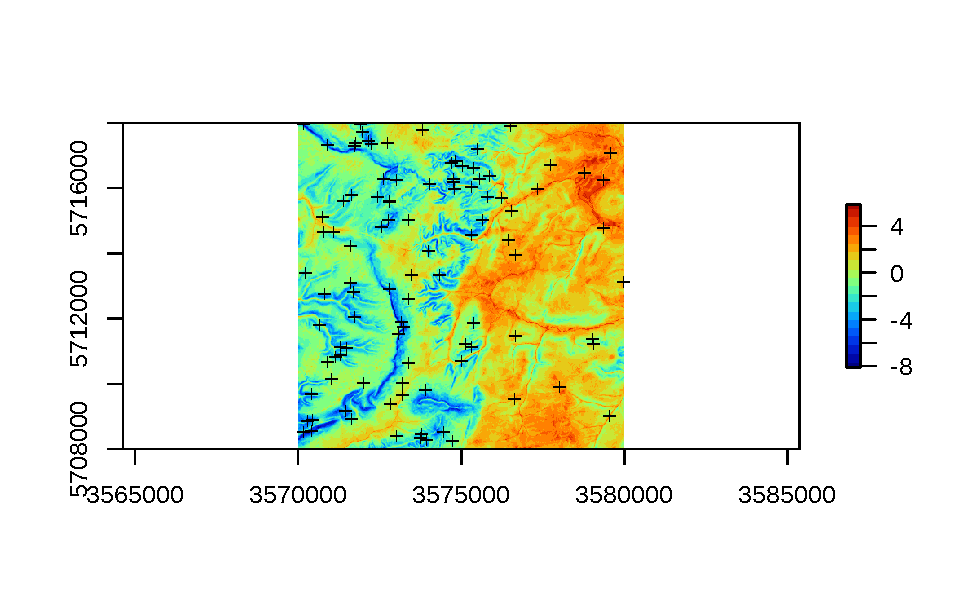
\includegraphics[width=0.8\linewidth]{sampling_files/figure-latex/eberg-fscs-1} 

}

\caption{An example of a Feature Space Coverage Sampling (FSCS).}\label{fig:eberg-fscs}
\end{figure}

Visually, FSCS seem to add higher spatial density of points in areas where there
is higher complexity. The \texttt{h2o.kmeans} algorithm stratifies area into most
possible homogeneous units (in the example above, large plains in the right
part of the study area are relatively homogeneous, hence the sampling intensity
in there areas drops significantly when visualized in the geographical space),
and the points are then allocated per each strata.

\begin{Shaded}
\begin{Highlighting}[]
\NormalTok{p }\OtherTok{\textless{}{-}} \FunctionTok{plot}\NormalTok{(hb, }\AttributeTok{colramp =}\NormalTok{ reds, }\AttributeTok{main=}\StringTok{\textquotesingle{}PCA Ebergotzen FSCS\textquotesingle{}}\NormalTok{)}
\FunctionTok{pushHexport}\NormalTok{(p}\SpecialCharTok{$}\NormalTok{plot.vp)}
\FunctionTok{grid.points}\NormalTok{(eberg\_spc}\SpecialCharTok{@}\NormalTok{predicted}\SpecialCharTok{@}\NormalTok{data[units,}\StringTok{"PC1"}\NormalTok{], eberg\_spc}\SpecialCharTok{@}\NormalTok{predicted}\SpecialCharTok{@}\NormalTok{data[units,}\StringTok{"PC2"}\NormalTok{], }\AttributeTok{pch=}\StringTok{"+"}\NormalTok{)}
\end{Highlighting}
\end{Shaded}

\begin{figure}

{\centering 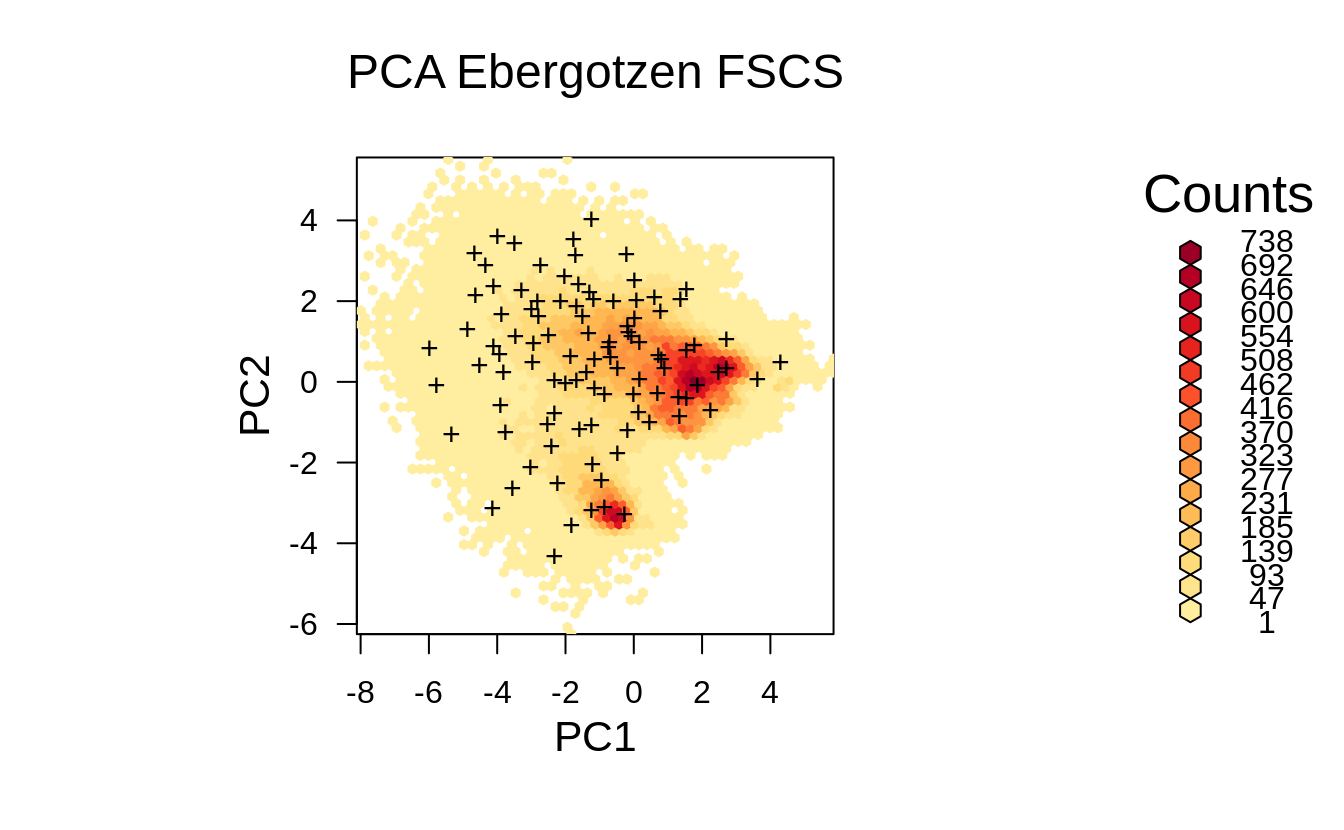
\includegraphics[width=0.8\linewidth]{sampling_files/figure-latex/eberg-fscs-pnts-1} 

}

\caption{Distribution of the FSCS points from the previous example displayed in the feature space.}\label{fig:eberg-fscs-pnts}
\end{figure}

The FSCS sampling pattern in feature space looks almost as grid sampling in feature
space. FSCS seems to put more effort on sampling at the edges on the feature space
in comparison to LHS and SRS, and hence can be compared to classical response
surface designs such as \href{https://en.wikipedia.org/wiki/Optimal_design}{D-optimal designs} \citep{Hengl2004AJSR}.

\begin{Shaded}
\begin{Highlighting}[]
\FunctionTok{h2o.shutdown}\NormalTok{(}\AttributeTok{prompt =} \ConstantTok{FALSE}\NormalTok{)}
\end{Highlighting}
\end{Shaded}

\hypertarget{summary-points}{%
\section{Summary points}\label{summary-points}}

In the previous examples we have shown differences between SRS, LHS and FSCS.
SRS and LHS are IID sampling methods and as long as the number of samples is large
and the study area is complex, it is often difficult to notice or quantify any under- or
over-sampling. Depending on which variant of FSCS we implement, FSCS can result in
higher spatial spreading especially if a study area consists of a combination
of a relatively homogeneous and complex terrain units.

The Ebergotzen dataset (existing point samples) clearly shows that the \emph{``convenience surveys''} can
show significant clustering and under-representation of feature space
(Fig. \ref{fig:eberg-fs2}). Consequently, these sampling bias could lead to:

\begin{itemize}
\tightlist
\item
  \emph{Bias in estimating regression parameters} i.e.~over-fitting;\\
\item
  \emph{Extrapolation problems} due to under-representation of feature space;\\
\item
  \emph{Bias} in estimating population parameters of the target variable;
\end{itemize}

The first step to deal with these problems is to detect them, second is to try
to implement a strategy that prevents from model over-fitting. Some possible approaches
to deal with such problems are addressed in the second part of the tutorial.

LHS and FSCS are recommended sampling methods if the purpose of sampling is to
build regression or classification models using multitude of (terrain,
climate, land cover etc) covariate layers. A generalization of LHS is the balanced
sampling where users can select even variable inclusion probabilities \citep{grafstrom2014efficient, brus2015balanced}.

\citet{ma2020comparison} compared LHS to FSCS for mapping soil types and concluded that
FSCS results in better mapping accuracy, most likely because FSCS spreads points
better in feature space and hence in their case studies that seem to have helped
with producing more accurate predictions. \citet{yang2020evaluation} also report that
LHS helps improve accuracy only for the large size of points.

The \texttt{h2o.kmeans} algorithm is suited for large datasets, but nevertheless to
generate ≫100 clusters using large number of raster layers could become RAM
consuming and is maybe not practical for operational sampling. An alternative
would be to reduce number of clusters and select multiple points per cluster.

In the case of doubt which method to use LHS or FSCS, we recommend the following
simple rules of thumb:

\begin{itemize}
\tightlist
\item
  If your dataset contains relatively smaller-size rasters and the targeted number of sampling
  points is relatively small (e.g.~≪1000), we recommend using the FSCS algorithm;\\
\item
  If your project requires large number of sampling points (≫100), then you should probably
  consider using the LHS algorithm;
\end{itemize}

In general, as the number of sampling points starts growing, differences between
SRS (no feature space) and LHS becomes minor, which can also be witnessed
visually (basically it becomes difficult to tell the difference between the two).
SRS could, however, by accident miss some important parts of the feature space,
so in principle it is still important to use either LHS or FSCS algorithms to
prepare sampling locations for ML where objective is to fit regression and/or
classification models using ML algorithms.

To evaluate potential sampling clustering and pin-point under-represented areas
one can run multiple diagnostics:

\begin{enumerate}
\def\labelenumi{\arabic{enumi}.}
\tightlist
\item
  In \emph{geographical space}:

  \begin{enumerate}
  \def\labelenumii{(\alph{enumii})}
  \tightlist
  \item
    \href{https://rdrr.io/cran/spatstat.core/man/density.ppp.html}{kernel density analysis} using the spatstat package, then determine if some parts of the study area have systematically higher density;\\
  \item
    testing for \textbf{Complete Spatial Randomness} \citep{schabenberger2005statistical} using e.g.~\href{https://rdrr.io/cran/spatstat.core/man/dclf.test.html}{spatstat.core::mad.test} and/or \href{https://rdrr.io/cran/dbmss/man/Ktest.html}{dbmss::Ktest};\\
  \end{enumerate}
\item
  In \emph{feature space}:

  \begin{enumerate}
  \def\labelenumii{(\alph{enumii})}
  \tightlist
  \item
    occurrence probability analysis using the \href{https://rdrr.io/github/rbchan/maxlike/man/maxlike-package.html}{maxlike package};
  \item
    \textbf{unsupervised clustering} of the feature space using e.g.~\texttt{h2o.kmeans}, then determining if
    any of the clusters are significantly under-represented / under-sampled;\\
  \item
    estimating \textbf{Area of Applicability} based on similarities between training
    prediction and feature spaces \citep{meyer2021predicting};
  \end{enumerate}
\end{enumerate}

Plotting generated sampling points both on a map and \emph{feature space map} helps
detect possible extrapolation problems in a sampling design (Fig. \ref{fig:eberg-fs2}).
If you detect problems in feature space representation based on an existing point
sampling set, you can try to reduce those problems by adding additional samples e.g.~through
\textbf{covariate space infill sampling} \citep{Brus2021sampling} or through 2nd round
sampling and then re-analysis. These methods are discussed in further chapters.

\hypertarget{resampling-methods-for-machine-learning}{%
\chapter{Resampling methods for Machine Learning}\label{resampling-methods-for-machine-learning}}

You are reading the work-in-progress Spatial Sampling and Resampling for Machine Learning. This chapter is currently draft version, a peer-review publication is pending. You can find the polished first edition at \url{https://opengeohub.github.io/spatial-sampling-ml/}.

\hypertarget{resampling-and-cross-validation}{%
\section{Resampling and Cross-Validation}\label{resampling-and-cross-validation}}

In the previous examples we have demonstrated how to prepare sampling designs
for your own study area assuming no previous point data is available. We have also
demonstrated how to run some sampling representation diagnostics to detect potential
problems especially in the feature space. In the next sections we will focus on
how to use different \textbf{resampling} methods i.e.~
\textbf{cross-validation strategies} \citep{roberts2017cross} to help reduce problems such as:

\begin{itemize}
\tightlist
\item
  \emph{overfitting} i.e.~producing models that are biased and/or over-optimistic;\\
\item
  \emph{missing out covariates} that are important but possibly \emph{shadowed} by the covariates
  over-selected due to overfitting;\\
\item
  \emph{producing poor extrapolation} i.e.~generating artifacts or blunders in predictions;\\
\item
  \emph{over-/under-estimating mapping accuracy} i.e.~producing biased estimates of model performance;
\end{itemize}

\textbf{Resamping} methods are discussed in detail in \citet{hastie2009elements}, \citet{kuhn2013applied} and
\citet{roberts2017cross}, and is also commonly implemented in many statistical and machine
learning packages such as the \href{https://topepo.github.io/caret/}{caret} or \href{https://mlr3.mlr-org.com/}{mlr}.
Spatial resampling methods are discussed in detail also in \citet{lovelace2019geocomputation}.

For an introduction to Cross-Validation please refer to \href{https://neptune.ai/blog/cross-validation-in-machine-learning-how-to-do-it-right}{this tutorial}
and the \textbf{\href{https://rafalab.github.io/dsbook/cross-validation.html}{``Data Analysis and Prediction Algorithms with R''}} especially chapters on cross validation.
For an introduction to \textbf{spatial Cross-Validation} refer to the \textbf{\href{https://geocompr.robinlovelace.net/spatial-cv.html}{``Geocomputation with R''}} book.

It can be said that, in general, purpose of Machine Learning for predictive
mapping is to try to produce \textbf{Best Unbiased Predictions} (BUPS) of the target
variable and the associated uncertainty (e.g.~prediction errors).
BUPS can be commonly implemented through: (1) selecting the Best Unbiased Predictor
\citep{Venables2002Springer}, (2) selecting the optimal subset of covariates and model
parameters (usually by iterations), (3) applying predictions and providing an
estimate of the prediction uncertainty i.e.~estimate of the prediction errors /
prediction intervals for a given probability distribution. In this tutorial the
path to BUPS is based on:

\begin{itemize}
\tightlist
\item
  \textbf{Ensemble Machine Learning} using stacking approach with 5-fold Cross-Validation
  with a meta-learner i.e.~an independent model correlating competing base-learners
  with the target variable \citep{polley2010super, bischl2016mlr},
\item
  Estimating prediction errors using \textbf{quantile regression Random Forest} \citep{lu2021unified},
\end{itemize}

The reasoning for using Ensemble ML for predictive mapping is explained in detail
in \href{https://opengeohub.github.io/spatial-prediction-eml/}{this tutorial}, and it's
advantages for minimizing extrapolation effects in this \href{https://medium.com/nerd-for-tech/extrapolation-is-tough-for-trees-tree-based-learners-combining-learners-of-different-type-makes-659187a6f58d}{medium post}.

\hypertarget{resampling-training-points-using-declustering}{%
\section{Resampling training points using declustering}\label{resampling-training-points-using-declustering}}

In the previous example we have shown that the actual soil survey points for
Ebergotzen are somewhat spatially \emph{clustered}, they under-sample forest areas / hillands.
In statistical term these sampling points are geographically unbalanced i.e.~non-IID.
If we plot the original sampling points (N=2780) we see high spatial clustering of samples:

\begin{Shaded}
\begin{Highlighting}[]
\FunctionTok{library}\NormalTok{(rgdal)}
\FunctionTok{library}\NormalTok{(raster)}
\FunctionTok{library}\NormalTok{(plotKML)}
\FunctionTok{library}\NormalTok{(landmap)}
\FunctionTok{library}\NormalTok{(mlr)}
\FunctionTok{data}\NormalTok{(}\StringTok{"eberg\_grid25"}\NormalTok{)}
\FunctionTok{gridded}\NormalTok{(eberg\_grid25) }\OtherTok{\textless{}{-}} \ErrorTok{\textasciitilde{}}\NormalTok{x}\SpecialCharTok{+}\NormalTok{y}
\FunctionTok{proj4string}\NormalTok{(eberg\_grid25) }\OtherTok{\textless{}{-}} \FunctionTok{CRS}\NormalTok{(}\StringTok{"+init=epsg:31467"}\NormalTok{)}
\NormalTok{eberg\_grid25 }\OtherTok{=} \FunctionTok{cbind}\NormalTok{(eberg\_grid25, }\FunctionTok{readRDS}\NormalTok{(}\StringTok{"./extdata/eberg\_dtm\_25m.rds"}\NormalTok{))}
\NormalTok{eberg\_spc }\OtherTok{=}\NormalTok{ landmap}\SpecialCharTok{::}\FunctionTok{spc}\NormalTok{(eberg\_grid25[}\SpecialCharTok{{-}}\FunctionTok{c}\NormalTok{(}\DecValTok{2}\NormalTok{,}\DecValTok{3}\NormalTok{)])}
\CommentTok{\#\textgreater{} Converting PMTZONES to indicators...}
\CommentTok{\#\textgreater{} Converting covariates to principal components...}
\FunctionTok{data}\NormalTok{(eberg)}
\NormalTok{eberg.xy }\OtherTok{\textless{}{-}}\NormalTok{ eberg[,}\FunctionTok{c}\NormalTok{(}\StringTok{"X"}\NormalTok{,}\StringTok{"Y"}\NormalTok{)]}
\FunctionTok{coordinates}\NormalTok{(eberg.xy) }\OtherTok{\textless{}{-}} \ErrorTok{\textasciitilde{}}\NormalTok{X}\SpecialCharTok{+}\NormalTok{Y}
\FunctionTok{proj4string}\NormalTok{(eberg.xy) }\OtherTok{\textless{}{-}} \FunctionTok{CRS}\NormalTok{(}\StringTok{"+init=epsg:31467"}\NormalTok{)}
\NormalTok{ov.xy }\OtherTok{=}\NormalTok{ sp}\SpecialCharTok{::}\FunctionTok{over}\NormalTok{(eberg.xy, eberg\_grid25[}\DecValTok{1}\NormalTok{])}
\NormalTok{eberg.xy }\OtherTok{=}\NormalTok{ eberg.xy[}\SpecialCharTok{!}\FunctionTok{is.na}\NormalTok{(ov.xy}\SpecialCharTok{$}\NormalTok{DEMTOPx),]}
\end{Highlighting}
\end{Shaded}

\begin{Shaded}
\begin{Highlighting}[]
\FunctionTok{plot}\NormalTok{(}\FunctionTok{raster}\NormalTok{(eberg\_spc}\SpecialCharTok{@}\NormalTok{predicted[}\DecValTok{1}\NormalTok{]), }\AttributeTok{col=}\NormalTok{SAGA\_pal[[}\DecValTok{1}\NormalTok{]])}
\FunctionTok{points}\NormalTok{(eberg.xy, }\AttributeTok{pch=}\StringTok{"+"}\NormalTok{, }\AttributeTok{cex=}\NormalTok{.}\DecValTok{5}\NormalTok{)}
\end{Highlighting}
\end{Shaded}

\begin{figure}

{\centering 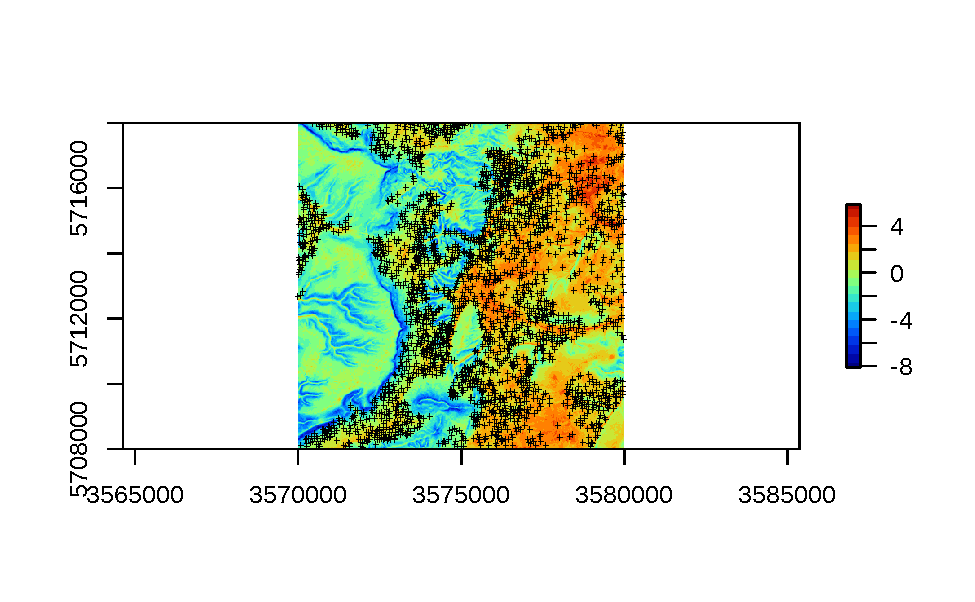
\includegraphics[width=0.9\linewidth]{resampling_files/figure-latex/eberg-allpnts-1} 

}

\caption{All sampling points available for Ebergotzen case study.}\label{fig:eberg-allpnts}
\end{figure}

If we ignore that property of the data and directly fit a predictive model for e.g.~
top-soil clay content using e.g.~random forest \citep{wright2017ranger} we get:

\begin{Shaded}
\begin{Highlighting}[]
\FunctionTok{library}\NormalTok{(ranger)}
\NormalTok{rm.eberg }\OtherTok{=} \FunctionTok{cbind}\NormalTok{(eberg[}\SpecialCharTok{!}\FunctionTok{is.na}\NormalTok{(ov.xy}\SpecialCharTok{$}\NormalTok{DEMTOPx),], sp}\SpecialCharTok{::}\FunctionTok{over}\NormalTok{(eberg.xy, eberg\_spc}\SpecialCharTok{@}\NormalTok{predicted))}
\NormalTok{cly.fm }\OtherTok{=} \FunctionTok{as.formula}\NormalTok{(}\FunctionTok{paste0}\NormalTok{(}\StringTok{"CLYMHT\_A \textasciitilde{} "}\NormalTok{, }\FunctionTok{paste0}\NormalTok{(}\StringTok{"PC"}\NormalTok{, }\DecValTok{1}\SpecialCharTok{:}\DecValTok{13}\NormalTok{, }\AttributeTok{collapse =} \StringTok{"+"}\NormalTok{)))}
\NormalTok{sel.cly }\OtherTok{=} \FunctionTok{complete.cases}\NormalTok{(rm.eberg[,}\FunctionTok{all.vars}\NormalTok{(cly.fm)])}
\NormalTok{rm.cly }\OtherTok{=}\NormalTok{ rm.eberg[sel.cly,]}
\NormalTok{rf.cly }\OtherTok{=}\NormalTok{ ranger}\SpecialCharTok{::}\FunctionTok{ranger}\NormalTok{(cly.fm, }\AttributeTok{data=}\NormalTok{rm.cly)}
\NormalTok{rf.cly}
\CommentTok{\#\textgreater{} Ranger result}
\CommentTok{\#\textgreater{} }
\CommentTok{\#\textgreater{} Call:}
\CommentTok{\#\textgreater{}  ranger::ranger(cly.fm, data = rm.cly) }
\CommentTok{\#\textgreater{} }
\CommentTok{\#\textgreater{} Type:                             Regression }
\CommentTok{\#\textgreater{} Number of trees:                  500 }
\CommentTok{\#\textgreater{} Sample size:                      2776 }
\CommentTok{\#\textgreater{} Number of independent variables:  13 }
\CommentTok{\#\textgreater{} Mtry:                             3 }
\CommentTok{\#\textgreater{} Target node size:                 5 }
\CommentTok{\#\textgreater{} Variable importance mode:         none }
\CommentTok{\#\textgreater{} Splitrule:                        variance }
\CommentTok{\#\textgreater{} OOB prediction error (MSE):       53.23538 }
\CommentTok{\#\textgreater{} R squared (OOB):                  0.6081801}
\end{Highlighting}
\end{Shaded}

This shows an RMSE of about 7.3\% and an R-square of about 0.61. The problem of this
accuracy measure is that with this Random Forest model we ignore spatial clustering
of points, hence both the model and the accuracy metric could be over-optimistic \citep{roberts2017cross, meyer2018improving}. Because we are typically interested in
how does the model perform over the WHOLE area of interest, not only in comparison
to out-of-bag points, we need to apply some adjustments to reduce overfitting or any bias in the BUPS.

Strategy \#1 for producing more objective estimate of model parameters is to
resample training points by forcing as much as possible equal sampling intensity
(hence mimicking the SRS), then observe performance of the model accuracy under
different resampling strategies. We can implement such spatial resampling using
the \texttt{sample.grid} function, which basically resamples the existing point samples
with an objective of producing a sample more similar to SRS. This type of
subsetting can be run \texttt{M} times and then an ensemble model can be produced in
which each individual model is based on spatially balanced samples. These are
not true SRS samples but we can refer to them as the \textbf{pseudo-SRS samples} as
they would probably pass most of the \textbf{Spatial Randomness tests}.

In R we can implement spatial resampling using the following three steps. First,
we generate e.g.~10 random subsets where the sampling intensity of points is
relatively homogeneous:

\begin{Shaded}
\begin{Highlighting}[]
\NormalTok{eberg.sp }\OtherTok{=} \FunctionTok{SpatialPointsDataFrame}\NormalTok{(eberg.xy, rm.eberg[}\FunctionTok{c}\NormalTok{(}\StringTok{"ID"}\NormalTok{,}\StringTok{"CLYMHT\_A"}\NormalTok{)])}
\NormalTok{sub.lst }\OtherTok{=} \FunctionTok{lapply}\NormalTok{(}\DecValTok{1}\SpecialCharTok{:}\DecValTok{10}\NormalTok{, }\ControlFlowTok{function}\NormalTok{(i)\{landmap}\SpecialCharTok{::}\FunctionTok{sample.grid}\NormalTok{(eberg.sp, }\FunctionTok{c}\NormalTok{(}\DecValTok{500}\NormalTok{, }\DecValTok{500}\NormalTok{), }\AttributeTok{n=}\DecValTok{2}\NormalTok{)\})}
\end{Highlighting}
\end{Shaded}

This randomly subsets each 500-m block to max 2 points i.e.~trims down the densely
sampled points to produce a relatively balanced spatial sampling intensity. We can
check that the training point sample looks more like a SRS or similar.

\begin{Shaded}
\begin{Highlighting}[]
\NormalTok{l1 }\OtherTok{\textless{}{-}} \FunctionTok{list}\NormalTok{(}\StringTok{"sp.points"}\NormalTok{, sub.lst[[}\DecValTok{1}\NormalTok{]]}\SpecialCharTok{$}\NormalTok{subset, }\AttributeTok{pch=}\StringTok{"+"}\NormalTok{, }\AttributeTok{col=}\StringTok{"black"}\NormalTok{)}
\FunctionTok{spplot}\NormalTok{(sub.lst[[}\DecValTok{1}\NormalTok{]]}\SpecialCharTok{$}\NormalTok{grid, }\AttributeTok{scales=}\FunctionTok{list}\NormalTok{(}\AttributeTok{draw=}\ConstantTok{TRUE}\NormalTok{),}
   \AttributeTok{col.regions=}\StringTok{"grey"}\NormalTok{, }\AttributeTok{sp.layout=}\FunctionTok{list}\NormalTok{(l1), }\AttributeTok{colorkey=}\ConstantTok{FALSE}\NormalTok{)}
\end{Highlighting}
\end{Shaded}

\begin{figure}

{\centering 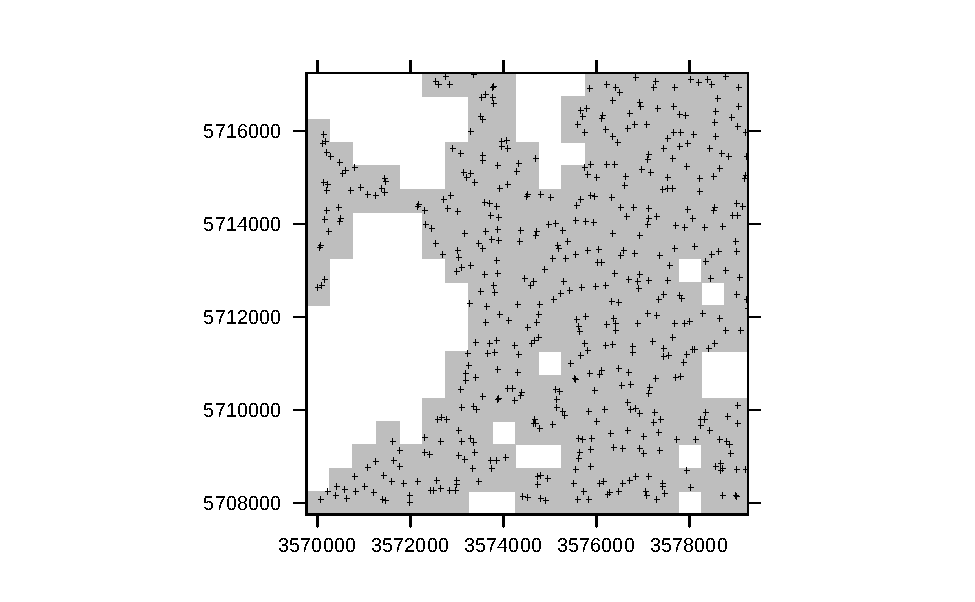
\includegraphics[width=0.9\linewidth]{resampling_files/figure-latex/eberg-grid-sample-1} 

}

\caption{Resampling original points using `sample.grid` function, which produces a sample with similar properties such as SRS.}\label{fig:eberg-grid-sample}
\end{figure}

Second, we can fit a list of random forest models using 10 random draws mimicking
some IID sampling:

\begin{Shaded}
\begin{Highlighting}[]
\NormalTok{rf.cly.lst }\OtherTok{=} \FunctionTok{lapply}\NormalTok{(}\DecValTok{1}\SpecialCharTok{:}\FunctionTok{length}\NormalTok{(sub.lst), }\ControlFlowTok{function}\NormalTok{(i)\{}
\NormalTok{        x }\OtherTok{\textless{}{-}}\NormalTok{ rm.eberg[}\FunctionTok{which}\NormalTok{(rm.eberg}\SpecialCharTok{$}\NormalTok{ID }\SpecialCharTok{\%in\%}\NormalTok{ sub.lst[[i]]}\SpecialCharTok{$}\NormalTok{subset}\SpecialCharTok{$}\NormalTok{ID),]; }
\NormalTok{        x }\OtherTok{\textless{}{-}}\NormalTok{ x[}\FunctionTok{complete.cases}\NormalTok{(x[,}\FunctionTok{all.vars}\NormalTok{(cly.fm)]),];}
\NormalTok{        y }\OtherTok{\textless{}{-}}\NormalTok{ ranger}\SpecialCharTok{::}\FunctionTok{ranger}\NormalTok{(cly.fm, }\AttributeTok{data=}\NormalTok{x, }\AttributeTok{num.trees =} \DecValTok{50}\NormalTok{); }
        \FunctionTok{return}\NormalTok{(y)}
\NormalTok{      \}}
\NormalTok{)}
\end{Highlighting}
\end{Shaded}

Third, we produce an Ensemble model that combines all predictions by simple
averaging \citep{wright2017ranger}. To produce final predictions, we can use
simple averaging because all subsets are symmetrical i.e.~have exactly the same
inputs and settings, hence all models fitted have equal importance for the ensemble model.

The out-of-bag accuracy of ranger now shows a somewhat higher RMSE, which is also
probably more realistic:

\begin{Shaded}
\begin{Highlighting}[]
\FunctionTok{mean}\NormalTok{(}\FunctionTok{sapply}\NormalTok{(rf.cly.lst, }\ControlFlowTok{function}\NormalTok{(i)\{}\FunctionTok{sqrt}\NormalTok{(i[[}\StringTok{"prediction.error"}\NormalTok{]])\}))}
\CommentTok{\#\textgreater{} [1] 8.003919}
\end{Highlighting}
\end{Shaded}

In summary, the actual error is most likely about 20\% higher than if we ignore
clustering and the previous model was likely over-optimistic. The model is too
much influenced by the clustered point samples and this should be taken into
account during model fitting \citep{roberts2017cross, meyer2021predicting}. If we
visually compare the predictions between the original and ensemble models we see:

\begin{Shaded}
\begin{Highlighting}[]
\NormalTok{cn }\OtherTok{=}\NormalTok{ rf.cly}\SpecialCharTok{$}\NormalTok{forest}\SpecialCharTok{$}\NormalTok{independent.variable.names}
\NormalTok{pred.cly }\OtherTok{=} \FunctionTok{predict}\NormalTok{(rf.cly, eberg\_spc}\SpecialCharTok{@}\NormalTok{predicted}\SpecialCharTok{@}\NormalTok{data[,cn])}
\NormalTok{eberg\_grid25}\SpecialCharTok{$}\NormalTok{pred.cly.rf }\OtherTok{=}\NormalTok{ pred.cly}\SpecialCharTok{$}\NormalTok{predictions}
\NormalTok{pred.cly.lst }\OtherTok{=} \FunctionTok{lapply}\NormalTok{(rf.cly.lst, }\ControlFlowTok{function}\NormalTok{(i)\{ }
    \FunctionTok{predict}\NormalTok{(i, eberg\_spc}\SpecialCharTok{@}\NormalTok{predicted}\SpecialCharTok{@}\NormalTok{data[,cn])}\SpecialCharTok{$}\NormalTok{predictions \})}
\NormalTok{eberg\_grid25}\SpecialCharTok{$}\NormalTok{pred.cly.erf }\OtherTok{=} \FunctionTok{rowMeans}\NormalTok{(}\FunctionTok{do.call}\NormalTok{(cbind, pred.cly.lst), }\AttributeTok{na.rm=}\ConstantTok{TRUE}\NormalTok{)}
\end{Highlighting}
\end{Shaded}

\begin{Shaded}
\begin{Highlighting}[]
\CommentTok{\#zlim.cly = quantile(rm.eberg$CLYMHT\_A, c(0.05, 0.95), na.rm=TRUE)}
\FunctionTok{spplot}\NormalTok{(eberg\_grid25[}\FunctionTok{c}\NormalTok{(}\StringTok{"pred.cly.rf"}\NormalTok{, }\StringTok{"pred.cly.erf"}\NormalTok{)], }\AttributeTok{col.regions=}\NormalTok{SAGA\_pal[[}\DecValTok{1}\NormalTok{]])}
\end{Highlighting}
\end{Shaded}

\begin{figure}

{\centering 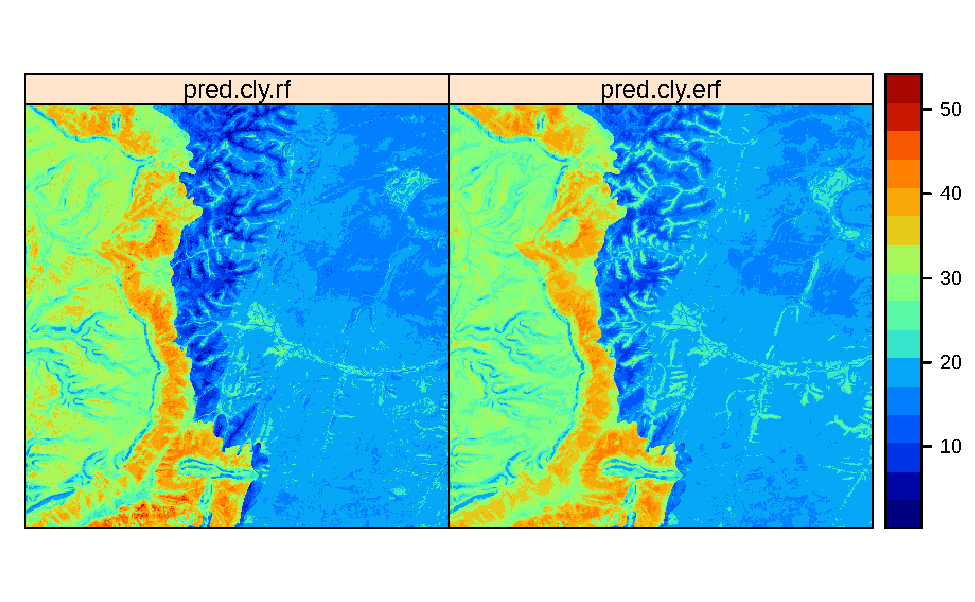
\includegraphics[width=0.9\linewidth]{resampling_files/figure-latex/eberg-pred-erf-1} 

}

\caption{Predictions of clay content: (left) ignoring spatial clustering effect on model, (right) after de-clustering of points.}\label{fig:eberg-pred-erf}
\end{figure}

Overall, the difference is small but there is certainly visible difference in predictions.
To the end users we would probably suggest to use \texttt{pred.cly.erf} (predictions produced
using the de-clustered points) map because the other model completely ignores
spatial clustering of points and this could have resulted in bias estimate of the
regression parameters. This solution to producing predictions is fully scalable
and relatively easy to implement, it only requires from user to decide on (1)
size of the block for subsampling, (2) max sampling intensity per block. In practice,
both could be determined by iterations.

\hypertarget{weighted-machine-learning}{%
\section{Weighted Machine Learning}\label{weighted-machine-learning}}

Note that the function \texttt{grid.sample} per definition draws points that are relatively
isolated (Fig. \ref{fig:eberg-fs}) with higher probability. We could implement a similar
principle but this time use the \texttt{case.weights} parameter approach (Strategy \#2). Many
Machine Learning algorithms allow for inclusion probabilities to be specified. For
example, we can instruct \texttt{ranger} to put more emphasis on isolated points / remove impact of
clustered points. The weighted estimation of model parameters is common in regression,
and also in spatial statistics (see e.g.~the \href{https://stat.ethz.ch/R-manual/R-devel/library/nlme/html/gls.html}{nlme::gls}; Generalized Least Square (GLS) function).
Theoretical basis for GLS / weighted regression is that the points that are clustered
might also be spatially correlated, and that means that they would introduce bias in
estimation of the regression parameters. Ideally, regression residuals should be
uncorrelated and uniform, hence a correction is needed that helps ensure these properties.

Weighted Machine Learning where bias in the sampling intensity is incorporated in
the modeling can be implemented in two steps. First, we derive the occurrence
probability (0--1) using the \texttt{spsample.prob} method:

\begin{Shaded}
\begin{Highlighting}[]
\NormalTok{iprob.all }\OtherTok{\textless{}{-}}\NormalTok{ landmap}\SpecialCharTok{::}\FunctionTok{spsample.prob}\NormalTok{(eberg.sp, eberg\_spc}\SpecialCharTok{@}\NormalTok{predicted[}\DecValTok{1}\SpecialCharTok{:}\DecValTok{4}\NormalTok{])}
\CommentTok{\#\textgreater{} Deriving kernel density map using sigma 157 ...}
\CommentTok{\#\textgreater{} Deriving inclusion probabilities using MaxLike analysis...}
\end{Highlighting}
\end{Shaded}

\begin{Shaded}
\begin{Highlighting}[]
\FunctionTok{plot}\NormalTok{(}\FunctionTok{raster}\NormalTok{(iprob.all}\SpecialCharTok{$}\NormalTok{prob), }\AttributeTok{zlim=}\FunctionTok{c}\NormalTok{(}\DecValTok{0}\NormalTok{,}\DecValTok{1}\NormalTok{))}
\FunctionTok{points}\NormalTok{(iprob.all}\SpecialCharTok{$}\NormalTok{observations, }\AttributeTok{pch=}\StringTok{"+"}\NormalTok{, }\AttributeTok{cex=}\NormalTok{.}\DecValTok{5}\NormalTok{)}
\end{Highlighting}
\end{Shaded}

\begin{figure}

{\centering 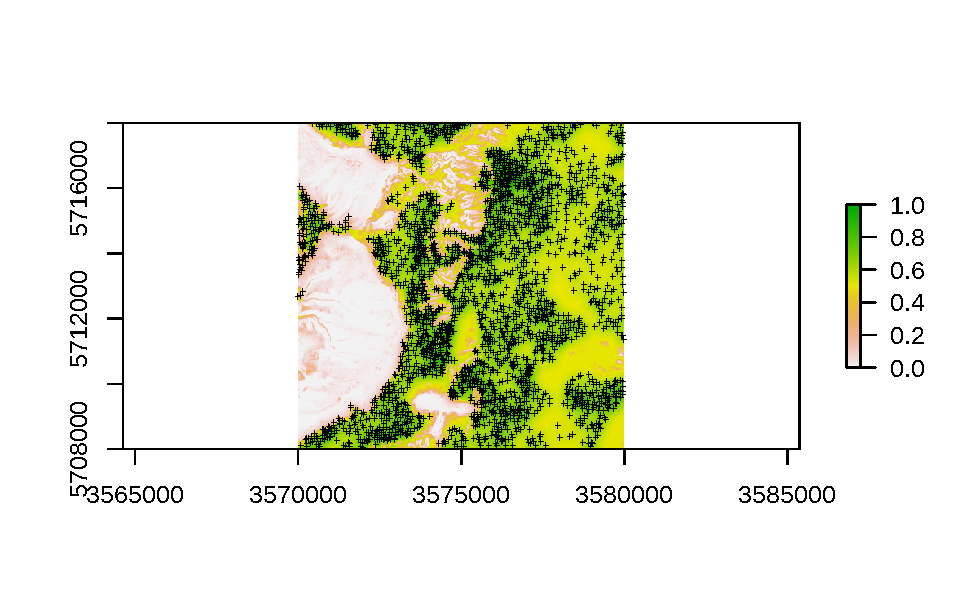
\includegraphics[width=0.9\linewidth]{resampling_files/figure-latex/eberg-iprob-1} 

}

\caption{Occurrence probability for existing point samples for the Ebergotzen case study derived as an average between the kernel density and maxlike occurrence probabilities.}\label{fig:eberg-iprob}
\end{figure}

Second, we fit a model using all points, but this time we set \texttt{case.weights} to be
reversely proportional to probability of occurrence (hence points with lower occurrence
probability get higher weights):

\begin{Shaded}
\begin{Highlighting}[]
\NormalTok{ov.weigths }\OtherTok{=} \DecValTok{1}\SpecialCharTok{/}\NormalTok{sp}\SpecialCharTok{::}\FunctionTok{over}\NormalTok{(eberg.xy, iprob.all}\SpecialCharTok{$}\NormalTok{prob)[]}
\NormalTok{rf.clyI }\OtherTok{=}\NormalTok{ ranger}\SpecialCharTok{::}\FunctionTok{ranger}\NormalTok{(cly.fm, }\AttributeTok{data=}\NormalTok{rm.cly, }\AttributeTok{case.weights =}\NormalTok{ ov.weigths[sel.cly,])}
\end{Highlighting}
\end{Shaded}

\href{https://www.statology.org/weighted-least-squares-in-r/}{Weighted regression} is a common technique in statistics and in this case the weights are used to helps reduce
clustering effect i.e.~give weights to points proportionally to the sampling bias.
This method is in principle similar to the \href{https://stat.ethz.ch/R-manual/R-devel/library/nlme/html/gls.html}{nlme::gls} Generalized Least Square (GLS) procedure,
but with the difference that we do not estimate any spatial autocorrelation structure, but
instead incorporate the probability of occurrence to reduce effect of spatial clustering.

\hypertarget{resampling-using-ensemble-ml}{%
\section{Resampling using Ensemble ML}\label{resampling-using-ensemble-ml}}

Another approach to improve generating BUPS from clustered point data is to switch
to Ensemble ML i.e.~use a multitude of ML methods (so called \textbf{base-learners}),
then estimate final predictions using robust resampling and blocking. Ensemble ML
has shown to help increase mapping accuracy, but also helps with reducing \emph{over-shooting}
effects due to \href{https://medium.com/nerd-for-tech/extrapolation-is-tough-for-trees-tree-based-learners-combining-learners-of-different-type-makes-659187a6f58d}{extrapolation}.

One way to reduce effects of point clustering for predictive is to use \emph{spatial blocking}
i.e.~to make sure that spatially clustered points are not used both for training and
internal validation \citep{roberts2017cross}. First, we need to define a spatial grid that we will use
as a blocking parameter. We set here arbitrarily size of spatial blocks to 500-m,
in practice the block size can be determined more objectively by e.g.~analyzing
at which distances is clustering reduced:

\begin{Shaded}
\begin{Highlighting}[]
\NormalTok{grd }\OtherTok{\textless{}{-}}\NormalTok{ sp}\SpecialCharTok{::}\FunctionTok{GridTopology}\NormalTok{(}\AttributeTok{cellcentre.offset=}\NormalTok{eberg\_grid25}\SpecialCharTok{@}\NormalTok{bbox[,}\DecValTok{1}\NormalTok{], }\AttributeTok{cellsize=}\FunctionTok{rep}\NormalTok{(}\DecValTok{500}\NormalTok{,}\DecValTok{2}\NormalTok{),}
                        \AttributeTok{cells.dim=}\FunctionTok{c}\NormalTok{(}\FunctionTok{ceiling}\NormalTok{(}\FunctionTok{abs}\NormalTok{(}\FunctionTok{diff}\NormalTok{(eberg\_grid25}\SpecialCharTok{@}\NormalTok{bbox[}\DecValTok{1}\NormalTok{,])}\SpecialCharTok{/}\DecValTok{500}\NormalTok{))}\SpecialCharTok{+}\DecValTok{1}\NormalTok{,}
                        \FunctionTok{ceiling}\NormalTok{(}\FunctionTok{abs}\NormalTok{(}\FunctionTok{diff}\NormalTok{(eberg\_grid25}\SpecialCharTok{@}\NormalTok{bbox[}\DecValTok{2}\NormalTok{,])}\SpecialCharTok{/}\DecValTok{500}\NormalTok{))}\SpecialCharTok{+}\DecValTok{1}\NormalTok{))}
\NormalTok{r.sp }\OtherTok{\textless{}{-}}\NormalTok{ sp}\SpecialCharTok{::}\FunctionTok{SpatialGridDataFrame}\NormalTok{(grd, }\AttributeTok{proj4string =}\NormalTok{ eberg\_grid25}\SpecialCharTok{@}\NormalTok{proj4string,}
                    \AttributeTok{data=}\FunctionTok{data.frame}\NormalTok{(}\AttributeTok{gid=}\DecValTok{1}\SpecialCharTok{:}\NormalTok{(grd}\SpecialCharTok{@}\NormalTok{cells.dim[}\DecValTok{1}\NormalTok{] }\SpecialCharTok{*}\NormalTok{ grd}\SpecialCharTok{@}\NormalTok{cells.dim[}\DecValTok{2}\NormalTok{])))}
\NormalTok{id }\OtherTok{\textless{}{-}}\NormalTok{ sp}\SpecialCharTok{::}\FunctionTok{over}\NormalTok{(eberg.xy, r.sp)}\SpecialCharTok{$}\NormalTok{gid}
\CommentTok{\#summary(as.factor(id))}
\end{Highlighting}
\end{Shaded}

\begin{Shaded}
\begin{Highlighting}[]
\FunctionTok{plot}\NormalTok{(r.sp)}
\FunctionTok{points}\NormalTok{(eberg.xy, }\AttributeTok{pch=}\StringTok{"+"}\NormalTok{, }\AttributeTok{cex=}\NormalTok{.}\DecValTok{5}\NormalTok{)}
\end{Highlighting}
\end{Shaded}

\begin{figure}

{\centering 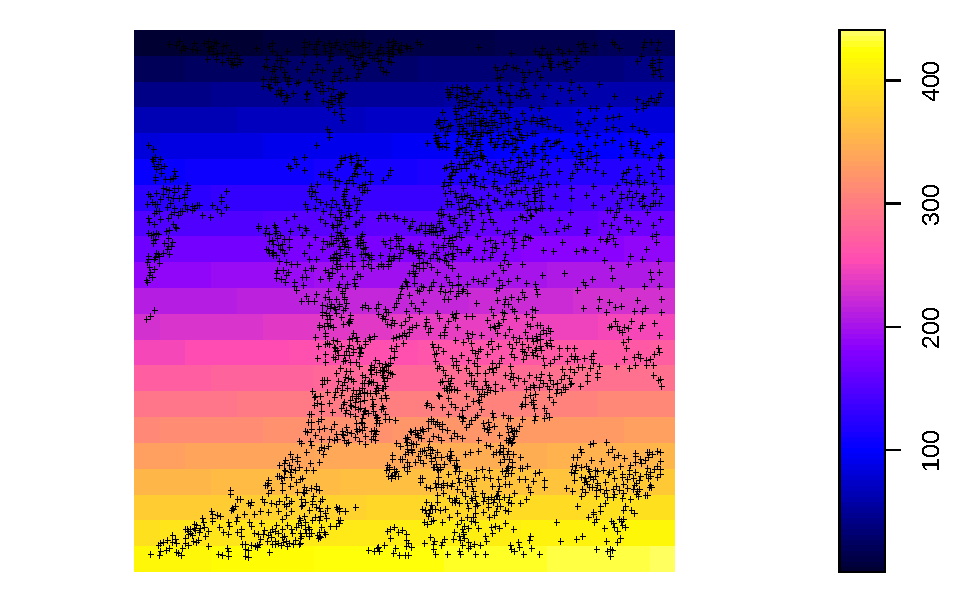
\includegraphics[width=0.9\linewidth]{resampling_files/figure-latex/eberg-grid-1} 

}

\caption{500 m grid for spatial resampling.}\label{fig:eberg-grid}
\end{figure}

This shows that many blocks basically have no training points, and some blocks
are densely sampled with e.g.~15--20 points. Next, we can compare models fitted
using spatial blocking vs no special settings. First, we fit ensemble ML model using no blocking:

\begin{Shaded}
\begin{Highlighting}[]
\NormalTok{parallelMap}\SpecialCharTok{::}\FunctionTok{parallelStartSocket}\NormalTok{(parallel}\SpecialCharTok{::}\FunctionTok{detectCores}\NormalTok{())}
\CommentTok{\#\textgreater{} Starting parallelization in mode=socket with cpus=32.}
\end{Highlighting}
\end{Shaded}

\begin{Shaded}
\begin{Highlighting}[]
\FunctionTok{library}\NormalTok{(mlr)}
\FunctionTok{library}\NormalTok{(glmnet)}
\FunctionTok{library}\NormalTok{(Cubist)}
\NormalTok{lrns }\OtherTok{\textless{}{-}} \FunctionTok{list}\NormalTok{(mlr}\SpecialCharTok{::}\FunctionTok{makeLearner}\NormalTok{(}\StringTok{"regr.ranger"}\NormalTok{, }
                \AttributeTok{num.threads =}\NormalTok{ parallel}\SpecialCharTok{::}\FunctionTok{detectCores}\NormalTok{(), }\AttributeTok{num.trees=}\DecValTok{150}\NormalTok{, }\AttributeTok{importance=}\StringTok{"impurity"}\NormalTok{),}
\NormalTok{             mlr}\SpecialCharTok{::}\FunctionTok{makeLearner}\NormalTok{(}\StringTok{"regr.glm"}\NormalTok{), mlr}\SpecialCharTok{::}\FunctionTok{makeLearner}\NormalTok{(}\StringTok{"regr.cubist"}\NormalTok{),}
\NormalTok{             mlr}\SpecialCharTok{::}\FunctionTok{makeLearner}\NormalTok{(}\StringTok{"regr.cvglmnet"}\NormalTok{))}
\NormalTok{tsk0 }\OtherTok{\textless{}{-}}\NormalTok{ mlr}\SpecialCharTok{::}\FunctionTok{makeRegrTask}\NormalTok{(}\AttributeTok{data =}\NormalTok{ rm.cly[,}\FunctionTok{all.vars}\NormalTok{(cly.fm)], }\AttributeTok{target =} \StringTok{"CLYMHT\_A"}\NormalTok{)}
\NormalTok{init0.m }\OtherTok{\textless{}{-}}\NormalTok{ mlr}\SpecialCharTok{::}\FunctionTok{makeStackedLearner}\NormalTok{(lrns, }\AttributeTok{method =} \StringTok{"stack.cv"}\NormalTok{, }
                                  \AttributeTok{super.learner =} \StringTok{"regr.lm"}\NormalTok{,}
                                  \AttributeTok{resampling=}\NormalTok{mlr}\SpecialCharTok{::}\FunctionTok{makeResampleDesc}\NormalTok{(}\AttributeTok{method =} \StringTok{"CV"}\NormalTok{))}
\NormalTok{eml0 }\OtherTok{=} \FunctionTok{train}\NormalTok{(init0.m, tsk0)}
\CommentTok{\#\textgreater{} Exporting objects to slaves for mode socket: .mlr.slave.options}
\CommentTok{\#\textgreater{} Mapping in parallel: mode = socket; level = mlr.resample; cpus = 32; elements = 10.}
\CommentTok{\#\textgreater{} Exporting objects to slaves for mode socket: .mlr.slave.options}
\CommentTok{\#\textgreater{} Mapping in parallel: mode = socket; level = mlr.resample; cpus = 32; elements = 10.}
\CommentTok{\#\textgreater{} Exporting objects to slaves for mode socket: .mlr.slave.options}
\CommentTok{\#\textgreater{} Mapping in parallel: mode = socket; level = mlr.resample; cpus = 32; elements = 10.}
\CommentTok{\#\textgreater{} Exporting objects to slaves for mode socket: .mlr.slave.options}
\CommentTok{\#\textgreater{} Mapping in parallel: mode = socket; level = mlr.resample; cpus = 32; elements = 10.}
\FunctionTok{summary}\NormalTok{(eml0}\SpecialCharTok{$}\NormalTok{learner.model}\SpecialCharTok{$}\NormalTok{super.model}\SpecialCharTok{$}\NormalTok{learner.model)}
\CommentTok{\#\textgreater{} }
\CommentTok{\#\textgreater{} Call:}
\CommentTok{\#\textgreater{} stats::lm(formula = f, data = d)}
\CommentTok{\#\textgreater{} }
\CommentTok{\#\textgreater{} Residuals:}
\CommentTok{\#\textgreater{}     Min      1Q  Median      3Q     Max }
\CommentTok{\#\textgreater{} {-}33.228  {-}4.005   0.298   3.054  37.818 }
\CommentTok{\#\textgreater{} }
\CommentTok{\#\textgreater{} Coefficients:}
\CommentTok{\#\textgreater{}               Estimate Std. Error t value Pr(\textgreater{}|t|)    }
\CommentTok{\#\textgreater{} (Intercept)   {-}0.55143    0.47112  {-}1.170 0.241906    }
\CommentTok{\#\textgreater{} regr.ranger    0.80513    0.05689  14.152  \textless{} 2e{-}16 ***}
\CommentTok{\#\textgreater{} regr.glm       0.24905    0.11067   2.250 0.024502 *  }
\CommentTok{\#\textgreater{} regr.cubist    0.13973    0.04208   3.320 0.000911 ***}
\CommentTok{\#\textgreater{} regr.cvglmnet {-}0.17004    0.11544  {-}1.473 0.140868    }
\CommentTok{\#\textgreater{} {-}{-}{-}}
\CommentTok{\#\textgreater{} Signif. codes:  0 \textquotesingle{}***\textquotesingle{} 0.001 \textquotesingle{}**\textquotesingle{} 0.01 \textquotesingle{}*\textquotesingle{} 0.05 \textquotesingle{}.\textquotesingle{} 0.1 \textquotesingle{} \textquotesingle{} 1}
\CommentTok{\#\textgreater{} }
\CommentTok{\#\textgreater{} Residual standard error: 7.339 on 2771 degrees of freedom}
\CommentTok{\#\textgreater{} Multiple R{-}squared:  0.6041, Adjusted R{-}squared:  0.6036 }
\CommentTok{\#\textgreater{} F{-}statistic:  1057 on 4 and 2771 DF,  p{-}value: \textless{} 2.2e{-}16}
\end{Highlighting}
\end{Shaded}

This shows that \texttt{ranger} i.e.~random forest and \texttt{cubist} are the most important
learners and the overall model performance matches the previously fitted model using ranger.
Next, we fit an ensemble ML model with the spatial blocking (500-m):

\begin{Shaded}
\begin{Highlighting}[]
\NormalTok{tsk1 }\OtherTok{\textless{}{-}}\NormalTok{ mlr}\SpecialCharTok{::}\FunctionTok{makeRegrTask}\NormalTok{(}\AttributeTok{data =}\NormalTok{ rm.cly[,}\FunctionTok{all.vars}\NormalTok{(cly.fm)], }\AttributeTok{target =} \StringTok{"CLYMHT\_A"}\NormalTok{, }
                          \AttributeTok{blocking =} \FunctionTok{as.factor}\NormalTok{(id[sel.cly]))}
\NormalTok{init1.m }\OtherTok{\textless{}{-}}\NormalTok{ mlr}\SpecialCharTok{::}\FunctionTok{makeStackedLearner}\NormalTok{(lrns, }\AttributeTok{method =} \StringTok{"stack.cv"}\NormalTok{, }
                  \AttributeTok{super.learner =} \StringTok{"regr.lm"}\NormalTok{,}
                  \AttributeTok{resampling=}\NormalTok{mlr}\SpecialCharTok{::}\FunctionTok{makeResampleDesc}\NormalTok{(}\AttributeTok{method =} \StringTok{"CV"}\NormalTok{, }\AttributeTok{blocking.cv=}\ConstantTok{TRUE}\NormalTok{))}
\NormalTok{eml1 }\OtherTok{=} \FunctionTok{train}\NormalTok{(init1.m, tsk1)}
\CommentTok{\#\textgreater{} Exporting objects to slaves for mode socket: .mlr.slave.options}
\CommentTok{\#\textgreater{} Mapping in parallel: mode = socket; level = mlr.resample; cpus = 32; elements = 10.}
\CommentTok{\#\textgreater{} Exporting objects to slaves for mode socket: .mlr.slave.options}
\CommentTok{\#\textgreater{} Mapping in parallel: mode = socket; level = mlr.resample; cpus = 32; elements = 10.}
\CommentTok{\#\textgreater{} Exporting objects to slaves for mode socket: .mlr.slave.options}
\CommentTok{\#\textgreater{} Mapping in parallel: mode = socket; level = mlr.resample; cpus = 32; elements = 10.}
\CommentTok{\#\textgreater{} Exporting objects to slaves for mode socket: .mlr.slave.options}
\CommentTok{\#\textgreater{} Mapping in parallel: mode = socket; level = mlr.resample; cpus = 32; elements = 10.}
\FunctionTok{summary}\NormalTok{(eml1}\SpecialCharTok{$}\NormalTok{learner.model}\SpecialCharTok{$}\NormalTok{super.model}\SpecialCharTok{$}\NormalTok{learner.model)}
\CommentTok{\#\textgreater{} }
\CommentTok{\#\textgreater{} Call:}
\CommentTok{\#\textgreater{} stats::lm(formula = f, data = d)}
\CommentTok{\#\textgreater{} }
\CommentTok{\#\textgreater{} Residuals:}
\CommentTok{\#\textgreater{}     Min      1Q  Median      3Q     Max }
\CommentTok{\#\textgreater{} {-}31.676  {-}4.201   0.443   3.109  40.386 }
\CommentTok{\#\textgreater{} }
\CommentTok{\#\textgreater{} Coefficients:}
\CommentTok{\#\textgreater{}               Estimate Std. Error t value Pr(\textgreater{}|t|)    }
\CommentTok{\#\textgreater{} (Intercept)   {-}0.36065    0.48143  {-}0.749   0.4539    }
\CommentTok{\#\textgreater{} regr.ranger    0.63875    0.05688  11.229  \textless{} 2e{-}16 ***}
\CommentTok{\#\textgreater{} regr.glm       0.21547    0.11185   1.926   0.0542 .  }
\CommentTok{\#\textgreater{} regr.cubist    0.23915    0.04124   5.800  7.4e{-}09 ***}
\CommentTok{\#\textgreater{} regr.cvglmnet {-}0.08255    0.11581  {-}0.713   0.4760    }
\CommentTok{\#\textgreater{} {-}{-}{-}}
\CommentTok{\#\textgreater{} Signif. codes:  0 \textquotesingle{}***\textquotesingle{} 0.001 \textquotesingle{}**\textquotesingle{} 0.01 \textquotesingle{}*\textquotesingle{} 0.05 \textquotesingle{}.\textquotesingle{} 0.1 \textquotesingle{} \textquotesingle{} 1}
\CommentTok{\#\textgreater{} }
\CommentTok{\#\textgreater{} Residual standard error: 7.514 on 2771 degrees of freedom}
\CommentTok{\#\textgreater{} Multiple R{-}squared:  0.5851, Adjusted R{-}squared:  0.5845 }
\CommentTok{\#\textgreater{} F{-}statistic: 976.9 on 4 and 2771 DF,  p{-}value: \textless{} 2.2e{-}16}
\end{Highlighting}
\end{Shaded}

which shows a difference: the RMSE drops for 10--20\% and the \texttt{regr.glm} learner is
now also significant. In the previous example, it is possible that the \texttt{regr.glm} model
was possibly \emph{shadowed} by the fitting power of ranger and Cubist, while after
more strict CV, also more simple models seem to perform with a comparable accuracy.

We can produce predictions using the Ensemble ML model developed with blocking by running:

\begin{Shaded}
\begin{Highlighting}[]
\NormalTok{pred.cly.eml }\OtherTok{=} \FunctionTok{predict}\NormalTok{(eml1, }\AttributeTok{newdata=}\NormalTok{eberg\_spc}\SpecialCharTok{@}\NormalTok{predicted}\SpecialCharTok{@}\NormalTok{data[,eml1}\SpecialCharTok{$}\NormalTok{features])}
\NormalTok{eberg\_grid25}\SpecialCharTok{$}\NormalTok{pred.cly.eml }\OtherTok{=}\NormalTok{ pred.cly.eml}\SpecialCharTok{$}\NormalTok{data}\SpecialCharTok{$}\NormalTok{response}
\end{Highlighting}
\end{Shaded}

\begin{Shaded}
\begin{Highlighting}[]
\FunctionTok{spplot}\NormalTok{(eberg\_grid25[}\FunctionTok{c}\NormalTok{(}\StringTok{"pred.cly.eml"}\NormalTok{, }\StringTok{"pred.cly.erf"}\NormalTok{)], }\AttributeTok{col.regions=}\NormalTok{SAGA\_pal[[}\DecValTok{1}\NormalTok{]])}
\end{Highlighting}
\end{Shaded}

\begin{figure}

{\centering 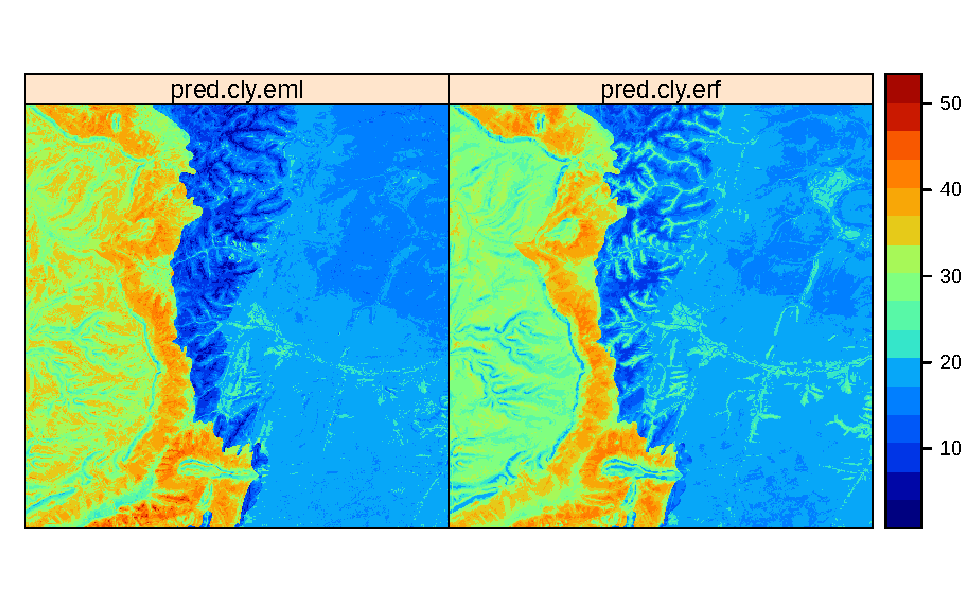
\includegraphics[width=0.9\linewidth]{resampling_files/figure-latex/eberg-eml-1} 

}

\caption{Predictions of clay content: (left) Ensemble ML with spatial blocking, (right) after de-clustring of points.}\label{fig:eberg-eml}
\end{figure}

Visual comparison with the predictions produced in previous section, show that
the Ensemble method \texttt{pred.cly.eml} predicts somewhat higher clay content in the
extrapolation area, but also smooths out some higher values in the plains.
Again, if we have to choose we would suggest users to use the map on the left for
two main reasons:

\begin{enumerate}
\def\labelenumi{\arabic{enumi}.}
\tightlist
\item
  It is based on multiple base-learners, not only on Random Forest and results
  show that both Cubist and glmnet package produce comparable results to RF.\\
\item
  It is probably more sensible to use the predictions produced by the meta-learner,
  especially in the extrapolation space.
\end{enumerate}

\hypertarget{estimating-the-area-of-applicability}{%
\section{Estimating the Area of Applicability}\label{estimating-the-area-of-applicability}}

\citet{meyer2021predicting} have developed a method to estimate so-called \href{https://cran.r-project.org/web/packages/CAST/vignettes/AOA-tutorial.html}{``Area of Applicability''}
using a fitted model and feature space analysis. This method can be used for
post-modeling analysis and helps users realize what are the true extrapolation
areas and where the predictions are critically poor. The users can then choose to
e.g.~limit predictions only to combinations of pixels that are NOT too risky (extrapolation).

For the RF model fitted above we can derive AoA using:

\begin{Shaded}
\begin{Highlighting}[]
\FunctionTok{library}\NormalTok{(CAST)}
\NormalTok{train.df }\OtherTok{=}\NormalTok{ rm.cly[,}\FunctionTok{all.vars}\NormalTok{(cly.fm)[}\SpecialCharTok{{-}}\DecValTok{1}\NormalTok{]]}
\NormalTok{weight }\OtherTok{=} \FunctionTok{as.data.frame}\NormalTok{(mlr}\SpecialCharTok{::}\FunctionTok{getFeatureImportance}\NormalTok{(eml1}\SpecialCharTok{$}\NormalTok{learner.model}\SpecialCharTok{$}\NormalTok{base.models[[}\DecValTok{1}\NormalTok{]])}\SpecialCharTok{$}\NormalTok{res)}
\NormalTok{AOA }\OtherTok{\textless{}{-}}\NormalTok{ CAST}\SpecialCharTok{::}\FunctionTok{aoa}\NormalTok{(}\AttributeTok{train=}\NormalTok{train.df, }\AttributeTok{predictors=}\NormalTok{eberg\_spc}\SpecialCharTok{@}\NormalTok{predicted}\SpecialCharTok{@}\NormalTok{data[,eml1}\SpecialCharTok{$}\NormalTok{features], }\AttributeTok{weight=}\NormalTok{weight)}
\end{Highlighting}
\end{Shaded}

This method can be computational so it is probably not recommended for larger datasets.
Some examples of the Area of Applicability can be found in the \href{https://cran.r-project.org/web/packages/CAST/vignettes/AOA-tutorial.html}{CAST package tutorial}.

\hypertarget{estimating-per-pixel-mapping-accuracy}{%
\section{Estimating per-pixel mapping accuracy}\label{estimating-per-pixel-mapping-accuracy}}

Using the Ensemble Model we can also estimate the mapping accuracy per pixel i.e.~
by deriving the \textbf{Mean Square Prediction Error} (MSPE). The \textbf{forestError} package currently
provides a \emph{``Unified Framework for Random Forest Prediction Error Estimation''} \citep{lu2021unified}
and is probably the most worked-out procedure for deriving prediction errors
and estimating potential bias. This requires two steps, (1) first, we need to
fit an additional quantile Regression RF model (using the four base learners from the
previous section), (2) second, we can then estimate complete error statistics
per pixel using the \href{https://rdrr.io/cran/forestError/man/quantForestError.html}{quantForestError} function.

Because derivation of prediction errors per pixel can often be computational
(even at the order of magnitude more computational than predictions), it is important
to use a method that is computationally efficient and precise enough. In the
landmap package the uncertainty is derived using base learners instead of using
ALL raster layers which could be hundreds. This approach of using (few) base learners
instead of (many) original covariates helps compress the complexity of model and
significantly speed-up computing. The base learners can be accessed from the
mlr object:

\begin{Shaded}
\begin{Highlighting}[]
\NormalTok{eml.t }\OtherTok{=}\NormalTok{ eml1}\SpecialCharTok{$}\NormalTok{learner.model}\SpecialCharTok{$}\NormalTok{super.model}\SpecialCharTok{$}\NormalTok{learner.model}\SpecialCharTok{$}\NormalTok{terms}
\FunctionTok{paste}\NormalTok{(eml.t)}
\CommentTok{\#\textgreater{} [1] "\textasciitilde{}"                                                   }
\CommentTok{\#\textgreater{} [2] "CLYMHT\_A"                                            }
\CommentTok{\#\textgreater{} [3] "regr.ranger + regr.glm + regr.cubist + regr.cvglmnet"}
\NormalTok{eml.m }\OtherTok{=}\NormalTok{ eml1}\SpecialCharTok{$}\NormalTok{learner.model}\SpecialCharTok{$}\NormalTok{super.model}\SpecialCharTok{$}\NormalTok{learner.model}\SpecialCharTok{$}\NormalTok{model}
\end{Highlighting}
\end{Shaded}

We use the spatially resampled base-learners to fit (an independent) quantile RF:

\begin{Shaded}
\begin{Highlighting}[]
\NormalTok{eml.qr }\OtherTok{\textless{}{-}}\NormalTok{ ranger}\SpecialCharTok{::}\FunctionTok{ranger}\NormalTok{(eml.t, eml.m, }\AttributeTok{num.trees=}\DecValTok{85}\NormalTok{, }\AttributeTok{importance=}\StringTok{"impurity"}\NormalTok{, }
                         \AttributeTok{quantreg=}\ConstantTok{TRUE}\NormalTok{, }\AttributeTok{keep.inbag =} \ConstantTok{TRUE}\NormalTok{)}
\CommentTok{\#eml.qr}
\end{Highlighting}
\end{Shaded}

Next, we can use the \texttt{forestError} package to derive prediction errors by:

\begin{Shaded}
\begin{Highlighting}[]
\FunctionTok{library}\NormalTok{(forestError)}
\NormalTok{quantiles }\OtherTok{=} \FunctionTok{c}\NormalTok{((}\DecValTok{1}\FloatTok{{-}.682}\NormalTok{)}\SpecialCharTok{/}\DecValTok{2}\NormalTok{, }\DecValTok{1}\SpecialCharTok{{-}}\NormalTok{(}\DecValTok{1}\FloatTok{{-}.682}\NormalTok{)}\SpecialCharTok{/}\DecValTok{2}\NormalTok{)}
\NormalTok{n.cores }\OtherTok{=}\NormalTok{ parallel}\SpecialCharTok{::}\FunctionTok{detectCores}\NormalTok{()}
\NormalTok{out.c }\OtherTok{\textless{}{-}} \FunctionTok{as.data.frame}\NormalTok{(mlr}\SpecialCharTok{::}\FunctionTok{getStackedBaseLearnerPredictions}\NormalTok{(eml1, }
          \AttributeTok{newdata=}\NormalTok{eberg\_spc}\SpecialCharTok{@}\NormalTok{predicted}\SpecialCharTok{@}\NormalTok{data[,eml1}\SpecialCharTok{$}\NormalTok{features]))}
\NormalTok{pred.q }\OtherTok{=}\NormalTok{ forestError}\SpecialCharTok{::}\FunctionTok{quantForestError}\NormalTok{(eml.qr, }
                    \AttributeTok{X.train =}\NormalTok{ eml.m[,}\FunctionTok{all.vars}\NormalTok{(eml.t)[}\SpecialCharTok{{-}}\DecValTok{1}\NormalTok{]], }
                    \AttributeTok{X.test =}\NormalTok{ out.c, }
                    \AttributeTok{Y.train =}\NormalTok{ eml.m[,}\FunctionTok{all.vars}\NormalTok{(eml.t)[}\DecValTok{1}\NormalTok{]], }
                    \AttributeTok{alpha =}\NormalTok{ (}\DecValTok{1}\SpecialCharTok{{-}}\NormalTok{(quantiles[}\DecValTok{2}\NormalTok{]}\SpecialCharTok{{-}}\NormalTok{quantiles[}\DecValTok{1}\NormalTok{])), }\AttributeTok{n.cores=}\NormalTok{n.cores)}
\end{Highlighting}
\end{Shaded}

We could have also subset e.g.~10\% of the input points and keep them ONLY for
estimating the prediction errors using the \texttt{quantForestError}, which is also
recommended by the authors of the forestError package. In practice, because
base learners have been fitted using 5-fold Cross-Validation with blocking,
they are already out-of-bag samples hence taking out extra OOB samples is
probably not required, but you can also test this with your own data.

The \texttt{quantForestError} function runs a complete uncertainty assessment and
includes both MSPE, bias and upper and lower confidence intervals:

\begin{Shaded}
\begin{Highlighting}[]
\FunctionTok{str}\NormalTok{(pred.q)}
\CommentTok{\#\textgreater{} List of 3}
\CommentTok{\#\textgreater{}  $ estimates:\textquotesingle{}data.frame\textquotesingle{}:   160000 obs. of  5 variables:}
\CommentTok{\#\textgreater{}   ..$ pred       : num [1:160000] 35.2 37.5 31.7 36 35.9 ...}
\CommentTok{\#\textgreater{}   ..$ mspe       : num [1:160000] 138.1 104.1 82.7 90.9 76.2 ...}
\CommentTok{\#\textgreater{}   ..$ bias       : num [1:160000] {-}1.77 {-}1.22 {-}1.13 {-}1.18 {-}1.45 ...}
\CommentTok{\#\textgreater{}   ..$ lower\_0.318: num [1:160000] 23.5 27.8 21.5 29.6 29.5 ...}
\CommentTok{\#\textgreater{}   ..$ upper\_0.318: num [1:160000] 52.7 47.7 40.2 47.7 42.3 ...}
\CommentTok{\#\textgreater{}  $ perror   :function (q, xs = 1:n.test)  }
\CommentTok{\#\textgreater{}  $ qerror   :function (p, xs = 1:n.test)}
\end{Highlighting}
\end{Shaded}

In this case, for the lower and upper confidence intervals we use 1-standard
deviation probability which is about 2/3 probability and hence the lower value is 0.159
and upper 0.841. The RMSPE should match the half of the difference between
the lower and upper interval in this case, although there will be difference in exact numbers.

The mean RMSPE for the whole study area (mean of all pixels) should be as expected
somewhat higher than the RMSE we get from model fitting:

\begin{Shaded}
\begin{Highlighting}[]
\FunctionTok{mean}\NormalTok{(}\FunctionTok{sqrt}\NormalTok{(pred.q}\SpecialCharTok{$}\NormalTok{estimates}\SpecialCharTok{$}\NormalTok{mspe), }\AttributeTok{na.rm=}\ConstantTok{TRUE}\NormalTok{)}
\CommentTok{\#\textgreater{} [1] 7.780946}
\end{Highlighting}
\end{Shaded}

This is because we are also extrapolating in the large part of the area.
The map in Fig. \ref{fig:eberg-var-eml} correctly depicts the extrapolation areas
as having much higher RMSPE (compare with Fig. \ref{fig:eberg-iprob}):

\begin{Shaded}
\begin{Highlighting}[]
\NormalTok{eberg\_grid25}\SpecialCharTok{$}\NormalTok{rmspe.cly.eml }\OtherTok{=} \FunctionTok{sqrt}\NormalTok{(pred.q}\SpecialCharTok{$}\NormalTok{estimates}\SpecialCharTok{$}\NormalTok{mspe)}
\FunctionTok{plot}\NormalTok{(}\FunctionTok{raster}\NormalTok{(eberg\_grid25[}\FunctionTok{c}\NormalTok{(}\StringTok{"rmspe.cly.eml"}\NormalTok{)]), }\AttributeTok{col=}\NormalTok{SAGA\_pal[[}\DecValTok{16}\NormalTok{]])}
\FunctionTok{points}\NormalTok{(eberg.sp, }\AttributeTok{pch=}\StringTok{"+"}\NormalTok{, }\AttributeTok{cex=}\NormalTok{.}\DecValTok{6}\NormalTok{)}
\end{Highlighting}
\end{Shaded}

\begin{figure}

{\centering 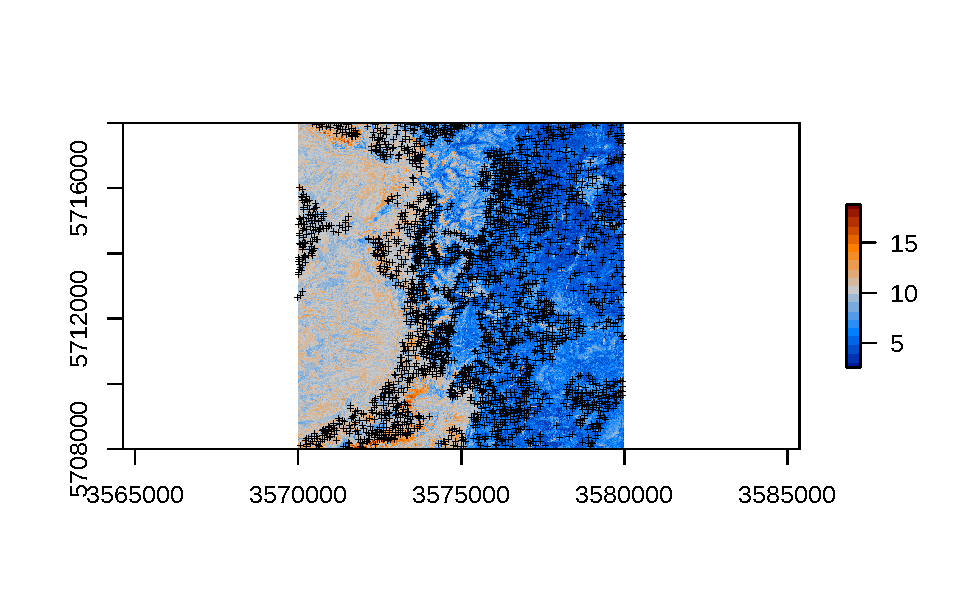
\includegraphics[width=0.9\linewidth]{resampling_files/figure-latex/eberg-var-eml-1} 

}

\caption{Prediction errors for the clay content based on the forestError package and Ensemble ML.}\label{fig:eberg-var-eml}
\end{figure}

In the previous examples we have shown that the actual samples from the Ebergotzen
dataset are actually clustered and cover only agricultural land. Can we
still use these samples to estimate the mapping accuracy for the whole area?
The answer is yes, but we need to be aware that our estimate might be biased
(usually over-optimistic) and we need to do our best to reduce the over-fitting
effects by implementing some of the strategies above e.g.: assign different
weights to training points, and/or implement blocking settings.

Assuming that forest soils are possibly very different from agricultural
soils, once we collect new sampling in the forest part of the study area we
might discovering that the actual mapping accuracy we estimated for the whole
study area using only agricultural soil samples is significantly lower than what
we have estimated in Fig. \ref{fig:eberg-var-eml}.

\begin{figure}

{\centering \includegraphics[width=0.7\linewidth]{./img/Fig_zone_radius_CV} 

}

\caption{Example of effects of the size of the spatial blocking (buffer) on mapping accuracy.}\label{fig:example-cv}
\end{figure}

Fig. \ref{fig:example-cv} shows the usual effect of spatial blocking (for varying buffer size) on the
Cross-Validation accuracy \citep{pohjankukka2017estimating}. Note that the accuracy
tends to stabilize at some distance, although too strict blocking can also lead
to over-pessimistic estimates of accuracy hence bias in predictions \citep[@][]{Wadoux2021EM}.
In the Ebergotzen case, prediction error could be over-pessimistic although the
block size is relatively small considering the size of the study area.
On the other hand, if the training points are clustered, blocking becomes
important because otherwise the estimate of error and choice of model parameters
could get over-optimistic \citep{meyer2018improving, lovelace2019geocomputation}.
If in doubt of whether to produce over-optimistic or over-pessimistic estimates of
uncertainty, it is of course ideal to avoid both, but if necessary consider that
somewhat over-pessimistic estimate of accuracy could be slightly more \emph{on a safe side} \citep{roberts2017cross}.

\hypertarget{testing-mapping-accuracy-using-resampling-and-blocking}{%
\section{Testing mapping accuracy using resampling and blocking}\label{testing-mapping-accuracy-using-resampling-and-blocking}}

We can switch to the Edgeroi dataset \citep{malone2009mapping} that is originally
based on \emph{designed} sampling and as such is more interesting for assessing
effects of various blocking strategies on overall mapping accuracy. We can load
the dataset and prepare a regression matrix by using \citep{hengl2019predictive}:

\begin{Shaded}
\begin{Highlighting}[]
\FunctionTok{data}\NormalTok{(edgeroi)}
\NormalTok{edgeroi.sp }\OtherTok{\textless{}{-}}\NormalTok{ edgeroi}\SpecialCharTok{$}\NormalTok{sites}
\FunctionTok{coordinates}\NormalTok{(edgeroi.sp) }\OtherTok{\textless{}{-}} \ErrorTok{\textasciitilde{}}\NormalTok{ LONGDA94 }\SpecialCharTok{+}\NormalTok{ LATGDA94}
\FunctionTok{proj4string}\NormalTok{(edgeroi.sp) }\OtherTok{\textless{}{-}} \FunctionTok{CRS}\NormalTok{(}\StringTok{"+proj=longlat +ellps=GRS80 +towgs84=0,0,0,0,0,0,0 +no\_defs"}\NormalTok{)}
\NormalTok{edgeroi.sp }\OtherTok{\textless{}{-}} \FunctionTok{spTransform}\NormalTok{(edgeroi.sp, }\FunctionTok{CRS}\NormalTok{(}\StringTok{"+init=epsg:28355"}\NormalTok{))}
\FunctionTok{length}\NormalTok{(edgeroi.sp)}
\CommentTok{\#\textgreater{} [1] 359}
\NormalTok{h2 }\OtherTok{\textless{}{-}} \FunctionTok{hor2xyd}\NormalTok{(edgeroi}\SpecialCharTok{$}\NormalTok{horizons)}
\NormalTok{edgeroi.grids}\FloatTok{.100}\NormalTok{m }\OtherTok{=} \FunctionTok{readRDS}\NormalTok{(}\StringTok{"./extdata/edgeroi.grids.100m.rds"}\NormalTok{)}
\NormalTok{edgeroi.grids }\OtherTok{=}\NormalTok{ landmap}\SpecialCharTok{::}\FunctionTok{spc}\NormalTok{(edgeroi.grids}\FloatTok{.100}\NormalTok{m[}\SpecialCharTok{{-}}\DecValTok{1}\NormalTok{])}
\CommentTok{\#\textgreater{} Converting covariates to principal components...}
\end{Highlighting}
\end{Shaded}

\begin{Shaded}
\begin{Highlighting}[]
\FunctionTok{plot}\NormalTok{(}\FunctionTok{raster}\NormalTok{(edgeroi.grids}\SpecialCharTok{@}\NormalTok{predicted[}\DecValTok{1}\NormalTok{]))}
\FunctionTok{points}\NormalTok{(edgeroi.sp, }\AttributeTok{pch=}\StringTok{"+"}\NormalTok{)}
\end{Highlighting}
\end{Shaded}

\begin{figure}

{\centering 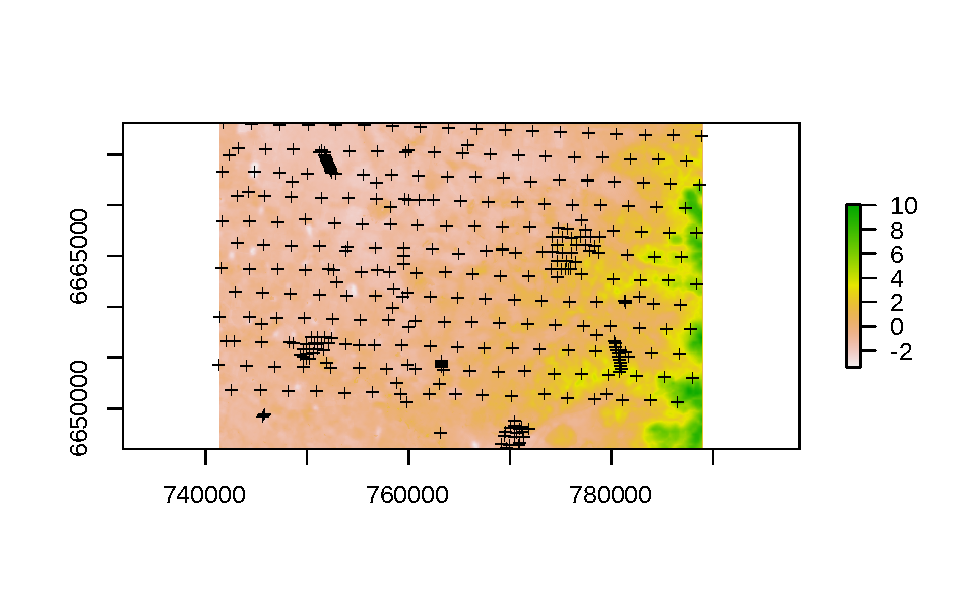
\includegraphics[width=0.9\linewidth]{resampling_files/figure-latex/edgeroi-map-1} 

}

\caption{The Edgeroi dataset consisting of 359 soil profiles.}\label{fig:edgeroi-map}
\end{figure}

The dataset documentation indicates that from a total of 359 profiles, 210 soil profiles
were sampled on a systematic, equilateral triangular grid with a spacing of 2.8 km
between sites; the further 131 soil profiles are distributed more irregularly
or on transects \citep{malone2009mapping}. This is hence a \textbf{hybrid sampling design}
but in general satisfying IID, and hence any subsample of these points should give
an unbiased estimate of the mapping accuracy. We first prepare a regression matrix that includes
all covariates, location IDs and we also add a spatial grid of 500-m size:

\begin{Shaded}
\begin{Highlighting}[]
\NormalTok{grdE }\OtherTok{\textless{}{-}}\NormalTok{ sp}\SpecialCharTok{::}\FunctionTok{GridTopology}\NormalTok{(}\AttributeTok{cellcentre.offset=}\NormalTok{edgeroi.grids}\FloatTok{.100}\NormalTok{m}\SpecialCharTok{@}\NormalTok{bbox[,}\DecValTok{1}\NormalTok{], }\AttributeTok{cellsize=}\FunctionTok{rep}\NormalTok{(}\DecValTok{500}\NormalTok{,}\DecValTok{2}\NormalTok{),}
                        \AttributeTok{cells.dim=}\FunctionTok{c}\NormalTok{(}\FunctionTok{ceiling}\NormalTok{(}\FunctionTok{abs}\NormalTok{(}\FunctionTok{diff}\NormalTok{(edgeroi.grids}\FloatTok{.100}\NormalTok{m}\SpecialCharTok{@}\NormalTok{bbox[}\DecValTok{1}\NormalTok{,])}\SpecialCharTok{/}\DecValTok{500}\NormalTok{))}\SpecialCharTok{+}\DecValTok{1}\NormalTok{,}
                        \FunctionTok{ceiling}\NormalTok{(}\FunctionTok{abs}\NormalTok{(}\FunctionTok{diff}\NormalTok{(edgeroi.grids}\FloatTok{.100}\NormalTok{m}\SpecialCharTok{@}\NormalTok{bbox[}\DecValTok{2}\NormalTok{,])}\SpecialCharTok{/}\DecValTok{500}\NormalTok{))}\SpecialCharTok{+}\DecValTok{1}\NormalTok{))}
\NormalTok{rE.sp }\OtherTok{\textless{}{-}}\NormalTok{ sp}\SpecialCharTok{::}\FunctionTok{SpatialGridDataFrame}\NormalTok{(grdE, }\AttributeTok{proj4string =}\NormalTok{ edgeroi.grids}\FloatTok{.100}\NormalTok{m}\SpecialCharTok{@}\NormalTok{proj4string,}
                    \AttributeTok{data=}\FunctionTok{data.frame}\NormalTok{(}\AttributeTok{gid=}\DecValTok{1}\SpecialCharTok{:}\NormalTok{(grdE}\SpecialCharTok{@}\NormalTok{cells.dim[}\DecValTok{1}\NormalTok{] }\SpecialCharTok{*}\NormalTok{ grdE}\SpecialCharTok{@}\NormalTok{cells.dim[}\DecValTok{2}\NormalTok{])))}
\NormalTok{ovF }\OtherTok{\textless{}{-}}\NormalTok{ sp}\SpecialCharTok{::}\FunctionTok{over}\NormalTok{(edgeroi.sp, edgeroi.grids}\SpecialCharTok{@}\NormalTok{predicted)}
\NormalTok{ovF}\SpecialCharTok{$}\NormalTok{SOURCEID }\OtherTok{\textless{}{-}}\NormalTok{ edgeroi.sp}\SpecialCharTok{$}\NormalTok{SOURCEID}
\NormalTok{ovF}\SpecialCharTok{$}\NormalTok{gid }\OtherTok{\textless{}{-}}\NormalTok{ sp}\SpecialCharTok{::}\FunctionTok{over}\NormalTok{(edgeroi.sp, rE.sp)}\SpecialCharTok{$}\NormalTok{gid}
\NormalTok{ovF}\SpecialCharTok{$}\NormalTok{x }\OtherTok{=}\NormalTok{ edgeroi.sp}\SpecialCharTok{@}\NormalTok{coords[,}\DecValTok{1}\NormalTok{]}
\NormalTok{ovF}\SpecialCharTok{$}\NormalTok{y }\OtherTok{=}\NormalTok{ edgeroi.sp}\SpecialCharTok{@}\NormalTok{coords[,}\DecValTok{2}\NormalTok{]}
\NormalTok{rmF }\OtherTok{\textless{}{-}}\NormalTok{ plyr}\SpecialCharTok{::}\FunctionTok{join\_all}\NormalTok{(}\AttributeTok{dfs =} \FunctionTok{list}\NormalTok{(edgeroi}\SpecialCharTok{$}\NormalTok{sites, h2, ovF))}
\CommentTok{\#\textgreater{} Joining by: SOURCEID}
\CommentTok{\#\textgreater{} Joining by: SOURCEID}
\end{Highlighting}
\end{Shaded}

This produces a regression matrix with unique IDs of profiles \texttt{SOURCEID}, spatial
block IDs (\texttt{gid}) and all target and covariate layers.

We can now fit a model to predict soil organic carbon content (in g/kg) in 3D:

\begin{Shaded}
\begin{Highlighting}[]
\NormalTok{rmF}\SpecialCharTok{$}\NormalTok{log.ORCDRC }\OtherTok{=} \FunctionTok{log1p}\NormalTok{(rmF}\SpecialCharTok{$}\NormalTok{ORCDRC)}
\NormalTok{formulaStringPF }\OtherTok{\textless{}{-}} \FunctionTok{as.formula}\NormalTok{(}\FunctionTok{paste0}\NormalTok{(}\StringTok{"log.ORCDRC \textasciitilde{} DEPTH + "}\NormalTok{, }\FunctionTok{paste0}\NormalTok{(}\StringTok{"PC"}\NormalTok{, }\DecValTok{1}\SpecialCharTok{:}\DecValTok{10}\NormalTok{, }\AttributeTok{collapse =} \StringTok{"+"}\NormalTok{)))}
\NormalTok{rmPF }\OtherTok{\textless{}{-}}\NormalTok{ rmF[}\FunctionTok{complete.cases}\NormalTok{(rmF[,}\FunctionTok{all.vars}\NormalTok{(formulaStringPF)]),]}
\CommentTok{\#str(rmPF[,all.vars(formulaStringPF)])}
\end{Highlighting}
\end{Shaded}

We first fit a model distribution of soil organic carbon ignoring any spatial
clustering, overlap in 3rd dimension (soil depth) or similar:

\begin{Shaded}
\begin{Highlighting}[]
\NormalTok{soc.rf }\OtherTok{=} \FunctionTok{ranger}\NormalTok{(formulaStringPF, rmPF)}
\NormalTok{soc.rf}
\CommentTok{\#\textgreater{} Ranger result}
\CommentTok{\#\textgreater{} }
\CommentTok{\#\textgreater{} Call:}
\CommentTok{\#\textgreater{}  ranger(formulaStringPF, rmPF) }
\CommentTok{\#\textgreater{} }
\CommentTok{\#\textgreater{} Type:                             Regression }
\CommentTok{\#\textgreater{} Number of trees:                  500 }
\CommentTok{\#\textgreater{} Sample size:                      5001 }
\CommentTok{\#\textgreater{} Number of independent variables:  11 }
\CommentTok{\#\textgreater{} Mtry:                             3 }
\CommentTok{\#\textgreater{} Target node size:                 5 }
\CommentTok{\#\textgreater{} Variable importance mode:         none }
\CommentTok{\#\textgreater{} Splitrule:                        variance }
\CommentTok{\#\textgreater{} OOB prediction error (MSE):       0.1116369 }
\CommentTok{\#\textgreater{} R squared (OOB):                  0.8166682}
\end{Highlighting}
\end{Shaded}

If we compare this model with an Ensemble ML where whole blocks i.e.~including
also whole soil profiles are taken out from modeling:

\begin{Shaded}
\begin{Highlighting}[]
\NormalTok{SL.library2 }\OtherTok{=} \FunctionTok{c}\NormalTok{(}\StringTok{"regr.ranger"}\NormalTok{, }\StringTok{"regr.glm"}\NormalTok{, }\StringTok{"regr.cvglmnet"}\NormalTok{, }\StringTok{"regr.xgboost"}\NormalTok{, }\StringTok{"regr.ksvm"}\NormalTok{)}
\NormalTok{lrnsE }\OtherTok{\textless{}{-}} \FunctionTok{lapply}\NormalTok{(SL.library2, mlr}\SpecialCharTok{::}\NormalTok{makeLearner)}
\NormalTok{tskE }\OtherTok{\textless{}{-}}\NormalTok{ mlr}\SpecialCharTok{::}\FunctionTok{makeRegrTask}\NormalTok{(}\AttributeTok{data =}\NormalTok{ rmPF[,}\FunctionTok{all.vars}\NormalTok{(formulaStringPF)], }\AttributeTok{target=}\StringTok{"log.ORCDRC"}\NormalTok{, }
                          \AttributeTok{blocking =} \FunctionTok{as.factor}\NormalTok{(rmPF}\SpecialCharTok{$}\NormalTok{gid))}
\NormalTok{initE.m }\OtherTok{\textless{}{-}}\NormalTok{ mlr}\SpecialCharTok{::}\FunctionTok{makeStackedLearner}\NormalTok{(lrnsE, }\AttributeTok{method =} \StringTok{"stack.cv"}\NormalTok{, }
                  \AttributeTok{super.learner =} \StringTok{"regr.lm"}\NormalTok{,}
                  \AttributeTok{resampling=}\NormalTok{mlr}\SpecialCharTok{::}\FunctionTok{makeResampleDesc}\NormalTok{(}\AttributeTok{method =} \StringTok{"CV"}\NormalTok{, }\AttributeTok{blocking.cv=}\ConstantTok{TRUE}\NormalTok{))}
\NormalTok{emlE }\OtherTok{=} \FunctionTok{train}\NormalTok{(initE.m, tskE)}
\CommentTok{\#\textgreater{} Exporting objects to slaves for mode socket: .mlr.slave.options}
\CommentTok{\#\textgreater{} Mapping in parallel: mode = socket; level = mlr.resample; cpus = 32; elements = 10.}
\CommentTok{\#\textgreater{} Exporting objects to slaves for mode socket: .mlr.slave.options}
\CommentTok{\#\textgreater{} Mapping in parallel: mode = socket; level = mlr.resample; cpus = 32; elements = 10.}
\CommentTok{\#\textgreater{} Exporting objects to slaves for mode socket: .mlr.slave.options}
\CommentTok{\#\textgreater{} Mapping in parallel: mode = socket; level = mlr.resample; cpus = 32; elements = 10.}
\CommentTok{\#\textgreater{} Exporting objects to slaves for mode socket: .mlr.slave.options}
\CommentTok{\#\textgreater{} Mapping in parallel: mode = socket; level = mlr.resample; cpus = 32; elements = 10.}
\CommentTok{\#\textgreater{} [12:18:24] }\AlertTok{WARNING}\CommentTok{: amalgamation/../src/objective/regression\_obj.cu:170: reg:linear is now deprecated in favor of reg:squarederror.}
\CommentTok{\#\textgreater{} Exporting objects to slaves for mode socket: .mlr.slave.options}
\CommentTok{\#\textgreater{} Mapping in parallel: mode = socket; level = mlr.resample; cpus = 32; elements = 10.}
\FunctionTok{summary}\NormalTok{(emlE}\SpecialCharTok{$}\NormalTok{learner.model}\SpecialCharTok{$}\NormalTok{super.model}\SpecialCharTok{$}\NormalTok{learner.model)}
\CommentTok{\#\textgreater{} }
\CommentTok{\#\textgreater{} Call:}
\CommentTok{\#\textgreater{} stats::lm(formula = f, data = d)}
\CommentTok{\#\textgreater{} }
\CommentTok{\#\textgreater{} Residuals:}
\CommentTok{\#\textgreater{}     Min      1Q  Median      3Q     Max }
\CommentTok{\#\textgreater{} {-}2.1642 {-}0.2550 {-}0.0232  0.2376  3.1830 }
\CommentTok{\#\textgreater{} }
\CommentTok{\#\textgreater{} Coefficients:}
\CommentTok{\#\textgreater{}               Estimate Std. Error t value Pr(\textgreater{}|t|)    }
\CommentTok{\#\textgreater{} (Intercept)   {-}0.17386    0.03557  {-}4.887 1.05e{-}06 ***}
\CommentTok{\#\textgreater{} regr.ranger    0.83042    0.04432  18.736  \textless{} 2e{-}16 ***}
\CommentTok{\#\textgreater{} regr.glm       0.42906    0.07066   6.072 1.36e{-}09 ***}
\CommentTok{\#\textgreater{} regr.cvglmnet {-}0.37021    0.07626  {-}4.855 1.24e{-}06 ***}
\CommentTok{\#\textgreater{} regr.xgboost   0.20284    0.09370   2.165   0.0305 *  }
\CommentTok{\#\textgreater{} regr.ksvm      0.12077    0.02840   4.253 2.15e{-}05 ***}
\CommentTok{\#\textgreater{} {-}{-}{-}}
\CommentTok{\#\textgreater{} Signif. codes:  0 \textquotesingle{}***\textquotesingle{} 0.001 \textquotesingle{}**\textquotesingle{} 0.01 \textquotesingle{}*\textquotesingle{} 0.05 \textquotesingle{}.\textquotesingle{} 0.1 \textquotesingle{} \textquotesingle{} 1}
\CommentTok{\#\textgreater{} }
\CommentTok{\#\textgreater{} Residual standard error: 0.449 on 4995 degrees of freedom}
\CommentTok{\#\textgreater{} Multiple R{-}squared:  0.6693, Adjusted R{-}squared:  0.6689 }
\CommentTok{\#\textgreater{} F{-}statistic:  2022 on 5 and 4995 DF,  p{-}value: \textless{} 2.2e{-}16}
\end{Highlighting}
\end{Shaded}

Notice a large difference in the model accuracy with R-square dropping from
about 0.82 to 0.65. How can we check which of the two models is more accurate /
which shows a more realistic mapping accuracy? We can again generate pseudo-grid
samples e.g.~10 subsets where in each subset we make sure that the points are at
least 3.5-km apart and are taken selected randomly:

\begin{Shaded}
\begin{Highlighting}[]
\NormalTok{subE.lst }\OtherTok{=} \FunctionTok{lapply}\NormalTok{(}\DecValTok{1}\SpecialCharTok{:}\DecValTok{10}\NormalTok{, }\ControlFlowTok{function}\NormalTok{(i)\{landmap}\SpecialCharTok{::}\FunctionTok{sample.grid}\NormalTok{(edgeroi.sp, }\FunctionTok{c}\NormalTok{(}\FloatTok{3.5e3}\NormalTok{, }\FloatTok{3.5e3}\NormalTok{), }\AttributeTok{n=}\DecValTok{1}\NormalTok{)\})}
\end{Highlighting}
\end{Shaded}

\begin{Shaded}
\begin{Highlighting}[]
\NormalTok{lE1 }\OtherTok{\textless{}{-}} \FunctionTok{list}\NormalTok{(}\StringTok{"sp.points"}\NormalTok{, subE.lst[[}\DecValTok{1}\NormalTok{]]}\SpecialCharTok{$}\NormalTok{subset, }\AttributeTok{pch=}\StringTok{"+"}\NormalTok{, }\AttributeTok{col=}\StringTok{"black"}\NormalTok{)}
\FunctionTok{spplot}\NormalTok{(subE.lst[[}\DecValTok{1}\NormalTok{]]}\SpecialCharTok{$}\NormalTok{grid, }\AttributeTok{scales=}\FunctionTok{list}\NormalTok{(}\AttributeTok{draw=}\ConstantTok{TRUE}\NormalTok{),}
   \AttributeTok{col.regions=}\StringTok{"grey"}\NormalTok{, }\AttributeTok{sp.layout=}\FunctionTok{list}\NormalTok{(lE1), }\AttributeTok{colorkey=}\ConstantTok{FALSE}\NormalTok{)}
\end{Highlighting}
\end{Shaded}

\begin{figure}

{\centering 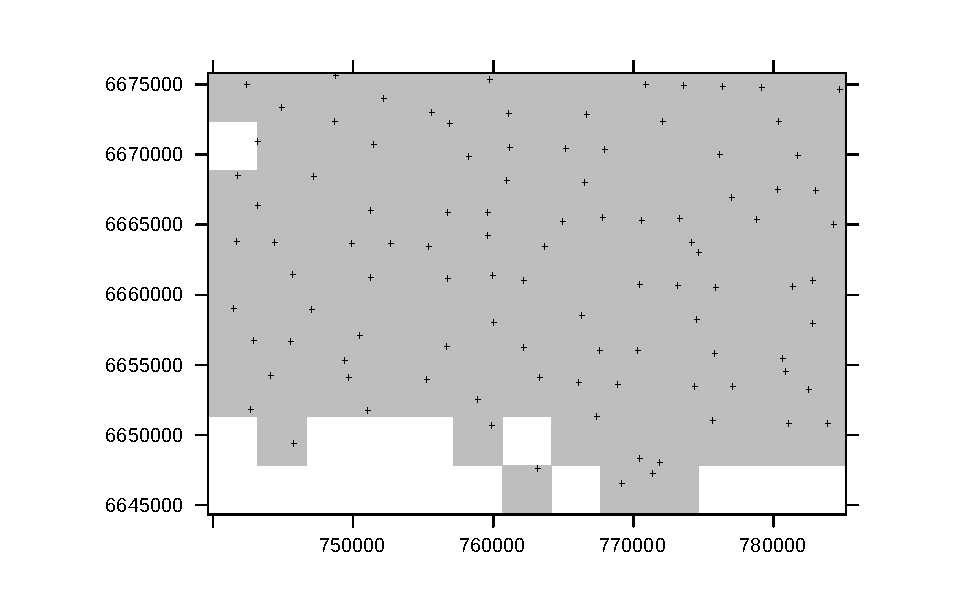
\includegraphics[width=0.9\linewidth]{resampling_files/figure-latex/edgeroi-grid-sample-1} 

}

\caption{Resampling original points using `sample.grid` function for the Edgeroi dataset.}\label{fig:edgeroi-grid-sample}
\end{figure}

So in any random pseudo-grid subset we take out about 100 profiles from 359 and
keep for validation only. We can next repeatedly fit models using the two
approaches and derive prediction errors. First, for simple model ignoring any
spatial clustering / soil profile locations:

\begin{Shaded}
\begin{Highlighting}[]
\NormalTok{rf.soc.lst }\OtherTok{=} \FunctionTok{lapply}\NormalTok{(}\DecValTok{1}\SpecialCharTok{:}\FunctionTok{length}\NormalTok{(subE.lst), }\ControlFlowTok{function}\NormalTok{(i)\{}
\NormalTok{        sel }\OtherTok{\textless{}{-}} \SpecialCharTok{!}\NormalTok{rmPF}\SpecialCharTok{$}\NormalTok{SOURCEID }\SpecialCharTok{\%in\%}\NormalTok{ subE.lst[[i]]}\SpecialCharTok{$}\NormalTok{subset}\SpecialCharTok{$}\NormalTok{SOURCEID;}
\NormalTok{        y }\OtherTok{\textless{}{-}}\NormalTok{ ranger}\SpecialCharTok{::}\FunctionTok{ranger}\NormalTok{(formulaStringPF, rmPF[sel,]);}
\NormalTok{        out }\OtherTok{\textless{}{-}} \FunctionTok{data.frame}\NormalTok{(}\AttributeTok{meas=}\NormalTok{rmPF[}\SpecialCharTok{!}\NormalTok{sel,}\StringTok{"log.ORCDRC"}\NormalTok{], }\AttributeTok{pred=}\FunctionTok{predict}\NormalTok{(y, rmPF[}\SpecialCharTok{!}\NormalTok{sel,])}\SpecialCharTok{$}\NormalTok{predictions);}
        \FunctionTok{return}\NormalTok{(out)}
\NormalTok{      \}}
\NormalTok{)}
\NormalTok{rf.cv }\OtherTok{=} \FunctionTok{do.call}\NormalTok{(rbind, rf.soc.lst)}
\NormalTok{Metrics}\SpecialCharTok{::}\FunctionTok{rmse}\NormalTok{(rf.cv}\SpecialCharTok{$}\NormalTok{meas, rf.cv}\SpecialCharTok{$}\NormalTok{pred)}
\CommentTok{\#\textgreater{} [1] 0.4343792}
\end{Highlighting}
\end{Shaded}

This gives an RMSPE of 0.44, which is higher than what is reported by the OOB for RF
without blocking. The accuracy plot shows that the \href{https://rdrr.io/cran/yardstick/man/ccc.html}{Concordance Correlation Coefficient (CCC)}
is about 0.79 (corresponding to a R-square of about 0.62 and thus significantly
less than what is reported by ranger):

\begin{Shaded}
\begin{Highlighting}[]
\NormalTok{t.b }\OtherTok{=} \FunctionTok{quantile}\NormalTok{(}\FunctionTok{log1p}\NormalTok{(rmPF}\SpecialCharTok{$}\NormalTok{ORCDRC), }\FunctionTok{c}\NormalTok{(}\FloatTok{0.001}\NormalTok{, }\FloatTok{0.01}\NormalTok{, }\FloatTok{0.999}\NormalTok{), }\AttributeTok{na.rm=}\ConstantTok{TRUE}\NormalTok{)}
\FunctionTok{plot\_hexbin}\NormalTok{(}\AttributeTok{varn=}\StringTok{"SOC\_RF"}\NormalTok{, }\AttributeTok{breaks=}\FunctionTok{c}\NormalTok{(t.b[}\DecValTok{1}\NormalTok{], }\FunctionTok{seq}\NormalTok{(t.b[}\DecValTok{2}\NormalTok{], t.b[}\DecValTok{3}\NormalTok{], }\AttributeTok{length=}\DecValTok{25}\NormalTok{)), }
      \AttributeTok{meas=}\NormalTok{rf.cv}\SpecialCharTok{$}\NormalTok{meas, }\AttributeTok{pred=}\NormalTok{rf.cv}\SpecialCharTok{$}\NormalTok{pred, }\AttributeTok{main=}\StringTok{"SOC [RF]"}\NormalTok{)}
\end{Highlighting}
\end{Shaded}

\begin{figure}

{\centering \includegraphics[width=0.7\linewidth]{./img/plot_CV_SOC_RF} 

}

\caption{Accuracy plot for soil organic carbon fitted using RF.}\label{fig:ac-soc1}
\end{figure}

We repeat the same process of re-fitting the model using Ensemble ML with spatial
blocking:

\begin{Shaded}
\begin{Highlighting}[]
\NormalTok{eml.soc.lst }\OtherTok{=} \FunctionTok{lapply}\NormalTok{(}\DecValTok{1}\SpecialCharTok{:}\FunctionTok{length}\NormalTok{(subE.lst), }\ControlFlowTok{function}\NormalTok{(i)\{}
\NormalTok{        sel }\OtherTok{\textless{}{-}} \SpecialCharTok{!}\NormalTok{rmPF}\SpecialCharTok{$}\NormalTok{SOURCEID }\SpecialCharTok{\%in\%}\NormalTok{ subE.lst[[i]]}\SpecialCharTok{$}\NormalTok{subset}\SpecialCharTok{$}\NormalTok{SOURCEID;}
\NormalTok{        x }\OtherTok{\textless{}{-}}\NormalTok{ mlr}\SpecialCharTok{::}\FunctionTok{makeRegrTask}\NormalTok{(}\AttributeTok{data =}\NormalTok{ rmPF[sel,}\FunctionTok{all.vars}\NormalTok{(formulaStringPF)], }
                  \AttributeTok{target=}\StringTok{"log.ORCDRC"}\NormalTok{, }\AttributeTok{blocking =} \FunctionTok{as.factor}\NormalTok{(rmPF}\SpecialCharTok{$}\NormalTok{gid[sel]));}
\NormalTok{        y }\OtherTok{\textless{}{-}} \FunctionTok{train}\NormalTok{(initE.m, x)}
\NormalTok{        out }\OtherTok{\textless{}{-}} \FunctionTok{data.frame}\NormalTok{(}\AttributeTok{meas=}\NormalTok{rmPF[}\SpecialCharTok{!}\NormalTok{sel,}\StringTok{"log.ORCDRC"}\NormalTok{], }\AttributeTok{pred=}\FunctionTok{predict}\NormalTok{(y, }\AttributeTok{newdata=}\NormalTok{rmPF[}\SpecialCharTok{!}\NormalTok{sel, y}\SpecialCharTok{$}\NormalTok{features])}\SpecialCharTok{$}\NormalTok{data}\SpecialCharTok{$}\NormalTok{response);}
        \FunctionTok{return}\NormalTok{(out)}
\NormalTok{      \}}
\NormalTok{)}
\NormalTok{eml.cv }\OtherTok{=} \FunctionTok{do.call}\NormalTok{(rbind, eml.soc.lst)}
\NormalTok{Metrics}\SpecialCharTok{::}\FunctionTok{rmse}\NormalTok{(eml.cv}\SpecialCharTok{$}\NormalTok{meas, eml.cv}\SpecialCharTok{$}\NormalTok{pred)}
\end{Highlighting}
\end{Shaded}

\begin{Shaded}
\begin{Highlighting}[]
\FunctionTok{plot\_hexbin}\NormalTok{(}\AttributeTok{varn=}\StringTok{"SOC\_EML"}\NormalTok{, }\AttributeTok{breaks=}\FunctionTok{c}\NormalTok{(t.b[}\DecValTok{1}\NormalTok{], }\FunctionTok{seq}\NormalTok{(t.b[}\DecValTok{2}\NormalTok{], t.b[}\DecValTok{3}\NormalTok{], }\AttributeTok{length=}\DecValTok{25}\NormalTok{)), }
      \AttributeTok{meas=}\NormalTok{eml.cv}\SpecialCharTok{$}\NormalTok{meas, }\AttributeTok{pred=}\NormalTok{eml.cv}\SpecialCharTok{$}\NormalTok{pred, }\AttributeTok{main=}\StringTok{"SOC [EML]"}\NormalTok{)}
\end{Highlighting}
\end{Shaded}

\begin{figure}

{\centering \includegraphics[width=0.7\linewidth]{./img/plot_CV_SOC_EML} 

}

\caption{Accuracy plot for soil organic carbon fitted using Ensemble Machine Learning with spatial blocking.}\label{fig:ac-soc2}
\end{figure}

So in summary, independent validation using pseudo-probability samples indicates
that the Ensemble ML produces more accurate predictions (in this case only slightly
better) and the RMSE estimated by the meta-learner the Ensemble ML approach is more
realistic (\texttt{Residual\ standard\ error:\ 0.45}). This clearly demonstrates that spatial
blocking is important to (a) prevent from over-fitting, (b) produce a more realistic
estimate of the uncertainty / mapping accuracy. Ensemble ML comes at costs of
at the order of magnitude higher computing costs however.

We can again plot the predictions produced by two methods next to each other:

\begin{Shaded}
\begin{Highlighting}[]
\NormalTok{newdata }\OtherTok{=}\NormalTok{ edgeroi.grids}\SpecialCharTok{@}\NormalTok{predicted}\SpecialCharTok{@}\NormalTok{data[,}\FunctionTok{paste0}\NormalTok{(}\StringTok{"PC"}\NormalTok{, }\DecValTok{1}\SpecialCharTok{:}\DecValTok{10}\NormalTok{)]}
\NormalTok{newdata}\SpecialCharTok{$}\NormalTok{DEPTH }\OtherTok{=} \DecValTok{5}
\end{Highlighting}
\end{Shaded}

\begin{Shaded}
\begin{Highlighting}[]
\NormalTok{edgeroi.grids}\FloatTok{.100}\NormalTok{m}\SpecialCharTok{$}\NormalTok{rf\_soc\_5cm }\OtherTok{=} \FunctionTok{predict}\NormalTok{(soc.rf, newdata)}\SpecialCharTok{$}\NormalTok{predictions}
\NormalTok{edgeroi.grids}\FloatTok{.100}\NormalTok{m}\SpecialCharTok{$}\NormalTok{eml\_soc\_5cm }\OtherTok{=} \FunctionTok{predict}\NormalTok{(emlE, }\AttributeTok{newdata=}\NormalTok{newdata[,emlE}\SpecialCharTok{$}\NormalTok{features])}\SpecialCharTok{$}\NormalTok{data}\SpecialCharTok{$}\NormalTok{response}
\NormalTok{l.pnts }\OtherTok{\textless{}{-}} \FunctionTok{list}\NormalTok{(}\StringTok{"sp.points"}\NormalTok{, edgeroi.sp, }\AttributeTok{pch=}\StringTok{"+"}\NormalTok{, }\AttributeTok{col=}\StringTok{"black"}\NormalTok{)}
\FunctionTok{spplot}\NormalTok{(edgeroi.grids}\FloatTok{.100}\NormalTok{m[}\FunctionTok{c}\NormalTok{(}\StringTok{"rf\_soc\_5cm"}\NormalTok{, }\StringTok{"eml\_soc\_5cm"}\NormalTok{)], }
       \AttributeTok{sp.layout =} \FunctionTok{list}\NormalTok{(l.pnts), }\AttributeTok{col.regions=}\NormalTok{SAGA\_pal[[}\DecValTok{1}\NormalTok{]])}
\end{Highlighting}
\end{Shaded}

\begin{figure}

{\centering \includegraphics[width=1\linewidth]{./img/edgeroi_predictions_SOC_5cm} 

}

\caption{Predictions of soil organic carbon (in log-scale) based on Random Forest (RF) and Ensemble ML (EML).}\label{fig:pred-soc}
\end{figure}

Which shows that the Ensemble ML seems to predict significantly higher SOC in the
hillands (right part of the study area), so again significant difference in predictions
between the two models. Even though the Ensemble ML with spatial blocking is only
slightly better in accuracy (RMSE based on 10-times out-of-bag declustered validation points),
these results confirm that it helps produce a more realistic map of RMSPE.
This matches the result of \citet{roberts2017cross} and \citet{meyer2018improving} who suggest that block cross-validation is
nearly universally more appropriate than random cross-validation if the goal is
predicting to new data or predictor space, or for selecting causal predictors.

We can also map the prediction errors:

\begin{Shaded}
\begin{Highlighting}[]
\NormalTok{emlE.t }\OtherTok{=}\NormalTok{ emlE}\SpecialCharTok{$}\NormalTok{learner.model}\SpecialCharTok{$}\NormalTok{super.model}\SpecialCharTok{$}\NormalTok{learner.model}\SpecialCharTok{$}\NormalTok{terms}
\FunctionTok{paste}\NormalTok{(emlE.t)}
\CommentTok{\#\textgreater{} [1] "\textasciitilde{}"                                                                }
\CommentTok{\#\textgreater{} [2] "log.ORCDRC"                                                       }
\CommentTok{\#\textgreater{} [3] "regr.ranger + regr.glm + regr.cvglmnet + regr.xgboost + regr.ksvm"}
\NormalTok{emlE.m }\OtherTok{=}\NormalTok{ emlE}\SpecialCharTok{$}\NormalTok{learner.model}\SpecialCharTok{$}\NormalTok{super.model}\SpecialCharTok{$}\NormalTok{learner.model}\SpecialCharTok{$}\NormalTok{model}
\NormalTok{emlE.qr }\OtherTok{\textless{}{-}}\NormalTok{ ranger}\SpecialCharTok{::}\FunctionTok{ranger}\NormalTok{(emlE.t, emlE.m, }\AttributeTok{num.trees=}\DecValTok{85}\NormalTok{, }\AttributeTok{importance=}\StringTok{"impurity"}\NormalTok{, }
                         \AttributeTok{quantreg=}\ConstantTok{TRUE}\NormalTok{, }\AttributeTok{keep.inbag =} \ConstantTok{TRUE}\NormalTok{)}
\NormalTok{outE.c }\OtherTok{\textless{}{-}} \FunctionTok{as.data.frame}\NormalTok{(mlr}\SpecialCharTok{::}\FunctionTok{getStackedBaseLearnerPredictions}\NormalTok{(emlE, }
                                      \AttributeTok{newdata=}\NormalTok{newdata[,emlE}\SpecialCharTok{$}\NormalTok{features]))}
\NormalTok{predE.q }\OtherTok{=}\NormalTok{ forestError}\SpecialCharTok{::}\FunctionTok{quantForestError}\NormalTok{(emlE.qr, }
                    \AttributeTok{X.train =}\NormalTok{ emlE.m[,}\FunctionTok{all.vars}\NormalTok{(emlE.t)[}\SpecialCharTok{{-}}\DecValTok{1}\NormalTok{]], }
                    \AttributeTok{X.test =}\NormalTok{ outE.c, }
                    \AttributeTok{Y.train =}\NormalTok{ emlE.m[,}\FunctionTok{all.vars}\NormalTok{(emlE.t)[}\DecValTok{1}\NormalTok{]], }
                    \AttributeTok{alpha =}\NormalTok{ (}\DecValTok{1}\SpecialCharTok{{-}}\NormalTok{(quantiles[}\DecValTok{2}\NormalTok{]}\SpecialCharTok{{-}}\NormalTok{quantiles[}\DecValTok{1}\NormalTok{])), }\AttributeTok{n.cores=}\NormalTok{n.cores)}
\end{Highlighting}
\end{Shaded}

Which again shows where could be the main extrapolation problems i.e.~where
multiple base learners perform poorly:

\begin{Shaded}
\begin{Highlighting}[]
\NormalTok{edgeroi.grids}\FloatTok{.100}\NormalTok{m}\SpecialCharTok{$}\NormalTok{rmspe.soc.eml }\OtherTok{=} \FunctionTok{sqrt}\NormalTok{(predE.q}\SpecialCharTok{$}\NormalTok{estimates}\SpecialCharTok{$}\NormalTok{mspe)}
\FunctionTok{plot}\NormalTok{(}\FunctionTok{raster}\NormalTok{(edgeroi.grids}\FloatTok{.100}\NormalTok{m[}\FunctionTok{c}\NormalTok{(}\StringTok{"rmspe.soc.eml"}\NormalTok{)]), }\AttributeTok{col=}\NormalTok{SAGA\_pal[[}\DecValTok{16}\NormalTok{]])}
\FunctionTok{points}\NormalTok{(edgeroi.sp, }\AttributeTok{pch=}\StringTok{"+"}\NormalTok{, }\AttributeTok{cex=}\NormalTok{.}\DecValTok{8}\NormalTok{)}
\end{Highlighting}
\end{Shaded}

\begin{figure}

{\centering 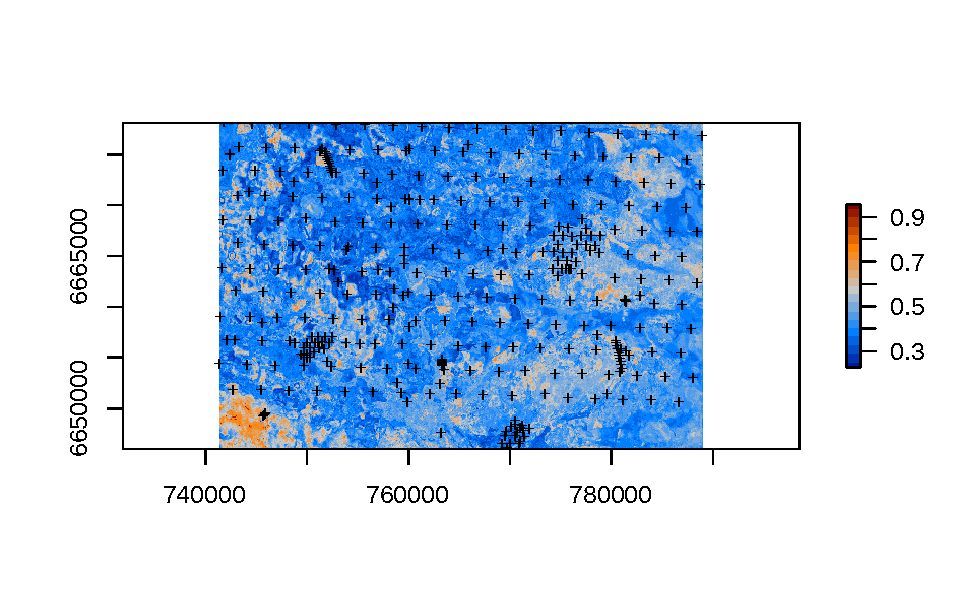
\includegraphics[width=0.9\linewidth]{resampling_files/figure-latex/edgeroi-var-eml-1} 

}

\caption{Prediction errors for the soil organic carbon content based on the forestError package and Ensemble ML.}\label{fig:edgeroi-var-eml}
\end{figure}

\begin{Shaded}
\begin{Highlighting}[]
\NormalTok{rgdal}\SpecialCharTok{::}\FunctionTok{writeGDAL}\NormalTok{(edgeroi.grids}\FloatTok{.100}\NormalTok{m[}\FunctionTok{c}\NormalTok{(}\StringTok{"rmspe.soc.eml"}\NormalTok{)], }
                 \StringTok{"./output/edgeroi\_soc\_rmspe.tif"}\NormalTok{, }
                 \AttributeTok{options=}\FunctionTok{c}\NormalTok{(}\StringTok{"COMPRESS=DEFLATE"}\NormalTok{))}
\end{Highlighting}
\end{Shaded}

The overall mapping accuracy for Edgeroi based on the mean prediction error is thus:

\begin{Shaded}
\begin{Highlighting}[]
\FunctionTok{mean}\NormalTok{(}\FunctionTok{sqrt}\NormalTok{(predE.q}\SpecialCharTok{$}\NormalTok{estimates}\SpecialCharTok{$}\NormalTok{mspe), }\AttributeTok{na.rm=}\ConstantTok{TRUE}\NormalTok{)}
\CommentTok{\#\textgreater{} [1] 0.4352432}
\end{Highlighting}
\end{Shaded}

which in general matches what we get through repeated validation using pseudo-SRS
subsampling.

From this experiment we can conclude that the mapping accuracy estimated using
ranger and out-of-bag samples and ignoring locations of profiles was
probably over-optimistic and hence ranger has possibly over-fitted the target variable.
This is in fact common problem observed with many 3D predictive soil mapping models
where soil profiles basically have ALL the same values of covariates and Random
Forest thus easier predicts values due to overlap in covariate data. For a
discussion on why is important to run internal training and Cross-Validation
using spatial blocking refer also to \citet{gasch2015spatio} and \citet{meyer2018improving}.

\begin{Shaded}
\begin{Highlighting}[]
\NormalTok{parallelMap}\SpecialCharTok{::}\FunctionTok{parallelStop}\NormalTok{()}
\CommentTok{\#\textgreater{} Stopped parallelization. All cleaned up.}
\end{Highlighting}
\end{Shaded}

\hypertarget{resampling-for-spatiotemporal-machine-learning}{%
\chapter{Resampling for spatiotemporal Machine Learning}\label{resampling-for-spatiotemporal-machine-learning}}

You are reading the work-in-progress Spatial Sampling and Resampling for Machine Learning. This chapter is currently draft version, a peer-review publication is pending. You can find the polished first edition at \url{https://opengeohub.github.io/spatial-sampling-ml/}.

\hypertarget{case-study-cookfarm-dataset}{%
\section{Case study: Cookfarm dataset}\label{case-study-cookfarm-dataset}}

We next look at the \href{https://rdrr.io/cran/landmap/man/cookfarm.html}{Cookfarm dataset}, which is available via the landmap
package and described in detail in \citet{gasch2015spatio}:

\begin{Shaded}
\begin{Highlighting}[]
\FunctionTok{library}\NormalTok{(landmap)}
\CommentTok{\#?landmap::cookfarm}
\FunctionTok{data}\NormalTok{(}\StringTok{"cookfarm"}\NormalTok{)}
\end{Highlighting}
\end{Shaded}

This dataset contains spatio-temporal (3D+T) measurements of three soil
properties and a number of spatial and temporal regression covariates.
In this example multiple covariates are used to fit a spatiotemporal model to
predict soil moisture, soil temperature and electrical conductivity in 3D+T
(hence 2 extra dimension beyond spatial dimensions i.e.~a 2D model).

We can load the prediction locations and regression-matrix from:

\begin{Shaded}
\begin{Highlighting}[]
\FunctionTok{library}\NormalTok{(rgdal)}
\FunctionTok{library}\NormalTok{(ranger)}
\NormalTok{cookfarm.rm }\OtherTok{=} \FunctionTok{readRDS}\NormalTok{(}\StringTok{\textquotesingle{}extdata/cookfarm\_st.rds\textquotesingle{}}\NormalTok{)}
\NormalTok{cookfarm.grid }\OtherTok{=} \FunctionTok{readRDS}\NormalTok{(}\StringTok{\textquotesingle{}extdata/cookfarm\_grid10m.rds\textquotesingle{}}\NormalTok{)}
\end{Highlighting}
\end{Shaded}

We are specifically interested in modeling soil moisture (\texttt{VW}) as a function of soil
depth (\texttt{altitude}), elevation (\texttt{DEM}), Topographic Wetness Index
(\texttt{TWI}), Normalized Difference Red Edge Index (\texttt{NDRE.M}), Normalized
Difference Red Edge Index (\texttt{NDRE.sd}), Cumulative precipitation in mm
(\texttt{Precip\_cum}), Maximum measured temperature (\texttt{MaxT\_wrcc}), Minimum
measured temperature (\texttt{MinT\_wrcc}) and the transformed cumulative day
(\texttt{cdayt}):

\begin{Shaded}
\begin{Highlighting}[]
\NormalTok{fm }\OtherTok{\textless{}{-}}\NormalTok{ VW }\SpecialCharTok{\textasciitilde{}}\NormalTok{ altitude}\SpecialCharTok{+}\NormalTok{DEM}\SpecialCharTok{+}\NormalTok{TWI}\SpecialCharTok{+}\NormalTok{NDRE.M}\SpecialCharTok{+}\NormalTok{NDRE.Sd}\SpecialCharTok{+}\NormalTok{Precip\_cum}\SpecialCharTok{+}\NormalTok{MaxT\_wrcc}\SpecialCharTok{+}\NormalTok{MinT\_wrcc}\SpecialCharTok{+}\NormalTok{cdayt}
\end{Highlighting}
\end{Shaded}

We can use the ranger package to fit a random forest model:

\begin{Shaded}
\begin{Highlighting}[]
\NormalTok{m.vw }\OtherTok{=} \FunctionTok{ranger}\NormalTok{(fm, cookfarm.rm, }\AttributeTok{num.trees =} \DecValTok{100}\NormalTok{)}
\NormalTok{m.vw}
\CommentTok{\#\textgreater{} Ranger result}
\CommentTok{\#\textgreater{} }
\CommentTok{\#\textgreater{} Call:}
\CommentTok{\#\textgreater{}  ranger(fm, cookfarm.rm, num.trees = 100) }
\CommentTok{\#\textgreater{} }
\CommentTok{\#\textgreater{} Type:                             Regression }
\CommentTok{\#\textgreater{} Number of trees:                  100 }
\CommentTok{\#\textgreater{} Sample size:                      107851 }
\CommentTok{\#\textgreater{} Number of independent variables:  9 }
\CommentTok{\#\textgreater{} Mtry:                             3 }
\CommentTok{\#\textgreater{} Target node size:                 5 }
\CommentTok{\#\textgreater{} Variable importance mode:         none }
\CommentTok{\#\textgreater{} Splitrule:                        variance }
\CommentTok{\#\textgreater{} OOB prediction error (MSE):       0.0009826038 }
\CommentTok{\#\textgreater{} R squared (OOB):                  0.8479968}
\end{Highlighting}
\end{Shaded}

which shows that a significant model can be fitting using this data with
R-square about 0.85. The accuracy plot shows that the \href{https://rdrr.io/cran/yardstick/man/ccc.html}{Concordance Correlation Coefficient (CCC)}
is high:

\begin{Shaded}
\begin{Highlighting}[]
\NormalTok{vw.b }\OtherTok{=} \FunctionTok{quantile}\NormalTok{(cookfarm.rm}\SpecialCharTok{$}\NormalTok{VW, }\FunctionTok{c}\NormalTok{(}\FloatTok{0.001}\NormalTok{, }\FloatTok{0.01}\NormalTok{, }\FloatTok{0.999}\NormalTok{), }\AttributeTok{na.rm=}\ConstantTok{TRUE}\NormalTok{)}
\FunctionTok{plot\_hexbin}\NormalTok{(}\AttributeTok{varn=}\StringTok{"VW\_RF"}\NormalTok{, }\AttributeTok{breaks=}\FunctionTok{c}\NormalTok{(vw.b[}\DecValTok{1}\NormalTok{], }\FunctionTok{seq}\NormalTok{(vw.b[}\DecValTok{2}\NormalTok{], vw.b[}\DecValTok{3}\NormalTok{], }\AttributeTok{length=}\DecValTok{25}\NormalTok{)), }
      \AttributeTok{meas=}\NormalTok{cookfarm.rm}\SpecialCharTok{$}\NormalTok{VW, }\AttributeTok{pred=}\NormalTok{m.vw}\SpecialCharTok{$}\NormalTok{predictions, }\AttributeTok{main=}\StringTok{"VW [RF]"}\NormalTok{)}
\end{Highlighting}
\end{Shaded}

\begin{figure}

{\centering \includegraphics[width=0.7\linewidth]{./img/plot_CV_VW_RF} 

}

\caption{Accuracy plot for soil moisture content fitted using RF.}\label{fig:ac-vw1}
\end{figure}

This model, however, as shown in \citet{gasch2015spatio}, ignores the fact that many
\texttt{VW} measurements have exactly the same location (monitoring station with four
depths), hence ranger over-fits data and gives unrealistic R-square.
We can instead fit an Ensemble ML model, but we will also use a \textbf{blocking
parameter} that should protect from over-fitting: the unique code of
the station (\texttt{SOURCEID}). This means that \textbf{complete stations} will be
either used for training or for validation. This satisfies the
requirement of \citet{roberts2017cross} for predicting to new data or predictor
space by blocking clustered or overlapping measurements.

We use the same procedure in \texttt{mlr} as in the previous example:

\begin{Shaded}
\begin{Highlighting}[]
\FunctionTok{library}\NormalTok{(mlr)}
\NormalTok{SL.lst }\OtherTok{=} \FunctionTok{c}\NormalTok{(}\StringTok{"regr.ranger"}\NormalTok{, }\StringTok{"regr.gamboost"}\NormalTok{, }\StringTok{"regr.cvglmnet"}\NormalTok{)}
\NormalTok{lrns.st }\OtherTok{\textless{}{-}} \FunctionTok{lapply}\NormalTok{(SL.lst, mlr}\SpecialCharTok{::}\NormalTok{makeLearner)}
\DocumentationTok{\#\# subset to 5\% to speed up computing}
\NormalTok{subs }\OtherTok{\textless{}{-}} \FunctionTok{runif}\NormalTok{(}\FunctionTok{nrow}\NormalTok{(cookfarm.rm))}\SpecialCharTok{\textless{}}\NormalTok{.}\DecValTok{05}
\NormalTok{tsk.st }\OtherTok{\textless{}{-}}\NormalTok{ mlr}\SpecialCharTok{::}\FunctionTok{makeRegrTask}\NormalTok{(}\AttributeTok{data =}\NormalTok{ cookfarm.rm[subs, }\FunctionTok{all.vars}\NormalTok{(fm)], }\AttributeTok{target =} \StringTok{"VW"}\NormalTok{, }
                            \AttributeTok{blocking =} \FunctionTok{as.factor}\NormalTok{(cookfarm.rm}\SpecialCharTok{$}\NormalTok{SOURCEID)[subs])}
\NormalTok{tsk.st}
\CommentTok{\#\textgreater{} Supervised task: cookfarm.rm[subs, all.vars(fm)]}
\CommentTok{\#\textgreater{} Type: regr}
\CommentTok{\#\textgreater{} Target: VW}
\CommentTok{\#\textgreater{} Observations: 5321}
\CommentTok{\#\textgreater{} Features:}
\CommentTok{\#\textgreater{}    numerics     factors     ordered functionals }
\CommentTok{\#\textgreater{}           9           0           0           0 }
\CommentTok{\#\textgreater{} Missings: FALSE}
\CommentTok{\#\textgreater{} Has weights: FALSE}
\CommentTok{\#\textgreater{} Has blocking: TRUE}
\CommentTok{\#\textgreater{} Has coordinates: FALSE}
\end{Highlighting}
\end{Shaded}

The resulting model again used simple linear regression for stacking
various learners:

\begin{verbatim}
#> Starting parallelization in mode=socket with cpus=32.
#> Exporting objects to slaves for mode socket: .mlr.slave.options
#> Mapping in parallel: mode = socket; level = mlr.resample; cpus = 32; elements = 10.
#> Exporting objects to slaves for mode socket: .mlr.slave.options
#> Mapping in parallel: mode = socket; level = mlr.resample; cpus = 32; elements = 10.
#> Loading required package: mboost
#> Loading required package: parallel
#> Loading required package: stabs
#> 
#> Attaching package: 'stabs'
#> The following object is masked from 'package:mlr':
#> 
#>     subsample
#> The following object is masked from 'package:spatstat.core':
#> 
#>     parameters
#> This is mboost 2.9-2. See 'package?mboost' and 'news(package  = "mboost")'
#> for a complete list of changes.
#> 
#> Attaching package: 'mboost'
#> The following object is masked from 'package:glmnet':
#> 
#>     Cindex
#> The following object is masked from 'package:spatstat.core':
#> 
#>     Poisson
#> The following objects are masked from 'package:raster':
#> 
#>     cv, extract
#> Exporting objects to slaves for mode socket: .mlr.slave.options
#> Mapping in parallel: mode = socket; level = mlr.resample; cpus = 32; elements = 10.
#> Stopped parallelization. All cleaned up.
\end{verbatim}

Note that here we can use full-parallelisation to speed up computing by
using the \texttt{parallelMap} package. This resulting EML model now shows a
more realistic R-square / RMSE:

\begin{Shaded}
\begin{Highlighting}[]
\FunctionTok{summary}\NormalTok{(eml.VW}\SpecialCharTok{$}\NormalTok{learner.model}\SpecialCharTok{$}\NormalTok{super.model}\SpecialCharTok{$}\NormalTok{learner.model)}
\CommentTok{\#\textgreater{} }
\CommentTok{\#\textgreater{} Call:}
\CommentTok{\#\textgreater{} stats::lm(formula = f, data = d)}
\CommentTok{\#\textgreater{} }
\CommentTok{\#\textgreater{} Residuals:}
\CommentTok{\#\textgreater{}       Min        1Q    Median        3Q       Max }
\CommentTok{\#\textgreater{} {-}0.188277 {-}0.044502  0.003824  0.044429  0.177609 }
\CommentTok{\#\textgreater{} }
\CommentTok{\#\textgreater{} Coefficients:}
\CommentTok{\#\textgreater{}                Estimate Std. Error t value Pr(\textgreater{}|t|)    }
\CommentTok{\#\textgreater{} (Intercept)    0.044985   0.009034   4.979 6.58e{-}07 ***}
\CommentTok{\#\textgreater{} regr.ranger    1.002421   0.029440  34.050  \textless{} 2e{-}16 ***}
\CommentTok{\#\textgreater{} regr.gamboost {-}0.664149   0.071813  {-}9.248  \textless{} 2e{-}16 ***}
\CommentTok{\#\textgreater{} regr.cvglmnet  0.510689   0.052930   9.648  \textless{} 2e{-}16 ***}
\CommentTok{\#\textgreater{} {-}{-}{-}}
\CommentTok{\#\textgreater{} Signif. codes:  0 \textquotesingle{}***\textquotesingle{} 0.001 \textquotesingle{}**\textquotesingle{} 0.01 \textquotesingle{}*\textquotesingle{} 0.05 \textquotesingle{}.\textquotesingle{} 0.1 \textquotesingle{} \textquotesingle{} 1}
\CommentTok{\#\textgreater{} }
\CommentTok{\#\textgreater{} Residual standard error: 0.06262 on 5317 degrees of freedom}
\CommentTok{\#\textgreater{} Multiple R{-}squared:  0.3914, Adjusted R{-}squared:  0.3911 }
\CommentTok{\#\textgreater{} F{-}statistic:  1140 on 3 and 5317 DF,  p{-}value: \textless{} 2.2e{-}16}
\end{Highlighting}
\end{Shaded}

The accuracy plot also shows the CCC to be almost 40\% smaller than if no blocking
is used:

\begin{Shaded}
\begin{Highlighting}[]
\FunctionTok{plot\_hexbin}\NormalTok{(}\AttributeTok{varn=}\StringTok{"VW\_EML"}\NormalTok{, }\AttributeTok{breaks=}\FunctionTok{c}\NormalTok{(vw.b[}\DecValTok{1}\NormalTok{], }\FunctionTok{seq}\NormalTok{(vw.b[}\DecValTok{2}\NormalTok{], vw.b[}\DecValTok{3}\NormalTok{], }\AttributeTok{length=}\DecValTok{25}\NormalTok{)), }
      \AttributeTok{meas=}\NormalTok{eml.VW}\SpecialCharTok{$}\NormalTok{learner.model}\SpecialCharTok{$}\NormalTok{super.model}\SpecialCharTok{$}\NormalTok{learner.model}\SpecialCharTok{$}\NormalTok{model}\SpecialCharTok{$}\NormalTok{VW, }
      \AttributeTok{pred=}\NormalTok{eml.VW}\SpecialCharTok{$}\NormalTok{learner.model}\SpecialCharTok{$}\NormalTok{super.model}\SpecialCharTok{$}\NormalTok{learner.model}\SpecialCharTok{$}\NormalTok{fitted.values, }
      \AttributeTok{main=}\StringTok{"VW [EML]"}\NormalTok{)}
\end{Highlighting}
\end{Shaded}

\begin{figure}

{\centering \includegraphics[width=0.7\linewidth]{./img/plot_CV_VW_EML} 

}

\caption{Accuracy plot for soil moisture content fitted using Ensemble ML with blocking (taking complete stations out).}\label{fig:ac-vw2}
\end{figure}

The Ensemble ML is now a 3D+T model of \texttt{VW}, which means that we can use it to
predict values of \texttt{VW} at any new \texttt{x,y,d,t} location. To make prediction
for a specific spacetime \emph{slice} we use:

\begin{Shaded}
\begin{Highlighting}[]
\NormalTok{cookfarm}\SpecialCharTok{$}\NormalTok{weather}\SpecialCharTok{$}\NormalTok{Precip\_cum }\OtherTok{\textless{}{-}} \FunctionTok{ave}\NormalTok{(cookfarm}\SpecialCharTok{$}\NormalTok{weather}\SpecialCharTok{$}\NormalTok{Precip\_wrcc,}
                                   \FunctionTok{rev}\NormalTok{(}\FunctionTok{cumsum}\NormalTok{(}\FunctionTok{rev}\NormalTok{(cookfarm}\SpecialCharTok{$}\NormalTok{weather}\SpecialCharTok{$}\NormalTok{Precip\_wrcc)}\SpecialCharTok{==}\DecValTok{0}\NormalTok{)), }\AttributeTok{FUN=}\NormalTok{cumsum)}
\NormalTok{date }\OtherTok{=} \FunctionTok{as.Date}\NormalTok{(}\StringTok{"2012{-}07{-}30"}\NormalTok{)}
\NormalTok{cday }\OtherTok{=} \FunctionTok{floor}\NormalTok{(}\FunctionTok{unclass}\NormalTok{(date)}\SpecialCharTok{/}\DecValTok{86400}\FloatTok{{-}.5}\NormalTok{)}
\NormalTok{cdayt }\OtherTok{=} \FunctionTok{cos}\NormalTok{((cday}\SpecialCharTok{{-}}\FunctionTok{min}\NormalTok{(cookfarm.rm}\SpecialCharTok{$}\NormalTok{cday))}\SpecialCharTok{*}\NormalTok{pi}\SpecialCharTok{/}\DecValTok{180}\NormalTok{)}
\NormalTok{depth }\OtherTok{=} \SpecialCharTok{{-}}\FloatTok{0.3}
\NormalTok{new.st }\OtherTok{\textless{}{-}} \FunctionTok{data.frame}\NormalTok{(cookfarm.grid)}
\NormalTok{new.st}\SpecialCharTok{$}\NormalTok{Date }\OtherTok{=}\NormalTok{ date}
\NormalTok{new.st}\SpecialCharTok{$}\NormalTok{cdayt }\OtherTok{=}\NormalTok{ cdayt}
\NormalTok{new.st}\SpecialCharTok{$}\NormalTok{altitude }\OtherTok{=}\NormalTok{ depth}
\NormalTok{new.st }\OtherTok{=}\NormalTok{ plyr}\SpecialCharTok{::}\FunctionTok{join}\NormalTok{(new.st, cookfarm}\SpecialCharTok{$}\NormalTok{weather, }\AttributeTok{type=}\StringTok{"left"}\NormalTok{)}
\CommentTok{\#\textgreater{} Joining by: Date}
\DocumentationTok{\#\# predict:}
\NormalTok{pr.df }\OtherTok{=} \FunctionTok{predict}\NormalTok{(eml.VW, }\AttributeTok{newdata =}\NormalTok{ new.st[,}\FunctionTok{all.vars}\NormalTok{(fm)[}\SpecialCharTok{{-}}\DecValTok{1}\NormalTok{]])}
\CommentTok{\#\textgreater{} Warning in bsplines(mf[[i]], knots = args$knots[[i]]$knots, boundary.knots =}
\CommentTok{\#\textgreater{} args$knots[[i]]$boundary.knots, : Some \textquotesingle{}x\textquotesingle{} values are beyond \textquotesingle{}boundary.knots\textquotesingle{};}
\CommentTok{\#\textgreater{} Linear extrapolation used.}

\CommentTok{\#\textgreater{} Warning in bsplines(mf[[i]], knots = args$knots[[i]]$knots, boundary.knots =}
\CommentTok{\#\textgreater{} args$knots[[i]]$boundary.knots, : Some \textquotesingle{}x\textquotesingle{} values are beyond \textquotesingle{}boundary.knots\textquotesingle{};}
\CommentTok{\#\textgreater{} Linear extrapolation used.}

\CommentTok{\#\textgreater{} Warning in bsplines(mf[[i]], knots = args$knots[[i]]$knots, boundary.knots =}
\CommentTok{\#\textgreater{} args$knots[[i]]$boundary.knots, : Some \textquotesingle{}x\textquotesingle{} values are beyond \textquotesingle{}boundary.knots\textquotesingle{};}
\CommentTok{\#\textgreater{} Linear extrapolation used.}

\CommentTok{\#\textgreater{} Warning in bsplines(mf[[i]], knots = args$knots[[i]]$knots, boundary.knots =}
\CommentTok{\#\textgreater{} args$knots[[i]]$boundary.knots, : Some \textquotesingle{}x\textquotesingle{} values are beyond \textquotesingle{}boundary.knots\textquotesingle{};}
\CommentTok{\#\textgreater{} Linear extrapolation used.}
\end{Highlighting}
\end{Shaded}

To plot prediction together with locations of training points we can
use:

\begin{Shaded}
\begin{Highlighting}[]
\NormalTok{cookfarm.grid}\SpecialCharTok{$}\NormalTok{pr.VW }\OtherTok{=}\NormalTok{ pr.df}\SpecialCharTok{$}\NormalTok{data}\SpecialCharTok{$}\NormalTok{response}
\FunctionTok{plot}\NormalTok{(raster}\SpecialCharTok{::}\FunctionTok{raster}\NormalTok{(cookfarm.grid[}\StringTok{"pr.VW"}\NormalTok{]), }\AttributeTok{col=}\FunctionTok{rev}\NormalTok{(}\FunctionTok{bpy.colors}\NormalTok{()),}
     \AttributeTok{main=}\StringTok{"Predicted VW for 2012{-}07{-}30 and depth {-}0.3 m"}\NormalTok{, }\AttributeTok{axes=}\ConstantTok{FALSE}\NormalTok{, }\AttributeTok{box=}\ConstantTok{FALSE}\NormalTok{)}
\FunctionTok{points}\NormalTok{(cookfarm}\SpecialCharTok{$}\NormalTok{profiles[,}\FunctionTok{c}\NormalTok{(}\StringTok{"Easting"}\NormalTok{,}\StringTok{"Northing"}\NormalTok{)], }\AttributeTok{pch=}\StringTok{"+"}\NormalTok{, }\AttributeTok{cex=}\NormalTok{.}\DecValTok{8}\NormalTok{)}
\end{Highlighting}
\end{Shaded}

\begin{figure}

{\centering 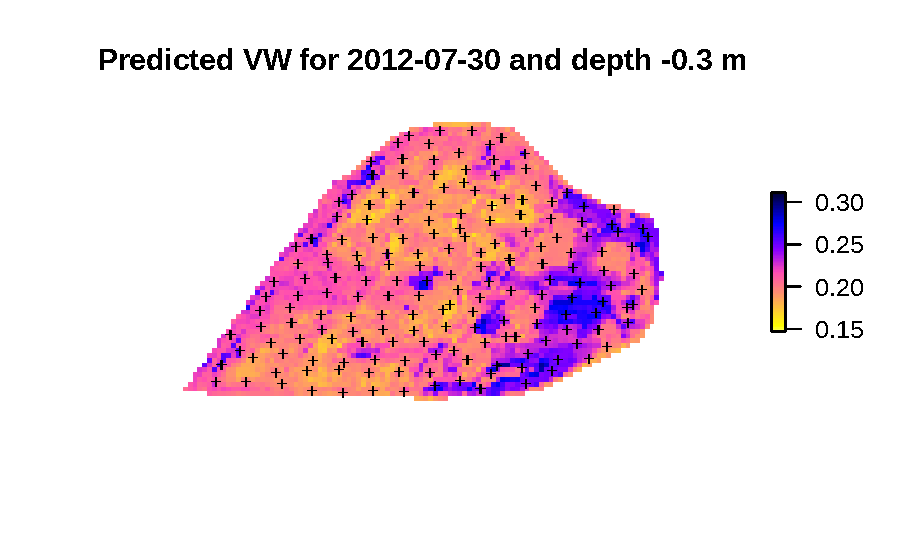
\includegraphics[width=0.9\linewidth]{resampling_st_files/figure-latex/map-eml-vw-1} 

}

\caption{Predicted soil water content based on spatiotemporal EML.}\label{fig:map-eml-vw}
\end{figure}

Because this is a spacetime dataset, we could also predict values of \texttt{VW} for
longer periods (e.g.~100 days) then visualize changes using e.g.~the \texttt{animation}
package or similar.

In summary this study also demonstrate the importance of resampling point data
using strict blocking of points that repeat in spacetime (measurement stations) is
important to prevent from overfitting. The difference between models fitted using
blocking per station and ignoring blocking can be drastic, hence how we
define and use resampling is important \citep{meyer2018improving}.

\hypertarget{generating-2nd-3rd-round-sampling}{%
\chapter{Generating 2nd, 3rd round sampling}\label{generating-2nd-3rd-round-sampling}}

You are reading the work-in-progress Spatial Sampling and Resampling for Machine Learning. This chapter is currently draft version, a peer-review publication is pending. You can find the polished first edition at \url{https://opengeohub.github.io/spatial-sampling-ml/}.

\hypertarget{uncertainty-guided-sampling}{%
\section{Uncertainty guided sampling}\label{uncertainty-guided-sampling}}

A sensible approach to improving quality of predictions is to: (a) estimate initial
ML models, (b) produce a realistic estimate of prediction errors, and (c) revisit
area and collect 2nd round samples that help at smallest possible costs significantly
improve predictions. Logical focus of the 2nd round sampling could be thus on minimizing
the overall prediction errors i.e.~revising parts of the study area that shows the
highest prediction errors / prediction problems (Fig. \ref{fig:eberg-var-eml}).
This is exactly procedure that \citet{stumpf2017uncertainty} recommend in their paper and
that they refer to as the \emph{``Uncertainty guided sampling''}.

The 2nd round Uncertainty guided sampling can be implemented either by:

\begin{itemize}
\tightlist
\item
  Producing a strata based on the prediction error map (e.g.~extrapolation areas / areas with highest uncertainty), then sampling only within that strata,
\item
  Using the probability of exceeding threshold mapping accuracy to generate extra sampling points,
\end{itemize}

In both cases 2nd round points can be then added to the original training dataset and the
model for the area can then be refitted (this procedure in data science is also referred to as \emph{``re-analysis''}).
Assuming that our initial model was unbiased, then even few tens of extra points
could lead to significant reduction in RMSPE. In practice, we might have to also
organize the 3rd round sampling until we finally reach some maximum possible accuracy \citep{hengl2018random}.

To generate 2nd round sampling for the Edgeroi dataset we can first estimate probability
of prediction errors exceeding some threshold probability e.g.~RMSE=0.2. We first
load point data and prediction error map produced in the previous example using
Ensemble Machine Learning:

\begin{Shaded}
\begin{Highlighting}[]
\FunctionTok{data}\NormalTok{(edgeroi)}
\NormalTok{edgeroi.sp }\OtherTok{\textless{}{-}}\NormalTok{ edgeroi}\SpecialCharTok{$}\NormalTok{sites}
\FunctionTok{coordinates}\NormalTok{(edgeroi.sp) }\OtherTok{\textless{}{-}} \ErrorTok{\textasciitilde{}}\NormalTok{ LONGDA94 }\SpecialCharTok{+}\NormalTok{ LATGDA94}
\FunctionTok{proj4string}\NormalTok{(edgeroi.sp) }\OtherTok{\textless{}{-}} \FunctionTok{CRS}\NormalTok{(}\StringTok{"+proj=longlat +ellps=GRS80 +towgs84=0,0,0,0,0,0,0 +no\_defs"}\NormalTok{)}
\NormalTok{edgeroi.sp }\OtherTok{\textless{}{-}} \FunctionTok{spTransform}\NormalTok{(edgeroi.sp, }\FunctionTok{CRS}\NormalTok{(}\StringTok{"+init=epsg:28355"}\NormalTok{))}
\end{Highlighting}
\end{Shaded}

The probability of exceeding some threshold, assuming normal distribution of prediction
erros can be derived as:

\begin{Shaded}
\begin{Highlighting}[]
\NormalTok{t.RMSE }\OtherTok{=} \FloatTok{0.2}
\NormalTok{edgeroi.error }\OtherTok{=} \FunctionTok{readGDAL}\NormalTok{(}\StringTok{"./output/edgeroi\_soc\_rmspe.tif"}\NormalTok{)}
\CommentTok{\#\textgreater{} ./output/edgeroi\_soc\_rmspe.tif has GDAL driver GTiff }
\CommentTok{\#\textgreater{} and has 321 rows and 476 columns}
\NormalTok{edgeroi.error}\SpecialCharTok{$}\NormalTok{inv.prob }\OtherTok{=} \DecValTok{1}\SpecialCharTok{/}\NormalTok{(}\DecValTok{1{-}2}\SpecialCharTok{*}\NormalTok{(}\FunctionTok{pnorm}\NormalTok{(edgeroi.error}\SpecialCharTok{$}\NormalTok{band1}\SpecialCharTok{/}\NormalTok{t.RMSE)}\SpecialCharTok{{-}}\FloatTok{0.5}\NormalTok{)) }
\end{Highlighting}
\end{Shaded}

next, we can generate a sampling plan using the \textbf{spatstat} package and the inverse
probability of the pixels exceeding threshold uncertainty (\texttt{f} argument):

\begin{Shaded}
\begin{Highlighting}[]
\NormalTok{dens.var }\OtherTok{\textless{}{-}}\NormalTok{ spatstat.geom}\SpecialCharTok{::}\FunctionTok{as.im}\NormalTok{(sp}\SpecialCharTok{::}\FunctionTok{as.image.SpatialGridDataFrame}\NormalTok{(edgeroi.error[}\StringTok{"inv.prob"}\NormalTok{]))}
\NormalTok{pnts.new }\OtherTok{\textless{}{-}}\NormalTok{ spatstat.core}\SpecialCharTok{::}\FunctionTok{rpoint}\NormalTok{(}\DecValTok{50}\NormalTok{, }\AttributeTok{f=}\NormalTok{dens.var)}
\end{Highlighting}
\end{Shaded}

So the new sampling plan, assuming adding only 50 new points would thus look like this:

\begin{Shaded}
\begin{Highlighting}[]
\FunctionTok{plot}\NormalTok{(}\FunctionTok{log1p}\NormalTok{(}\FunctionTok{raster}\NormalTok{(edgeroi.error[}\FunctionTok{c}\NormalTok{(}\StringTok{"inv.prob"}\NormalTok{)])))}
\FunctionTok{points}\NormalTok{(edgeroi.sp, }\AttributeTok{pch=}\StringTok{"+"}\NormalTok{, }\AttributeTok{cex=}\NormalTok{.}\DecValTok{8}\NormalTok{, }\AttributeTok{col=}\StringTok{"blue"}\NormalTok{)}
\FunctionTok{points}\NormalTok{(}\FunctionTok{as}\NormalTok{(pnts.new, }\StringTok{"SpatialPoints"}\NormalTok{), }\AttributeTok{pch=}\DecValTok{19}\NormalTok{, }\AttributeTok{cex=}\FloatTok{0.8}\NormalTok{, }\AttributeTok{col=}\StringTok{"black"}\NormalTok{)}
\end{Highlighting}
\end{Shaded}

\begin{figure}

{\centering 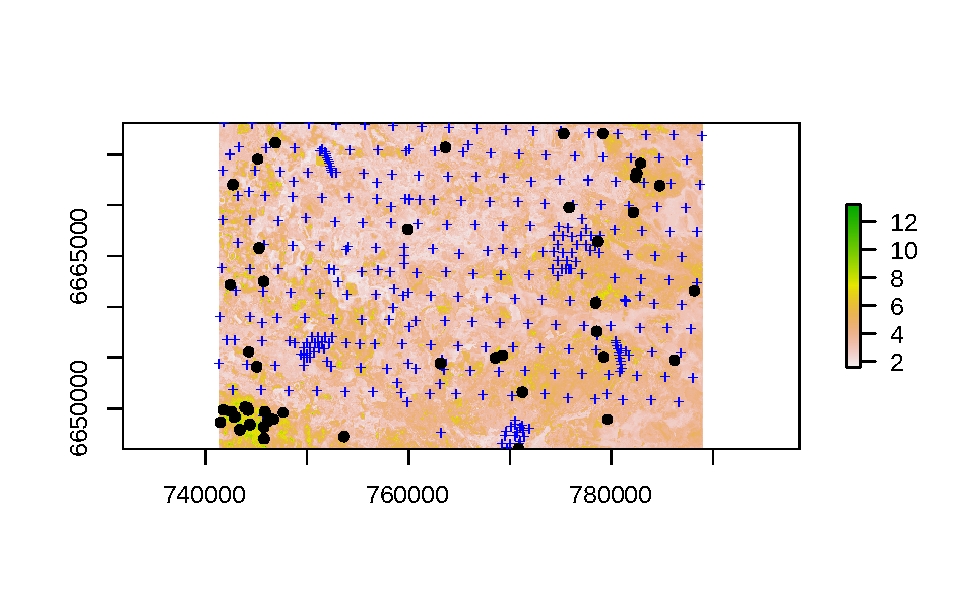
\includegraphics[width=1\linewidth]{extending_files/figure-latex/eberg-pnts-eml-1} 

}

\caption{Uncertainty guided 2nd round sampling: locations of initial (+) and 2nd round points (dots).}\label{fig:eberg-pnts-eml}
\end{figure}

This puts much higher weight at locations where the prediction errors are higher,
however, technically speaking we finish still sampling points across the whole
study area and, of course, including randomization.

\begin{figure}

{\centering \includegraphics[width=0.7\linewidth]{./img/Fig_sampling_reanalysis} 

}

\caption{General scheme for re-sampling and re-analysis using uncertainty guided sampling principles.}\label{fig:scheme-resample}
\end{figure}

By adding 2nd, 3rd round sampling we can imagine that the mapping accuracy / RMSE
would gradually decrease following a decay function (e.g.~\texttt{RMSE\ =\ b0\ *\ x\ \^{}\ -b1}) until some
maximum possible accuracy is achieved. This way soil surveyor can optimize the
predictions and reduce costs by minimizing number of additional samples i.e.~it
could be considered \emph{the shortest path} to increasing the mapping accuracy without
a need to start sampling from scratch.

\hypertarget{summary-notes}{%
\chapter{Summary notes}\label{summary-notes}}

You are reading the work-in-progress Spatial Sampling and Resampling for Machine Learning. This chapter is currently draft version, a peer-review publication is pending. You can find the polished first edition at \url{https://opengeohub.github.io/spatial-sampling-ml/}.

\hypertarget{which-sampling-algorithm-to-choose}{%
\section{Which sampling algorithm to choose?}\label{which-sampling-algorithm-to-choose}}

In this tutorial we have demonstrated some main steps required to analyze
existing sample designs (point patterns) and compare them with sampling algorithms
such as the SRC, LHS and FSCS. Some general conclusions are:

\begin{itemize}
\tightlist
\item
  Understanding limitations of spatial samples used for ML is important. Diversity of tools
  now exist that allow for sampling diagnostics, especially to determine spatial
  clustering, potential extrapolation areas, to test Complete Spatial Randomness etc;\\
\item
  Ensemble Machine Learning is at the order of magnitude more computational, but
  using combination of simple and complex base learners and spatial blocking seem to
  help produce models with less artifacts in extrapolation space and which report
  a more realistic mapping accuracy than if spatial clustering is ignored;\\
\item
  The \textbf{\href{https://rdrr.io/cran/forestError/}{forestError}} package seems to provide a complete framework for uncertainty
  assessment and can be used to derive the prediction errors (RMSPE) \emph{per-pixel}
  i.e.~for each new prediction location; the average prediction error
  of the whole area is the mean prediction error that one can report to the users
  as the best unbiased estimate of the mean uncertainty;
\end{itemize}

Figure below shows differences between the above mentioned sampling algorithms
in both geographical and feature spaces. In this case: actual sampling is
significantly missing the whole cluster in feature space, while FSCS seems to
show the highest spread in the feature space and by many authors is recognized
as the most advantageous sampling design for predictive mapping \citep{ma2020comparison}.
Such sampling diagnostics / comparisons geographical vs feature space help us
detect any possible problems before we start running ML.

\begin{figure}

{\centering 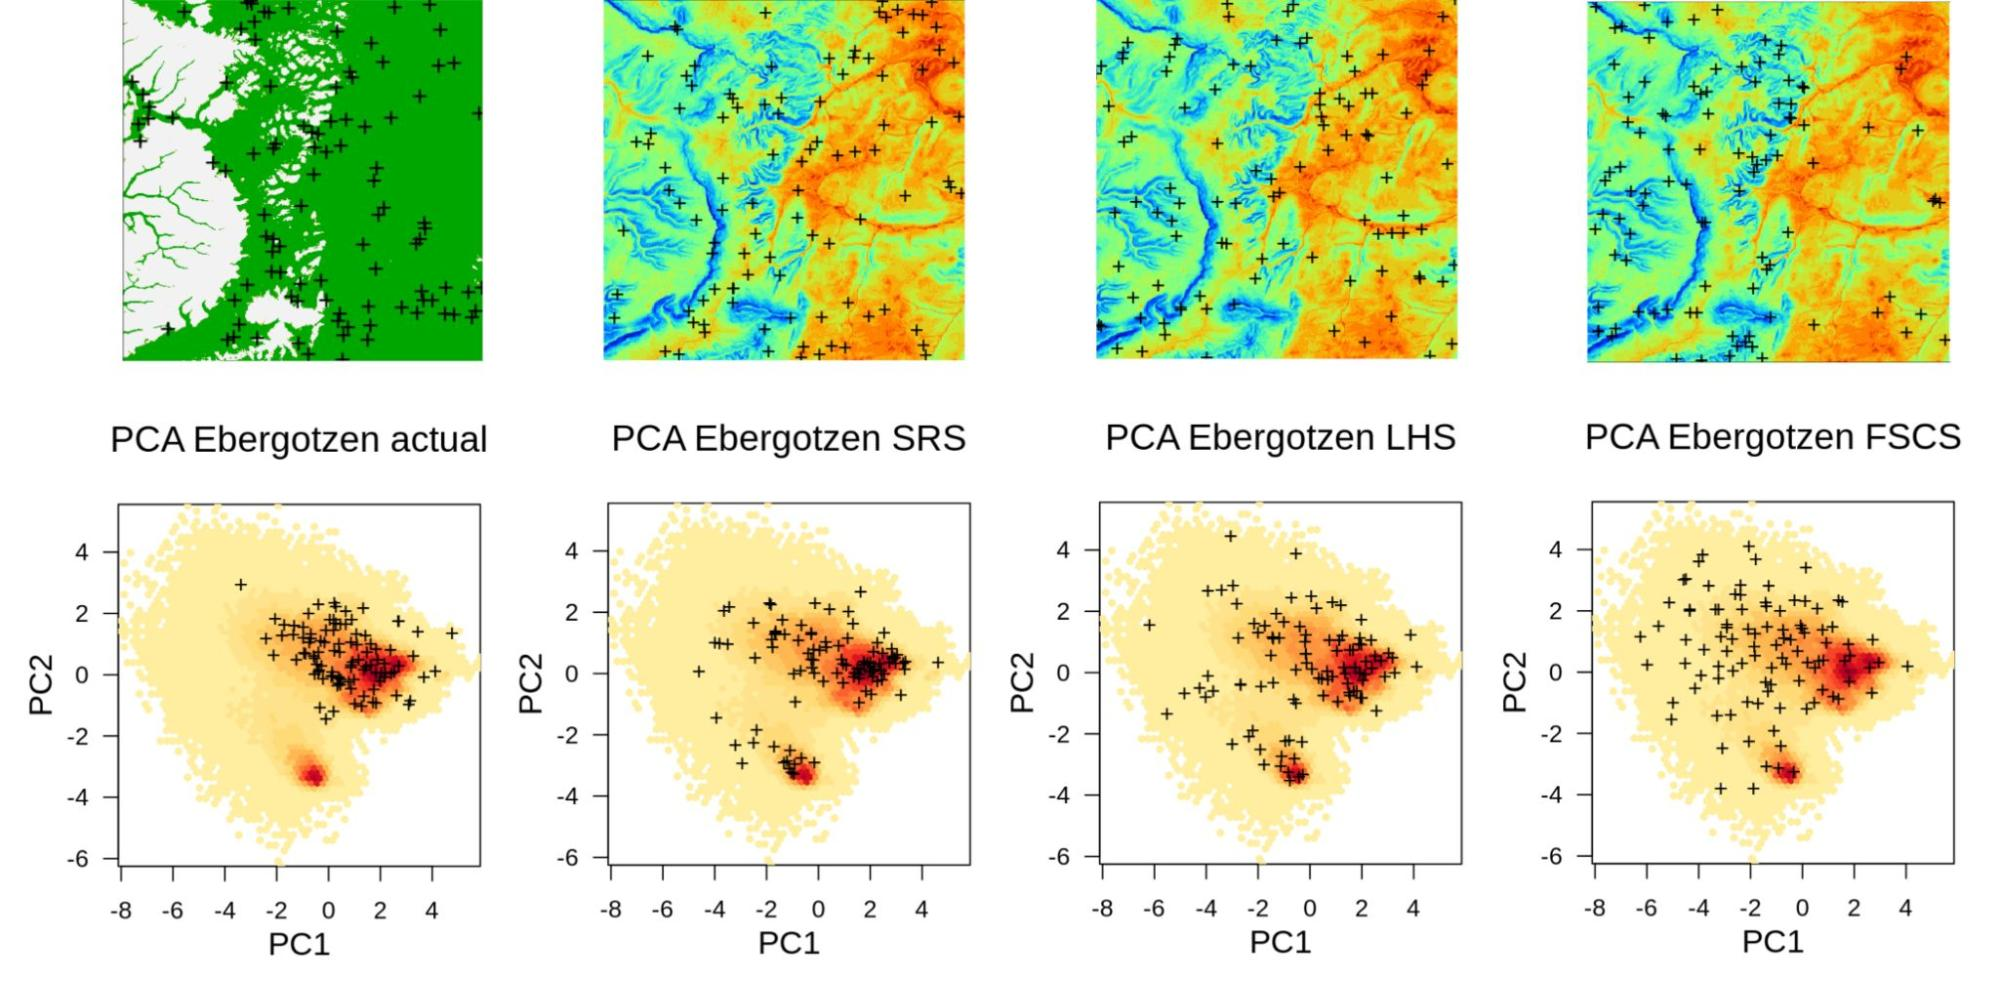
\includegraphics[width=1\linewidth]{./img/Fig_summary_comparison_sampling_eberg} 

}

\caption{Summary comparison of sampling designs: convenience sampling (actual), Simple Random Sample (SRS), Latin Hypercube Sampling (LHS), and Feature Space Coverage Sampling (FSCS). Points shown in geographical (above) and feature space (below; with first 2 principal components as x, y coordinates).}\label{fig:summary-eberg}
\end{figure}

\hypertarget{sampling-in-a-new-area}{%
\section{Sampling in a new area}\label{sampling-in-a-new-area}}

Recommended steps to prepare a sampling plan include:

\begin{enumerate}
\def\labelenumi{\arabic{enumi}.}
\tightlist
\item
  Prepare all covariate layers (rasters) that you plan to use to fit
  predictive mapping models; import them to R;
\item
  Convert covariate layers to Principal Components using the
  \textbf{\href{https://rdrr.io/cran/landmap/man/spc.html}{landmap::spc}}
  function;
\item
  Cluster the feature space using the
  \textbf{\href{https://docs.h2o.ai/h2o/latest-stable/h2o-docs/data-science/k-means.html}{h2o.kmeans}}
  function; for smaller number of samples use number of clusters equal
  to number of sampling locations;
\item
  Generate a sampling design and export the points to \textbf{\href{https://nl.wikipedia.org/wiki/GPS_Exchange_Format}{GPX
  format}} so they
  can be imported to a hand-held GPS or similar. For fieldwork we
  recommend using the \textbf{\href{https://play.google.com/store/apps/details?id=com.augmentra.viewranger.android\&hl=en\&gl=US}{ViewRanger
  app}}
  which has useful functionality for field work including planning the
  optimal routes.
\end{enumerate}

If you are collecting more than a few hundred points, then FSCS could
become cumbersome and we hence recommend using LHS sampling. This
sampling algorithm spreads points symmetrically in the feature space and
ensures that the extrapolation (in feature space) is minimized.

\hypertarget{ml-on-clustered-point-samples}{%
\section{ML on clustered point samples}\label{ml-on-clustered-point-samples}}

Assuming that there is significant spatial and/or feature space clustering in
training points, it appears that various blocking / Cross-Validation strategies,
especially based on Ensemble ML help produce more balanced estimate of regression
parameters and of the mapping accuracy. Incorporation of spatial proximity i.e.~
autocorrelation has roots in the \textbf{Generalized Least Squares methods} \citep{Venables2002Springer}
and in the classical data science papers e.g.~by \citet{roberts2017cross}. Ensemble ML
with spatial blocking comes, however, at the costs of the order of magnitude
higher computing costs.

In theory, even the most clustered point datasets can be used to fit predictive mapping models,
however, it is then important to use modeling methods that account for clustering and
prevent doing over-fitting and/or producing not realistic measures of mapping accuracy.
Eventually, very biased point samples totally missing ≫50\% of the feature / geographical
space would be of limited use for producing predictions, but could still be used to
get some initial estimates.

\citet{Wadoux2021EM} shows that, assuming that training points are based on the probability
sampling i.e.~SRS, there is no need for spatial blocking i.e.~regardless of the
spatial dependence structure in the target variable, any subset of SRS would give an
unbiased estimator of the mean population parameters. Many spatial statisticians
hence argue that mapping accuracy can be determined only by collecting data
using probability sampling \citep{Brus2011EJSS}. Indeed, we also recommend to users of these tutorials
to try your best to generate sampling designs using LHS, FSCS or at least SRS,
as this ensures unbiased derivation of population parameters. Here the book by
\citet{Brus2021sampling} seems to be a valuable resource as it also provides
\href{https://github.com/DickBrus/SpatialSamplingwithR}{practical instructions} for a diversity of data types.

If you have a dataset that you have used to test sampling and resampling, please
share your experiences by posting \href{https://github.com/OpenGeoHub/spatial-sampling-ml/}{an issue} and/or providing a screenshot of your results.

\hypertarget{references}{%
\chapter{References}\label{references}}

  \bibliography{./tex/refs.bib}

\backmatter
\printindex

\end{document}
